%CLASSE DOCUMENTO - LINGUA E DIMENSIONE FONT
\documentclass[11pt, a4paper, titlepage]{toptesi}

%%%%%%%%%%%%%%%%%%%%%%%%%%%%%%%%%%%%%%%%%%%%%%%%%%%%%%%%%%%%%%%

% INCLUSIONE PACCHETTI
\usepackage[utf8]{inputenc} %utf8
\usepackage[italian]{babel}
\usepackage[T1]{fontenc}
\usepackage{blindtext}
\usepackage{graphicx, wrapfig}
\usepackage{booktabs}
\usepackage{lmodern}
\usepackage{varioref}
\usepackage{url}
\usepackage{array}
\usepackage{paralist}{\obeyspaces\global\let =\space}
\usepackage{verbatim}
\usepackage{subfig}
\usepackage{amsmath}
\usepackage{amsfonts}
\usepackage{amssymb}
\usepackage{multicol}
\usepackage{multirow}
\usepackage{listings}
\usepackage[pass]{geometry}
\usepackage[figuresright]{rotating}
\usepackage{algorithm}
\usepackage{algorithmic}
\usepackage{amsmath}
\usepackage[babel]{csquotes}
\usepackage{hyperref}
\usepackage[backend=bibtex]{biblatex}
\usepackage{xcolor}
\usepackage{enumitem}
\usepackage{titlesec}
\usepackage{booktabs}   % this package promotes good tabular style
\usepackage{caption}    % for customising caption style
\usepackage{siunitx}    % for decimal alignment
\usepackage{dirtytalk}
\usepackage{lipsum,caption,graphicx}
%\usepackage{theorems}
%\usepackage{tabularx}
\usepackage{amsthm} % Mi dava problemi il package theorems, ho risolto con questo.
\usepackage[swapnames]{frontespizio}

%%%%%%%%%%%%%%%%%%%%%%%%%%%%%%%%%%%%%%%%%%%%%%%%%%%%%%%%%%%%%%%

\theoremstyle{definition}
\newtheorem{example}{Esempio}[section]

\definecolor{cosmogreen}{RGB}{61, 176, 23}
\definecolor{cosmoorange}{RGB}{255, 117, 24}
\definecolor{cosmoblue}{RGB}{25, 103, 190}
\definecolor{cosmored}{RGB}{255, 0, 57}
\definecolor{cosmoblack}{RGB}{55, 58, 60}

% CONFIGURAZIONE LINK E RIFERIMENTI
\hypersetup{%
    pdfpagemode={UseOutlines},
    bookmarksopen,
    pdfstartview={FitH},
    colorlinks,
    linkcolor={cosmoblack}, %COLORE DEI RIFERIMENTI AL TESTO
    citecolor={cosmoblue}, %COLORE DEI RIFERIMENTI ALLE CITAZIONI
    urlcolor={cosmoblue} %COLORI DEGLI URL
}

%%%%%%%%%%%%%%%%%%%%%%%%%%%%%%%%%%%%%%%%%%%%%%%%%%%%%%%%%%%%%%%

% CONFIGURAZIONE LISTATI/CODICE


\lstset{frame=tb,
  keywords = {EXPECT_EQ, TEST, std::string, Bytes}
  language=C++,
  aboveskip=3mm,
  belowskip=3mm,
  showstringspaces=false,
  columns=flexible,
  basicstyle={\small\ttfamily},
  numbers=left,
  numberstyle=\tiny\color{cosmoblack},
  keywordstyle=\color{cosmoblue},
  commentstyle=\color{cosmoorange},
  stringstyle=\color{cosmogreen},
  breaklines=true,
  breakatwhitespace=true,
  tabsize=3
}


\lstset{frame=tb,
  keywords = {__init__}
  language=Python,
  aboveskip=3mm,
  belowskip=3mm,
  showstringspaces=false,
  columns=flexible,
  basicstyle={\small\ttfamily},
  numbers=left,
  numberstyle=\tiny\color{cosmoblack},
  keywordstyle=\color{cosmoblue},
  commentstyle=\color{cosmoorange},
  stringstyle=\color{cosmogreen},
  breaklines=true,
  breakatwhitespace=true,
  tabsize=3
}

% definizione BITCOIN script
\lstdefinelanguage{bitcoinscript}{
    alsodigit = {-},
    keywords = {OP_DUP,OP_HASH160,OP_EQUALVERIFY,OP_CHECKSIG, OP_CHECKMULTISIG,
                OP_0, OP_2, OP_3, OP_EQUAL, OP_RETURN, OP_IF, OP_CHECKLOCKTIMEVERIFY,
                OP_DROP, OP_CHECKSIGVERIFY, OP_ELSE, OP_ENDIF, OP_CHECKMULTISIG, OP_ELSE,
                OP_ENDIF, OP_SWAP, OP_ADD, OP_VERIFY, OP_PUSHDATA1},
    aboveskip=3mm,
    belowskip=3mm,
    showstringspaces=false,
    columns=flexible,
    basicstyle={\small\ttfamily},
    numbers=left,
    numberstyle=\tiny\color{cosmoblack},
    keywordstyle=\color{cosmoblue},
    commentstyle=\color{cosmoorange},
    stringstyle=\color{cosmogreen},
    breaklines=true,
    breakatwhitespace=true,
    tabsize=3
}

%Definizione MINISCRIPT
\lstdefinelanguage{miniscript}{
    keywords = {thresh,pk,older},
    aboveskip=3mm,
    belowskip=3mm,
    showstringspaces=false,
    columns=flexible,
    basicstyle={\small\ttfamily},
    numbers=left,
    numberstyle=\tiny\color{cosmoblack},
    keywordstyle=\color{cosmoblue},
    commentstyle=\color{cosmoorange},
    stringstyle=\color{cosmogreen},
    breaklines=true,
    breakatwhitespace=true,
    tabsize=3
}

\lstdefinelanguage{JSON}{
    aboveskip=3mm,
    belowskip=3mm,
    showstringspaces=false,
    columns=flexible,
    basicstyle={\small\ttfamily},
    numbers=left,
    numberstyle=\tiny\color{cosmoblack},
    keywordstyle=\color{cosmoblue},
    commentstyle=\color{cosmoorange},
    stringstyle=\color{cosmogreen},
    breaklines=true,
    breakatwhitespace=true,
    tabsize=3
}

\setitemize{noitemsep,topsep=0pt,parsep=0pt,partopsep=0pt}
\setenumerate{noitemsep,topsep=0pt,parsep=0pt,partopsep=0pt}
\setdescription{noitemsep,topsep=0pt,parsep=0pt,partopsep=0pt}
\setlist{noitemsep,topsep=0pt,parsep=0pt,partopsep=0pt}

%Spazio tra le sezioni con un pacchetto aggiuntivo
\titlespacing\section{0pt}{12pt plus 4pt minus 2pt}{0pt plus 2pt minus 2pt}
\titlespacing\subsection{0pt}{12pt plus 4pt minus 2pt}{0pt plus 2pt minus 2pt}
\titlespacing\subsubsection{0pt}{12pt plus 4pt minus 2pt}{0pt plus 2pt minus 2pt}

%Impostazion centraggio Tabella
\newcolumntype{C}[1]{>{\centering\arraybackslash}p{#1}}

%%%%%%%%%%%%%%%%%%%%%%%%%%%%%%%%%%%%%%%%%%%%%%%%%%%%%%%%%%%%%%%

% FRENCHSPACING VA _SEMPRE_ ABILITATO PER DOCUMENTI IN ITALIANO
\frenchspacing

%%%%%%%%%%%%%%%%%%%%%%%%%%%%%%%%%%%%%%%%%%%%%%%%%%%%%%%%%%%%%%%

%DEFINIZIONE SEZIONI IN NUMERAZIONE ROMANA
%ELENCO DEI LISTATI/CODICI
\makeatletter
\newcommand\listofcodes{%
 \iffrontmatter\else\frontmattertrue\fi
 \if@openright\cleardoublepage\else\clearpage\fi
 % change the meaning of \chapter in a group
 \begingroup\def\chapter##1{\@schapter}
 \phantomsection % for the hyperlink
 \lstlistoflistings
 \endgroup
}
\newcommand{\source}[1]{\caption*{Fonte: {#1}} }
\makeatother

\renewcommand*\lstlistingname{Codice}
\renewcommand*\lstlistlistingname{Lista dei codici}

%%%%%%%%%%%%%%%%%%%%%%%%%%%%%%%%%%%%%%%%%%%%%%%%%%%%%%%%%%%%%%%

%%%%%%%%%%%%%%%%%%%%%%%%%%%%%%%%%%%%%%%%%%%%%%%%%%%%%%%%%%%%%%%

% LISTA DEI CAPITOLI DA INCLUDERE - PERSONALIZZARE
\includeonly{%
chap_blockchain,%
chap_bitcoin,%
chap_bitcoincore,%
chap_problema,%
chap_riferimenti_storici,%
chap_tecnologie_utilizzate,%
chap_soluzione_proposta,%
chap_conclusioni,%
app_a,%
}

% FILE DI BIBLIOGRAFIA
\bibliography{bibliography}


%%%%%%%%%%%%%%%%%%%%%%%%%%%%%%%%%%%%%%%%%%%%%%%%%%%%%%%%%%%%%%%

% INIZIO DOCUMENTO
\begin{document}

\begin{frontespizio}
\Margini{2.5cm}{3cm}{2.5cm}{3.5cm}
\Preambolo{\renewcommand{\fronttitlefont}{\fontsize{24}{32}\bfseries}}% questo era proprio sbagliato (agisci su 32 se vuoi modificare lo spazio interlinea
\Preambolo{\renewcommand{\frontpretitlefont}{\fontsize{14}{14}\scshape}}
\Preambolo{\renewcommand{\frontinstitutionfont}{\fontsize{17}{17}\scshape}}
\Preambolo{\renewcommand{\frontdivisionfont}{\fontsize{12}{40}\normalfont}}% modifica il 40 finché trovi quello che desideri
\Preambolo{\renewcommand{\frontfixednamesfont}{\fontsize{12}{12}\normalfont}}
\Preambolo{\renewcommand{\frontnamesfont}{\fontsize{12}{12}\bfseries\vspace{5cm}}}
\Logo[3cm]{images/unibas-logo.png}
\Istituzione {Università degli studi della Basilicata}
\Divisione {Scuola di Ingegneria}
\vspace{2mm}
\Corso [Laurea Triennale]{Scienze e tecnologie informatiche}
\Titoletto {Tesi in Basi di dati}
\Titolo {Estrazione d'informazioni dalla \\blockchain di Bitcoin​}
\Candidato {Palazzo Vincenzo}
\Relatore {Dott.\\Carlo Sartiani}
\Annoaccademico {2018-2019}
\end{frontespizio}

%%%%%%%%%%%%%%%%%%%%%%%%%%%%%%%%%%%%%%%%%%%%%%%%%%%%%%%%%%%%%%%

%INTERLINEA - DEFAULT 1 - NON ESAGERATE, NON SUPERATE MAI 1.3 ;)
%\interlinea{1.3}

%%%%%%%%%%%%%%%%%%%%%%%%%%%%%%%%%%%%%%%%%%%%%%%%%%%%%%%%%%%%%%%

\frontmatter

% CITAZIONE - PERSONALIZZARE
% VSPACE - PROPORZIONE USATA PER CENTRATURA VERTICALE DEL TESTO
% FLUSHRIGHT - ALLINEAMENTO ORIZZONTALE A DESTRA
\vspace*{\stretch{1}}
\begin{flushright}
\noindent
Non è tanto chi sono ma quello\\ che faccio che mi qualifica.

\textit{Bruce Wayne}
\end{flushright}
\vspace*{\stretch{6}}
\cleardoublepage

%%%%%%%%%%%%%%%%%%%%%%%%%%%%%%%%%%%%%%%%%%%%%%%%%%%%%%%%%%%%%%%

% ABSTRACT - PERSONALIZZARE
\sommario
Piacere, sommario.

%%%%%%%%%%%%%%%%%%%%%%%%%%%%%%%%%%%%%%%%%%%%%%%%%%%%%%%%%%%%%%%

% INDICE GENERALE
\tableofcontents

\mainmatter

% INCLUSIONE FILE CAPITOLI - PERSONALIZZARE - TENERE COERENTE CON LISTA IN ALTO
\chapter{Blockchain}
\label{chap:blockchain}

\section{Introduzione}
\label{sec:introduzione}

Il termine \emph{blockchain} denota un particolare tipo di \emph{distributed ledger} protetto mediante meccanismi crittografici.
Il distributed ledger è un log distribuito, parzialmente o totalmente replicato a cui accedono un gruppo di peer.
All’interno di una blockchain vengono memorizzate in modo permanente e immutabile una serie di informazioni verificate attraverso opportuni algoritmi di consenso.\\
La prima tecnologia ad introdurre il concetto di blockchain fu Bitcoin\footnote{Utilizzeremo per tutto il documento la convenzione sulla parola Bitcoin, scritta con la lettera maiuscola indicherà il protocollo Bitcoin, analogamente per bitcoin scritto con la lettera minuscola che indicherà la moneta.}, la quale utilizza una struttura dati per la memorizzazione che fa uso del concetto di \say{blocco}; i blocchi sono concatenati attraverso una \emph{hash pointer} e contengono un quantitativo variabile di transazioni.\\
Le transazioni sono l'unico modo per scatenare eventi che mutano lo stato della blockchain e la struttura di esse varia in base al tipo di informazioni da memorizzare; in seguito alla tecnologia Bitcoin vengono presentate altre blockchain che apportano una serie di modifiche alla struttura dati utilizzata.


\section{Protocolli di consenso}
\label{sec:protocolloDiConsenso}

Gli algoritmi di consenso assicurano che il nuovo blocco da pubblicare sulla blockchain sia completamente convalidato e protetto, assicurando anche che le transazioni siano valide; questi algoritmi svolgono un ruolo fondamentale nella risoluzione del problema della doppia spesa.
Il protocollo introdotto dalla prima tecnologia blockchain, cioè Bitcoin, è l’algoritmo di  Proof of Work (PoW) dove, per dimostrare la validità di un blocco e il lavoro svolto, i nodi nella rete (chiamati {\it miner\/}) usano potenza computazionale per convalidare le azioni e competono tra loro in una sfida crittografica per trovare una soluzione ad un problema imposto dal protocollo.
Il vincitore ha diritto ad una ricompensa per la vincita e, se il protocollo lo prevede, a riscuotere le commissioni incluse nelle transazioni.
Il miner vincitore della sfida creerà un nuovo blocco, includendo l’hash del blocco precedente, il timestamp e le transazioni. \\
Trasmettendo il nuovo blocco sulla rete, si può verificare un fenomeno di concorrenza: due o più nodi possono pubblicare un blocco con lo stesso hash di blocco precedente, ma contenuto completamente o parzialmente differente. Tale fenomeno viene aggirato scegliendo di lavorare con una catena di blocchi più lunga, perché in quel caso il miner avrà svolto maggior lavoro. \\
Come ogni protocollo, i protocolli di consenso presentano vulnerabilità: in teoria, il protocollo PoW può essere attaccato se un miner, da solo o in un gruppo, possiede più della metà della potenza di estrazione totale della rete. Questo è anche noto come \emph{attacco del 51\%} in cui gli aggressori creano la propria catena segreta riuscendo ad ottenere la fiducia di tutto il sistema, compromettendone quindi le funzionalità.


\section{Blocchi}
\label{sec:blocchiBlockchain}

La blockchain può essere definita come una struttura ad albero con zero o al massimo un figlio; ogni blocco contiene il riferimento al blocco precedente, con cui si ottiene una relazione padre-figlio a tutti gli effetti.
Concatenando tutti i blocchi con i relativi padri, si ottiene un unico percorso con cui attraversare la blockchain, che può anche essere vista come una lista di blocchi concatenati singolarmente.
Il link che funge da collegamento tra i due blocchi è un puntatore crittografico chiamato comunemente {\it hash pointer\/}, generato da una funzione hash, applicata alla concatenazione delle informazioni del blocco in un preciso ordine. La Tabella \ref{tab:bitcoinblock} riporta una rappresentazione generale del blocco.


\begin{table}[ht]
       \centering\small
           \begin{tabular}{|c|}
               \hline
               \textbf{Block}\\
               \hline \hline
               Prova di lavoro (nonce)   \\
               \hline
               Transazioni valide \\
               \hline
               Timestamp \\
               \hline
               Merkle Tree \\
               \hline
       \end{tabular}
       \caption{Rappresentazione generale del concetto di blocco in una blockchain.\label{tab:bitcoinblock}}
   \end{table}



\begin{itemize}
  \item {\bf Nonce\/}: Esso funge da contenitore del valore usato nella PoW e il suo valore è un numero casuale che rappresenta il valore di difficoltà con cui è stato costruito il blocco.
  \item {\bf Timestamp\/}: Valore che indica la data di pubblicazione del blocco.
\end{itemize}
\leavevmode
\\
I Merkle tree furono inventati da Ralph Merkle nel 1988, nel tentativo di costruire migliori firme digitali; questa struttura in una blockchain ha lo scopo di diminuire il costo sulla verifica delle transazioni, senza dover accedere singolarmente ad esse, e di conseguenza fornisce un modo per verificare la correttezza dell’intera blockchain.
La costruzione di questo albero inizia dalle foglie, dove ogni foglia contiene il valore hash calcolato tramite una funzione unidirezionale come MD5 oppure SHA-1, procedendo così alla creazione dei nodi interni che corrispondono alla funzione hash della concatenazione dei figli.
Utilizzando la funzione hash nella costruzione della struttura ad albero, viene garantita l’integrità delle informazioni: ciò vuol dire che, se qualche malintenzionato cambiasse il valore all’interno di una foglia, tutto il cammino radice foglia sarebbe alterato, con un cambiamento inevitabile anche della radice.
La proprietà di questa funzione vieta a chiunque di alterare le informazioni relative alle transazioni all’interno di un blocco una volta reso pubblico; ciò rende impossibile, ad esempio, aggiungere una transazione, rimuoverla o modificarla, come mostrato in Figura \ref{fig:merkletree}.

\begin{figure}[H]
\begin{center}
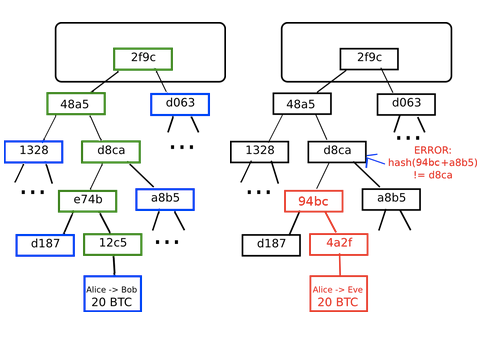
\includegraphics[width=0.6\columnwidth]{images/image-merkle-treepng.png}
\end{center}
\caption{Esempio di stato non valido per un cammino radice foglia. \cite{ethereum:paper}}
\label{fig:merkletree}
\end{figure}

\chapter{Bitcoin}
\label{chap:bitcoin}

\section{Introduzione}
\label{sec:introduzione}

Bitcoin introdusse per primo il concetto di blockchain: ciò permise la creazione di un metodo di pagamento peer-to-peer esente da un intermediario, definito anche come criptovaluta decentralizzata.
Introdotto da una persona o un gruppo di persone sotto lo pseudonimo di \say{Satoshi Nakamoto}, Bitcoin viene descritto per la prima volta nel white paper intitolato \say{Bitcoin: A Peer-to-Peer Electronic Cash System} pubblicato nell’ottobre 2008 sulla mailing list di crittografia del sito \url{https://www.metzdowd.com}.\newline
Il 3 gennaio 2009 venne rilasciata la versione 0.1 del codice sorgente sotto licenza MIT da Satoshi Nakamoto che smise di contribuire al progetto nel dicembre 2011. Si stima che ad oggi Satoshi Nakamoto possegga un milione di bitcoin\footnote{Un milione di bitcoin equivale a 9297736092.00 di euro, nel 16/07/2019}, sparsi in vari wallet.

\section{Transazioni}
\label{sec:transazioniBitcoin}

Le transazioni sono una parte fondamentale di Bitcoin. Infatti tutto il sistema è progettato per assicurare la creazione, propagazione e pubblicazione di transazioni su blockchain, ma queste ultime sono concettualmente differenti dalle transazioni a cui siamo abituati: ad esempio, una transazione di un database relazionale rappresenta un evento che innesca un cambio di stato all’interno della base di dati, dove in caso di malfunzionamenti la base di dati ritorna nella condizione precedente, prima che l’evento fosse scatenato.
Le transazioni di Bitcoin sono concettualmente differenti.


\begin{example}
\label{example:aliceBobFirst}
Consideriamo il seguente scenario con i seguenti personaggi:

\begin{itemize}
  \item Alice e Bob sono due utenti che usano attivamente Bitcoin per effettuare i loro pagamenti.
  \item Vincent è un partecipante della rete di Bitcoin e si occupa di effettuare il mining (argomento trattato nella Sezione \ref{sec:miningbitcoin}) per proteggere la rete e trarre ricavi in bitcoin.
\end{itemize}

Alice ha deciso di inviare 0.00700767 bitcoin a Bob; Alice dopo aver ottenuto l’indirizzo Bitcoin di Bob, che corrisponde a \say{33mMAc6nGyENdKMQTr5SrKoEkwNTeZQUx9}, può inviare dei bitcoin a Bob, generando una nuova transazione con il seguente identificativo: \say{ddd587d54b693a9bc9bda2218c6f5e17979f6ac53755c5c1f668f3fa728e472d}.\newline
Questa nuova transazione consuma una precedente transazione in possesso di Alice, chiamata UTXO (\emph{unspent transaction output}), e crea un nuovo UTXO in possesso di Bob; la nuova transazione viene verificata da un componente (nodo) della rete, in questo caso Vincent.

{\centering
\vspace{15pt}
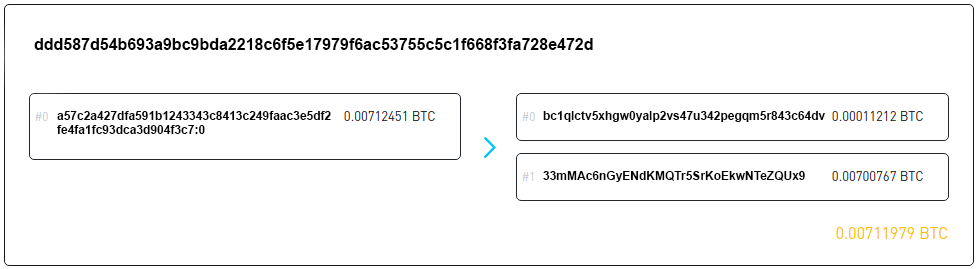
\includegraphics[scale=0.35]{images/example_alice_bob_vincent.png}
\captionof{figure}{La nuova transazione creata da Alice ricercata attraverso un explorer \cite{blockstream:esplora}.\label{fig:examplealicebob}}
\vspace{10pt}
\par}

Come illustrato in Figura \ref{fig:examplealicebob}, l'operazione di Alice provoca lo spostamento di bitcoin da una precedente transazione con il seguente identificativo: \say{a57c2a427d\-fa591b1243\-343c8413c249\-faac3e5df2fe4fa1fc93dca3d904f3c7} a due diversi indirizzi, cioè:

\begin{itemize}

  \item 33mMAc6nGyENdKMQTr5SrKoEkwNTeZQUx9 (indirizzo Bitcoin di Bob);

  \item bc1qlctv5xhgw0yalp2vs47u342pegqm5r843c64dv (indirizzo Bitcoin di Alice): poiché gli UTXO sono indivisibili, essi devono venire consumati interamente.  Nel momento in cui si genera una nuova transazione viene scelto l’UTXO più adatto con un valore di bitcoin uguale al valore da inviare a Bob; se questo non esiste, si seleziona l'UTXO \emph{best fit},  con la conseguenza che il wallet genererà una nuova transazione (conosciuta come \emph{exchange transaction}) verso se stesso per recuperare i bitcoin rimanenti. Questo processo è illustrato in Figura \ref{fig:examplechangeutxo}.


%  la motivazione della generazione di un UTXO verso Alice, che in questo esempio ha generato una nuova transazione per inviare bitcoin a Bob, è il seguente:  gli UTXO di Alice non vengono mischiati e messi insieme ma bensì gli UTXO sono unità indivisibili e vengono mantenuti separatamente come illustrato in Figura \ref{fig:examplechangeutxo}.

  \begin{figure}[h]
  \begin{center}
  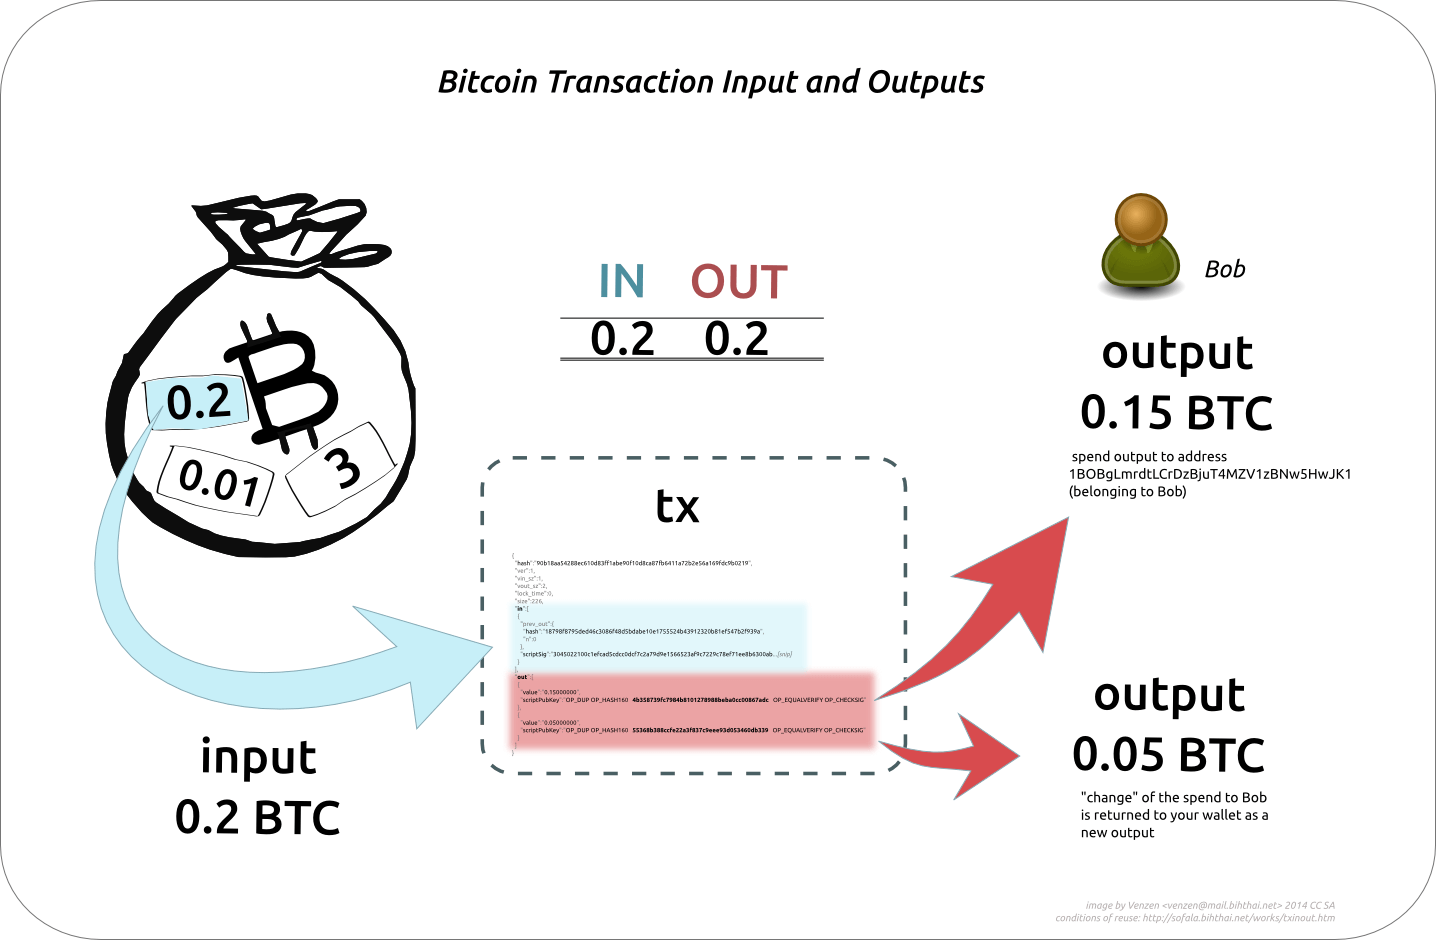
\includegraphics[width=0.6\columnwidth]{images/change_utxo.png}
  \end{center}
  \caption{Gestione degli UTXO nella blockchain di Bitcoin \cite{blockstream:esplora}.}
  \label{fig:examplechangeutxo}
  \end{figure}
%  Nel momento in cui si genera una nuova transazione viene scelto l’UTXO può adatto con un valore di bitcoin uguale al valore da inviare nella nuova transazione se questo non esiste si seleziona l’UTXO con un valore maggiore di bitcoin con la conseguenza che il wallet genererà una nuova transazione verso se stesso per recuperare i bitcoin rimanenti; come quanto si effettua un pagamento di 25 euro in un ristorante con una banconota da 50 euro in cui bisogna restituire 25 euro di resto.
%  \item 33mMAc6nGyENdKMQTr5SrKoEkwNTeZQUx9: Indirizzo Bitcoin di Bob.
\end{itemize}

La verifica della nuova transazione di Alice viene effettuata da Vincent, il quale inserisce la transazione in un nuovo blocco insieme a tutte le altre pubblicate sulla rete in quel momento.

Nel momento in cui viene pubblicato il blocco il sistema crea una transazione verso Vincent come premio per il lavoro svolto; questa nuova transazione è conosciuta con il nome di transazione \emph{coinbase} ed è mostrata in Figura \ref{fig:examplecoinbasetxvincent}.

{\centering
\vspace{15pt}
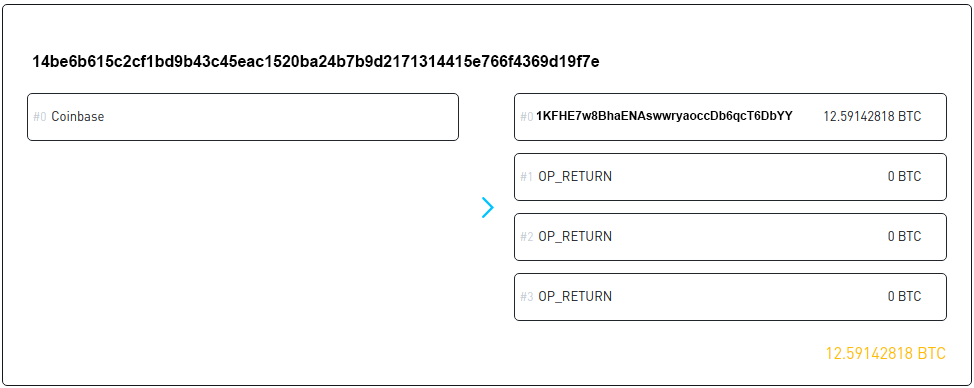
\includegraphics[scale=0.35]{images/example_coinbase_vincent.png}
\captionof{figure}{Transazione coinbase descritta  \cite{blockstream:esplora}.\label{fig:examplecoinbasetxvincent}}
\vspace{10pt}
\par}

\end{example}

L'esempio precedente mostra come  in Bicoin si possano distinguere due tipi: la transazione {\it coinbase\/} e la transazione comune.
\begin{itemize}
  \item La transazione coinbase è un evento speciale che si verifica sul sistema, il cui formato risulta non valido per la blockchain, poiché la sua struttura contiene zero input e un output. Questo evento rappresenta nel sistema un’emissione di nuovi bitcoin (argomento trattato nella Sezione \ref{sec:miningbitcoin}), rendendo la transazione coinbase una transazione speciale per il sistema Bitcoin.
  \item Una transazione comune è un evento che punta a sbloccare una transazione esistente su blockchain, conosciuta come UTXO, allo scopo di   creare un movimento di bitcoin.
\end{itemize}

Possono verificarsi principalmente due tipi di fallimenti durante la creazione di una transazione:
\begin{enumerate}
  \item Una transazione non è valida per il sistema Bitcoin; in questo caso esso viene inoltrata alla rete come una transazione valida, ma essa verrà rigettata dal primo nodo completo\footnote{Per nodo completo viene inteso un nodo che possiede l’intera copia della blockchain ed è abilitato per la validazione di transazioni; esso viene utilizzato comunemente dai miner.} utile. Un esempio di transazione non valida è una transazione che contiene zero input ed un output.
  \item Una transazione valida per il sistema ma non valida per sbloccare UTXO: essa viene accettata dal sistema Bitcoin perché valida, ma la transazione non è capace di sbloccare nessun UTXO. Un esempio è costituito da  una transazione che prova a spendere due volte lo stesso UTXO (evento di doppia spesa).
\end{enumerate}
Bitcoin pertanto descrive le transazioni come \say{consumabili}, cioè una transazione di input consuma un UTXO e nello stesso istante produce un UTXO ex novo.
\begin{example}
Consideriamo nuovament l'esempio precedente  e supponiamo che Bob abbia deciso di inviare parte dei bitcoin ricevuti da Alice a Sara. Una volta ottenuto l’indirizzo Bitcoin di Sara, cioè \say{3CM8TuY8B3\-sCzVQN3FWYnd5skmzSF3uvWA}, per effettuare il trasferimento Bob  crea una nuova transazione di 0.00137927 bitcoin con il seguente identificativo \say{907538047d630d571298096028572\-08705ef3baa4b573e6e845d5a3e6ea\-11464}, raffigurata in Figura \ref{fig:examplebobsara}.
%Credo che sia colpa di questa immagine per lo spazio precedente.
{\centering
\vspace{15pt}
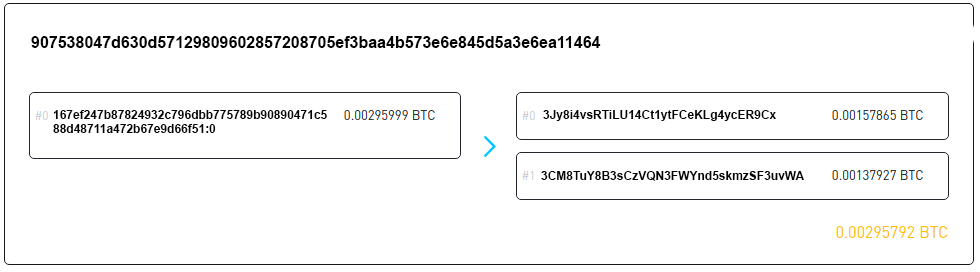
\includegraphics[scale=0.35]{images/example_bob_sara.png}
\captionof{figure}{La transazione creata da Bob verso Sara \cite{blockstream:esplora}.\label{fig:examplebobsara}}
\vspace{10pt}
\par}

%In questo scenario viene illlustrato il modo in cui Bob utilizza il suo UTXO per creare una nuova transazione verso Sara; come illustrato nella Figura \ref{fig:examplechangeutxo} gli UTXO non sono raggruppati ma quest’ultimi vengono contenuti all’interno di un'aria in cui risiedono tutti gli UTXO: quindi in questo esempio Bob deve fornire una prova che la transazione sia effettivamente sua, inoltre in seguito deve utilizzare un modo per cui Sara (solo lei) sarà in grado di spendere il suo UTXO.

Poiché gli UTXO sono contenuti all’interno di un'area in cui risiedono tutti gli UTXO, Bob deve fornire una prova che la transazione UTXO che vuole consumare sia effettivamente sua; inoltre in seguito deve utilizzare un modo per cui solo Sara  sarà in grado di spendere il suo UTXO.

A tale scopo Bitcoin offre un sistema di blocco delle transazioni di output e un sistema di sblocco per le transazioni di input.  Questo sistema si basa sull'impiego di script (argomento trattato nella Sezione \ref{sec:bitcoinScriptBitcoin}) che utilizzano estensivamente tecniche crittografiche con cui è possibile verificare la proprietà di quell'UTXO.
Nell'esempio in cui Alice crea una nuova transazione per Bob, per rendere la transazione sbloccabile solo da Bob, Alice ha inserito all’interno dello script di blocco dell’UTXO la chiave pubblica di Bob.\newline
Bob per creare una transazione verso Sara deve sbloccare l’UTXO che gli appartiene fornendo all’interno dello script di sblocco (contenuto all’interno la transazione di input) la firma della sua chiave privata e in un secondo momento deve creare un UTXO sbloccabile solo da Sara inserendo all’interno lo script di blocco la chiave pubblica di Sara.\newline
In Figura \ref{fig:lockunlockexample} viene rappresentato il flusso di eventi che descrive il blocco e sblocco di un UTXO.

{\centering
\vspace{5pt}
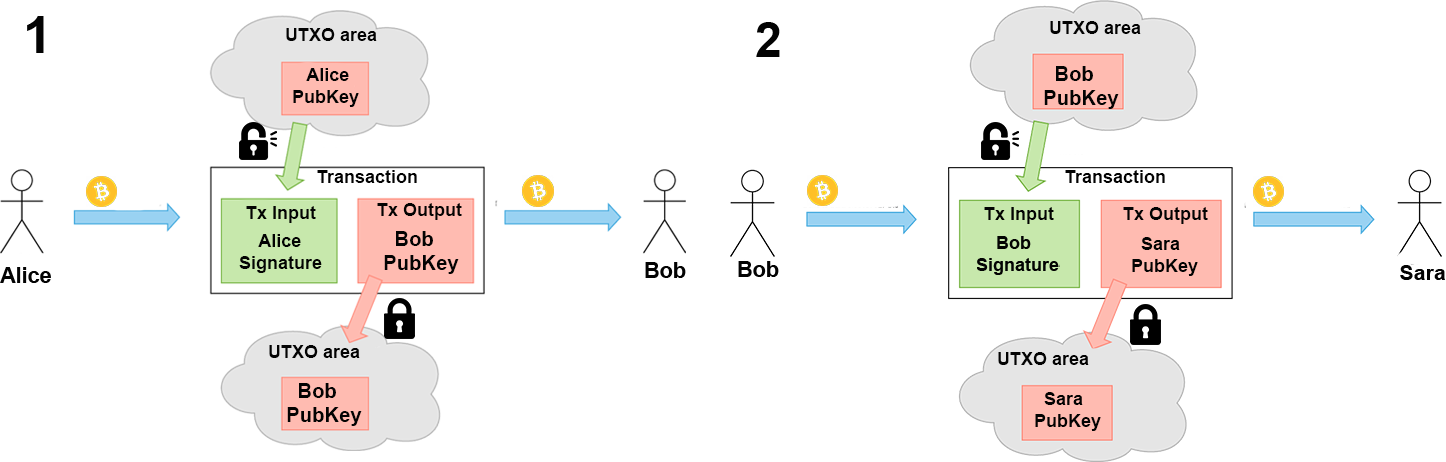
\includegraphics[scale=0.2]{images/DiagramUnlocLockUTXO.png}
\captionof{figure}{Rappresentazione del evento di blocco e sblocco di un UTXO.\label{fig:lockunlockexample}}
\vspace{10pt}
\par}

\end{example}

Bitcoin è il primo tentativo di successo ad introdurre il concetto di transazione come struttura dati che definisce un trasferimento di valore da una o più fonti ad una o più destinazioni.

\begin{table}[H]
       \centering\small
           \begin{tabular}{|c|}
               \hline
               \textbf{RawTransaction}\\
               \hline \hline
               Versione   \\
               \hline
               Transazioni di input \\
               \hline
               Transazioni di output \\
               \hline
               Lock time \\
               \hline
       \end{tabular}
       \caption{Struttura delle transazioni in Bitcoin.\label{tab:rawtransactionbitcoin}}
   \end{table}

La struttura della transazione (Tabella \ref{tab:rawtransactionbitcoin}) contiene dei campi che forniscono informazioni addizionali, ad esempio:
\begin{itemize}
  \item {\bf Versione\/}: indica le regole che strutturano la transazione.
  \item {\bf LockTime\/}: definisce il primo istante in cui la transazione viene considerata valida e può essere trasmessa sulla rete Bitcoin; è rappresentato attraverso un valore intero compreso tra 0 e 500 milioni, assumendo  significati diversi in base al valore assegnato, cioè:
  \begin{itemize}
    \item \(LockTime = 0 \): la transazione viene propagata ed eseguita all’istante di creazione.
    \item \( LockTime \in (0, 500 milioni] \): il valore viene interpretato come un’altezza di blocco, cioè la transazione sarà valida solo dopo essere stato pubblicato il blocco con altezza uguale al valore di lock time.
    \item \(LockTime > 500 milioni \): il valore viene interpretato come timestamp Unix e quindi la transazione sarà valida solo dopo la data rappresentata dal valore di lock time.
  \end{itemize}
\end{itemize}

Gli input di transazione e gli output hanno anche loro una struttura che definisce il  modo in cui si possono “spendere” i bitcoin associati a quella transazione; tale struttura contiene anche  altre informazioni addizionali, ma nessuna di esse è relazionata direttamente con un wallet oppure un’identità. \newline
La struttura delle transazioni di output (Figura \ref{tab:outputtransaztionbitcoin}) introduce un concetto fondamentale per Bitcoin, cioè le transazioni di output non spese, conosciute anche come UTXO.
Quasi tutte le transazioni di output sono UTXO riconosciute da tutta la rete Bitcoin e sbloccabili attraverso uno script di sblocco (scriptSig).

\begin{table}[H]
       \centering\small
           \begin{tabular}{|c|}
               \hline
               \textbf{Transazione di output}\\
               \hline \hline
               Importo   \\
               \hline
               Script di blocco (ScriptPubKey) \\
               \hline
       \end{tabular}
       \caption{Rappresentazione struttura delle transazioni di output.\label{tab:outputtransaztionbitcoin}}
   \end{table}

\begin{itemize}
  \item {\bf Valore\/}: valore di bitcoin espressi in satoshi che rappresentano una frazione di bitcoin come i centesimi per gli euro, \( 1\: bitcoin = 1*10^8 \: satoshi \).
  \item {\bf Script di blocco\/}: conosciuto come script \emph{public key}, contiene le informazioni necessarie per bloccare l’output e non permettere a chiunque di spenderlo.
\end{itemize}

La struttura delle transazioni di input (Tabella \ref{tab:inputtransaztionbitcoin}) contiene due informazioni importanti: il riferimento alla transazione precedente e la condizione di sblocco della UTXO.

\begin{table}[H]
       \centering\small
           \begin{tabular}{|c|}
               \hline
               \textbf{Transazione di input}\\
               \hline \hline
               Hash della transazione precedente   \\
               \hline
               Index della transazione di output \\
               \hline
               Script di sblocco (ScriptSig) \\
               \hline
               Sequence \\
               \hline
       \end{tabular}
       \caption{Rappresentazione struttura delle transazione di input in Bitcoin.\label{tab:inputtransaztionbitcoin}}
   \end{table}

\section{Bitcoin Script} \label{sec:bitcoinScriptBitcoin}

Gli script all’interno delle transazioni di Bitcoin vengono scritti in Bitcoin Script che è un linguaggio basato su stack e contiene molti operatori.\newline
La mancanza di loop e funzionalità di controllo di flusso complesse rende Bitcoin Script molto limitato rispetto a linguaggi moderni come Solidity; questo cataloga Bitcoin Script come un linguaggio di programmazione non Turing completo e garantisce così l’impossibilità di eseguire loop infiniti oppure fenomeni di code-injection all’interno delle transazioni, che potrebbero causare attacchi DoS (denial-of-service) sulla rete Bitcoin.\newline
Gli script vengono eseguiti in modalità atomica, cioè senza possedere uno stato pre e post esecuzione. Bitcoin convalida le transazioni eseguendo gli script contenuti al suo interno: in particolare lo script di sblocco e lo script di blocco vengono eseguiti in sequenza e l'input risulta valido solo nel caso in cui lo script di sblocco soddisfi le condizioni dello script di blocco.

Nel client Bitcoin originale, gli script di sblocco e blocco venivano concatenati ed eseguiti in sequenza, ma per motivi di sicurezza questo è stato modificato nel 2010, a causa di una vulnerabilità che ha permesso a uno script di sblocco non valido di inviare dati nello stack e corrompere lo script di blocco.
Nell'attuale implementazione, gli script vengono eseguiti separatamente, con lo stack trasferito tra le due esecuzioni, dove è possibile dividere la modalità di esecuzione in due passi:

\begin{enumerate}
  \item Lo script di sblocco viene eseguito: se l’esecuzione non riporta errori, allora lo stack principale viene copiato e lo script di blocco viene eseguito.
  \item Se, eseguendo lo script di blocco con i dati dello stack precedente, nel nuovo stack il risultato è \say{TRUE}, allora lo script di sblocco è riuscito a risolvere le condizioni imposte dallo script di blocco e, pertanto, l'input è un'autorizzazione valida per spendere UTXO. Se dopo l'esecuzione dello script combinato rimangono risultati diversi da \say{TRUE}, l'input non è valido perché non è riuscito a soddisfare le condizioni di spesa inserite in UTXO.
\end{enumerate}

Durante lo sviluppo sono state rese possibili l’esecuzione di soli script di transazioni standard: ad oggi l’implementazione di riferimento ne contiene sette e sono definite in un tipo enumerazione all’interno del file {\tt{standard.h}} (Codice \ref{code:enumtx}) del client Bitcoin Core.

\lstinputlisting[label=code:enumtx, caption=Porzione di codice che riporta il tipo enumerazione nel file standard.h di bitcoin core.]{code/enumtx.cpp}

\subsection{P2PKH}
Lo script {\it pay-to-public-key-hash \/} fino a qualche anno fa era la tipologia di script più diffusa, perché lo script di blocco veniva composto dal hash della chiave pubblica e questo consentiva di non esporre la chiave pubblica del ricevente; l’output può essere sbloccato da uno script di sblocco contenente la chiave pubblica e la firma. Un esempio generalizzato potrebbe essere il seguente:

\begin{lstlisting}[language=bitcoinscript, caption={P2PKH Script di blocco.}]
 OP_DUP OP_HASH160 <A Public Key Hash> OP_EQUALVERIFY
 OP_CHECKSIG
\end{lstlisting}

\begin{lstlisting}[language=bitcoinscript, caption={P2PKH Script di sblocco.}]
<A Signature> <A Public Key>
\end{lstlisting}

\lstinputlisting[language=bitcoinscript, caption=Script completo.]{code/script/p2pkh.btcs}

Quando lo script viene eseguito lo stack è popolato con i valori dello script di sblocco come in Figura \ref{fig:stackp2pkh01}.

{\centering
\vspace{15pt}
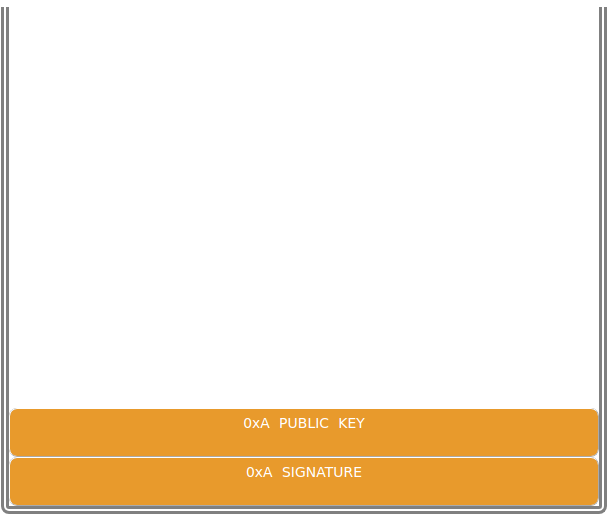
\includegraphics[scale=0.35]{images/script/p2pkh/1.png}
\captionof{figure}{Stato iniziale dello stack.\label{fig:stackp2pkh01}}
\vspace{10pt}
\par}


Incontrato l’operatore OP\_DUP, viene eseguita la copia dell’ultimo valore inserito all’interno dello stack, cioè <A pubkey> come in Figura \ref{fig:stackp2pkh02}.

{\centering
\vspace{15pt}
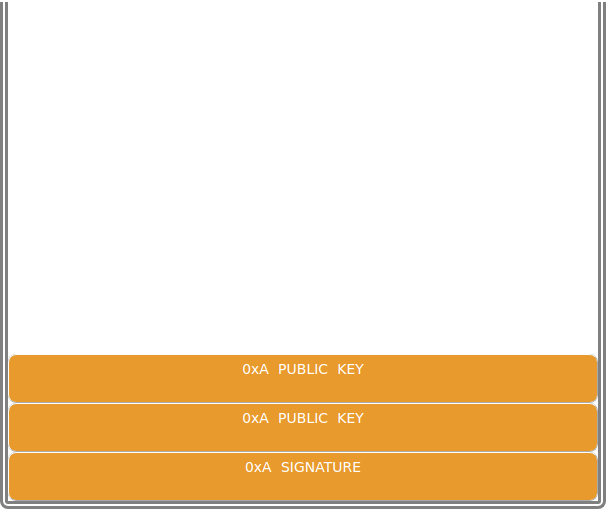
\includegraphics[scale=0.35]{images/script/p2pkh/2.png}
\captionof{figure}{Stato dello stack dopo l’esecuzione dell operatore OP\_DUP.\label{fig:stackp2pkh02}}
\vspace{10pt}
\par}

Incontrando l’operatore OP\_HASH160 viene calcolato l’hash dell’ultimo valore inserito ottenendo lo stato dello stack rappresentato in Figura \ref{fig:stackp2pkh03}.

{\centering
\vspace{15pt}
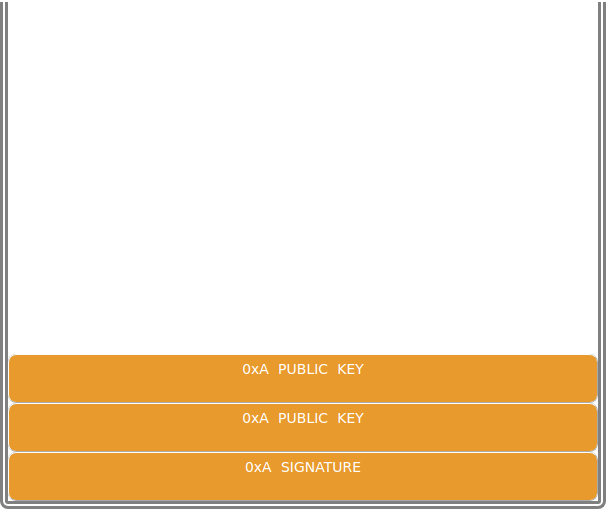
\includegraphics[scale=0.35]{images/script/p2pkh/2.png}
\captionof{figure}{Stato dello stack dopo l’esecuzione dell’operatore OP\_HASH160.\label{fig:stackp2pkh03}}
\vspace{10pt}
\par}

Viene quindi inserito all’interno dello stack l’hash della chiave pubblica atteso, cioè <A Pub Key Hash>, ottenendo lo stack rappresentato in Figura \ref{fig:stackp2pkh04}.

{\centering
\vspace{15pt}
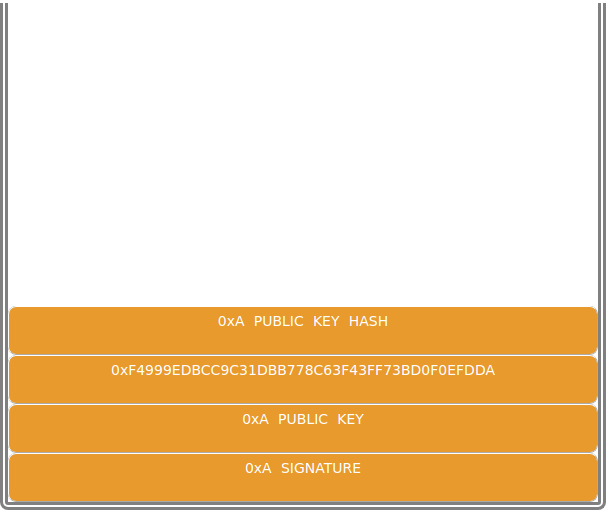
\includegraphics[scale=0.35]{images/script/p2pkh/4.png}
\captionof{figure}{Stato dello stack dopo l’inserimento della chiave pubblica attesa.\label{fig:stackp2pkh04}}
\vspace{10pt}
\par}

L ’operatore OP\_EQUALVERIFY a questo punto verifica che le chiavi pubbliche siano uguali; se lo sono, l’esecuzione continua altrimenti, termina con un risultato diverso da TRUE. Se l’esecuzione prosegue, viene valutato l’ultimo OP code cioè OP\_CHECKSIG, che ha il compito di verificare l’appartenenza della firma e della chiave pubblica alla medesima chiave privata A.

\subsection{P2PK}
Lo script {\it pay-to-public-key \/} è una forma di script più semplice del precedente, perché non viene applicato l’hash alla chiave pubblica e, quindi, l’indirizzo del ricevente è memorizzato nella transazione; per bloccare questo script si necessita solo della firma, il che fa sì che lo stack si semplifichi come segue:
\begin{lstlisting}[language=bitcoinscript, caption={P2PK Script completo.}]
<A Signature>
<A Public Key > OP_CHECKSIG
\end{lstlisting}

Quando il programma viene eseguito, lo stack è popolato con i valori dello script di sblocco come illustrato in Figura \ref{fig:stackp2pk01}.

{\centering
\vspace{10pt}
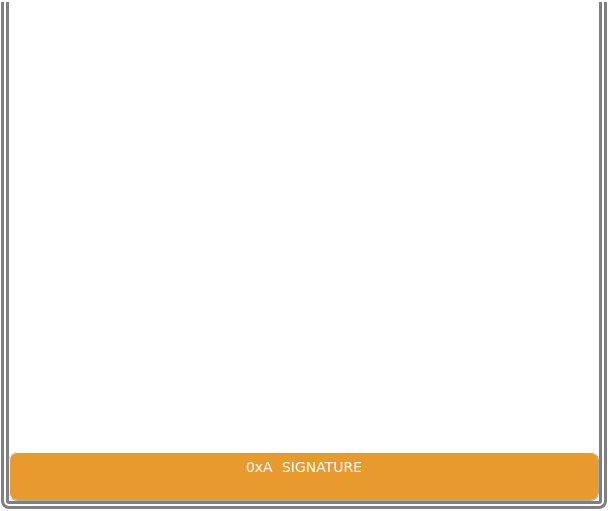
\includegraphics[scale=0.35]{images/script/p2pk/1.png}
\captionof{figure}{Stato dello stack dopo l’inserimento dello scriptSig.\label{fig:stackp2pk01}}
\vspace{10pt}
\par}

Nel passo successivo la chiave pubblica viene inserita nello stack, come rappresentato dalla Figura \ref{fig:stackp2pk02}.

{\centering
\vspace{10pt}
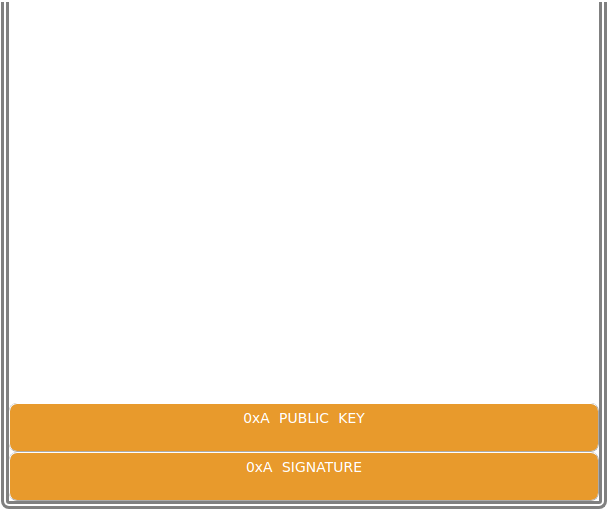
\includegraphics[scale=0.35]{images/script/p2pk/2.png}
\captionof{figure}{Stato dello stack dopo l’inserimento del <public key>.\label{fig:stackp2pk02}}
\vspace{10pt}
\par}

Avviene quindi la verifica tra firma e chiave pubblica con l’operatore OP\_CHECKSIG e, se  l’operatore ha come risultato TRUE, allora la transazione è sbloccabile con lo script di sblocco inserito.\newline
Lo script P2PK, oltre ad essere uno script semplice, viene considerato dagli sviluppatori un errore di implementazione originale, perché non contiene un indirizzo Bitcoin ma contiene la reale chiave pubblica derivata dall’algoritmo di curva ellittica, motivo per cui nell'agosto 2019 da uno script P2PK non è più possibile ricavare un indirizzo Bitcoin tramite il client ufficiale. In Figura \ref{fig:examplep2pkbuild} viene mostrata la differenza del processo di creazione tra uno script P2PK e uno script P2PKH.

{\centering
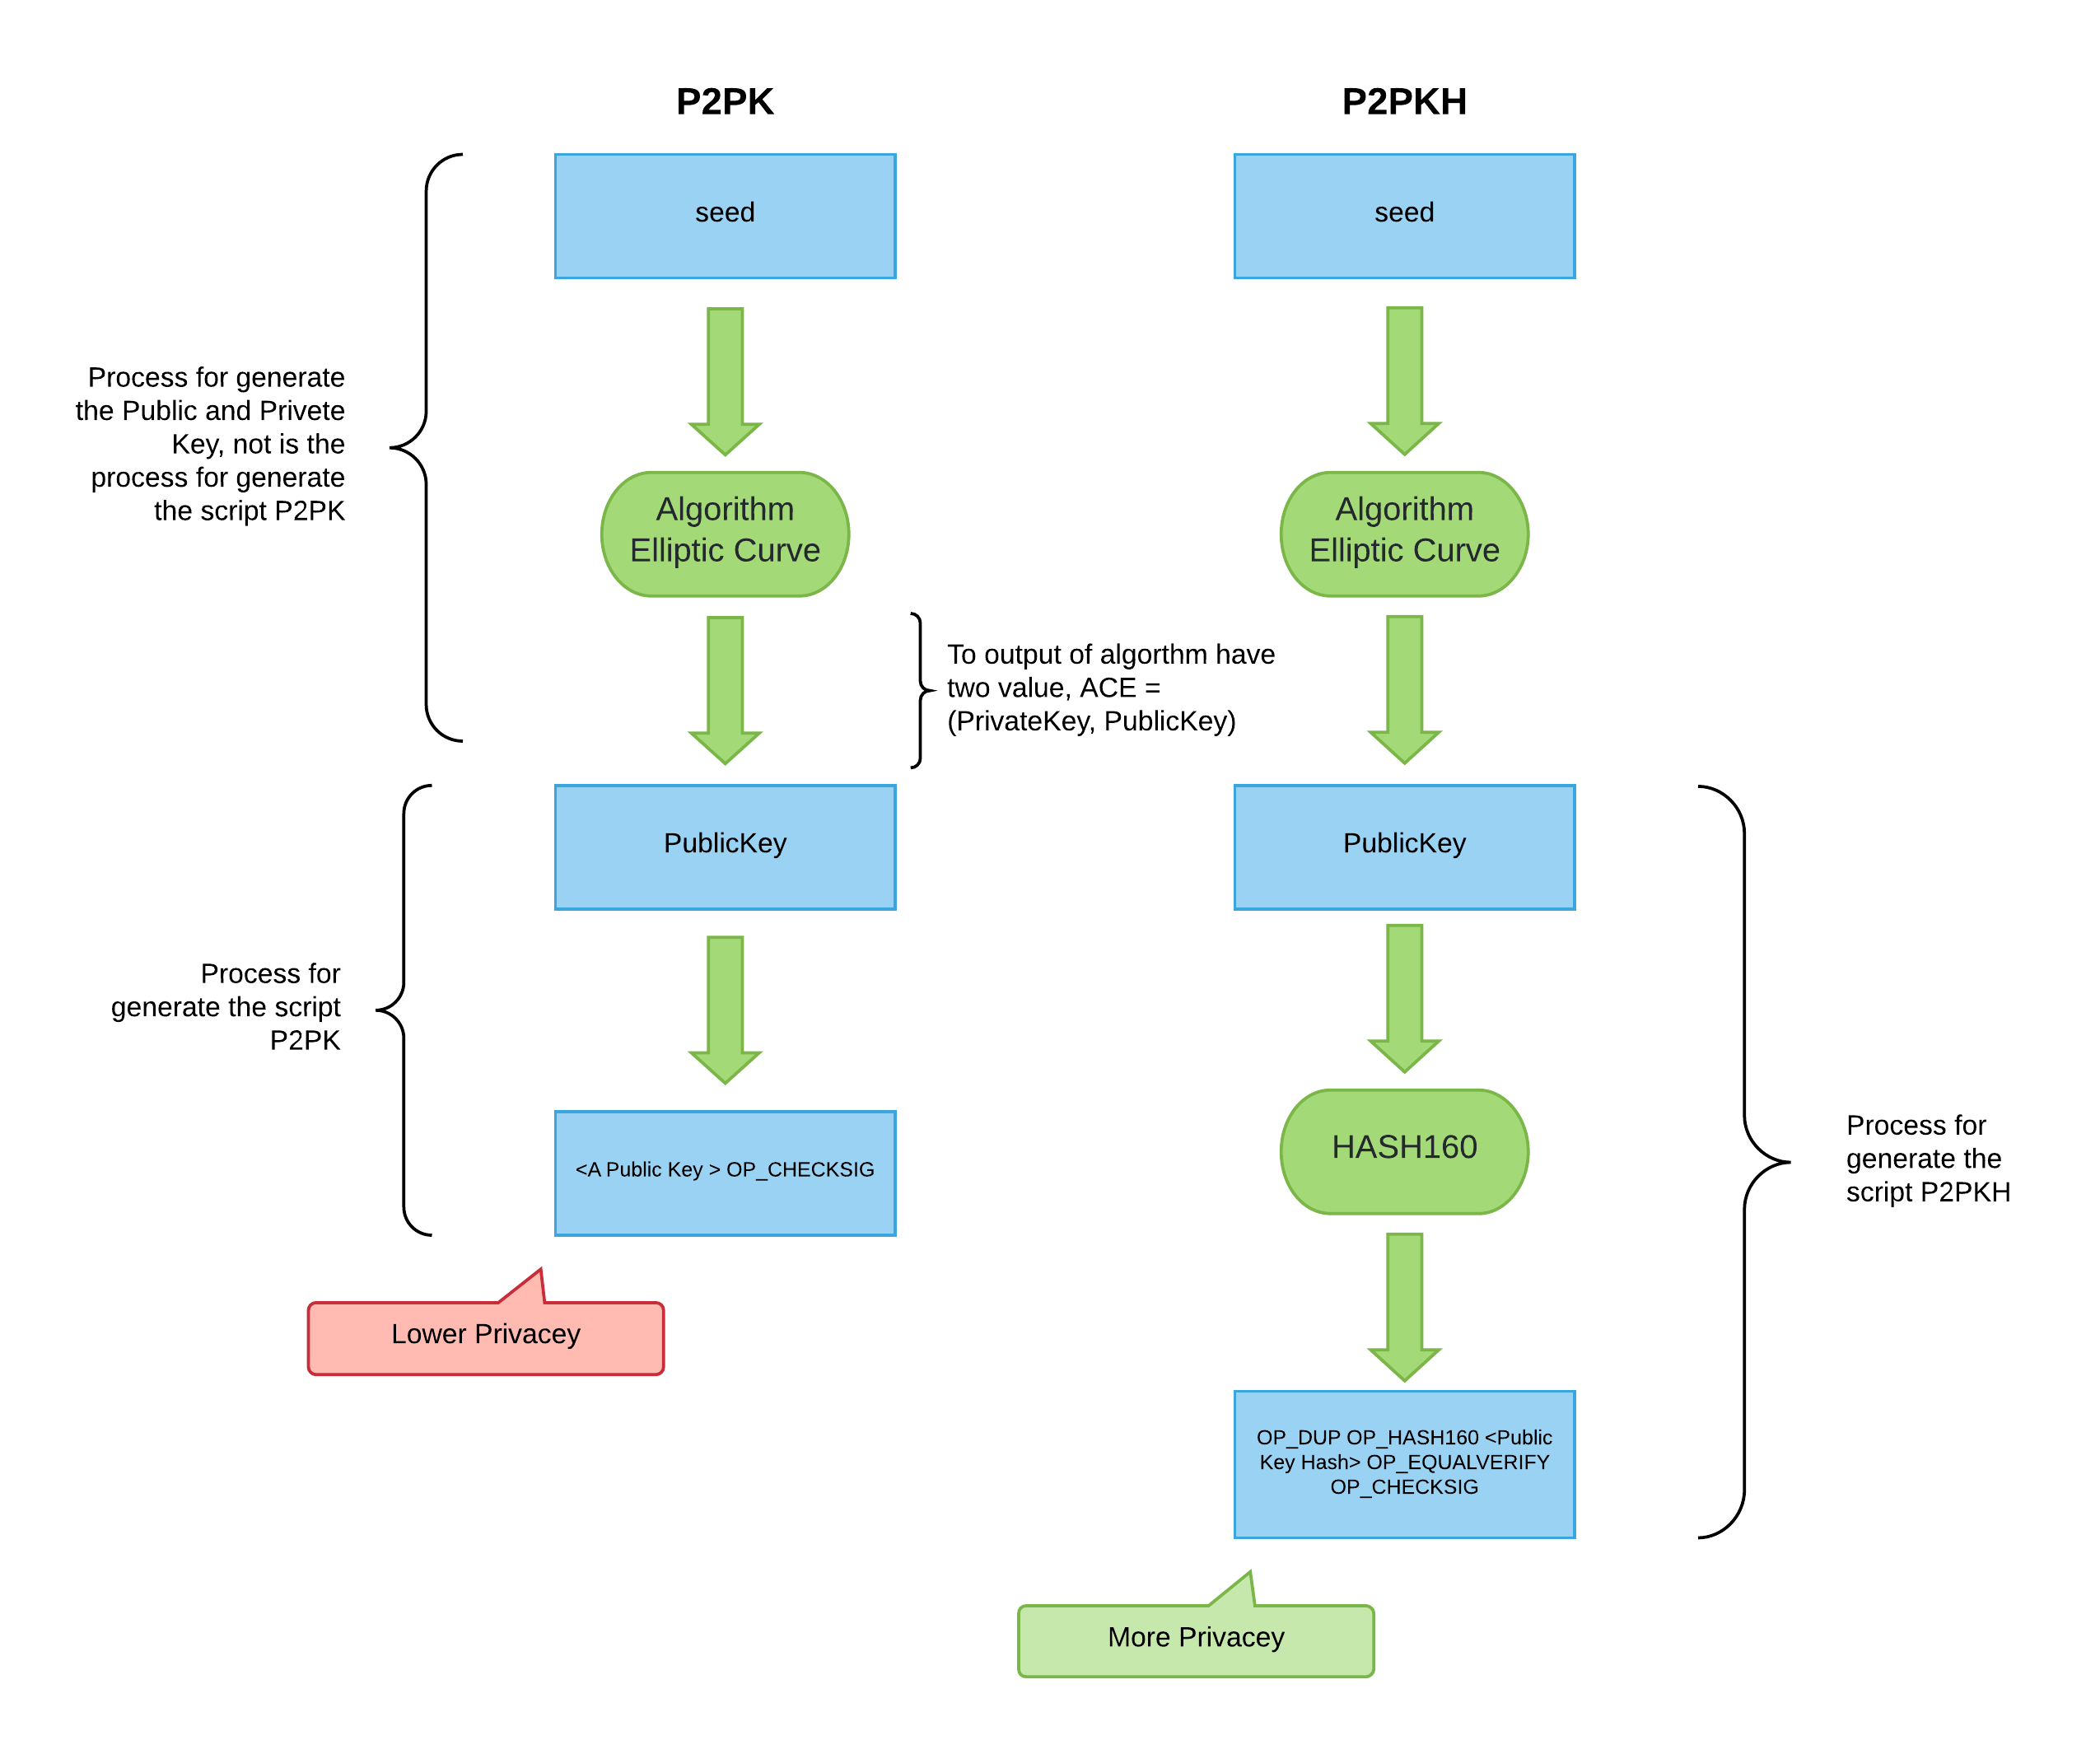
\includegraphics[scale=0.10]{images/proccessBuildP2PK.png}
\captionof{figure}{Rappresentazione del processo di creazione dello script P2PK e P2PKH.\label{fig:examplep2pkbuild}}
\par}

\subsection{P2MS}
\label{sec:p2msbitcoin}
Gli script {\it pay-to-multisignature} definiscono una condizione M:N (molti a molti) dove M è il numero minimo di firme necessarie per verificare lo script di blocco e N è il numero totale di chiavi pubbliche.
Il numero massimo di combinazioni ammesse per uno script P2MS è 15:15, ma solo le combinazioni rientranti nell’intervallo 3:3 sono considerate standard; tutte le restanti combinazioni verranno considerate come non standard.
Un esempio di script P2MS 2:3 è il seguente:

\begin{lstlisting}[language=bitcoinscript, caption={Script P2MS completo.}]
OP_0 <A Signature> <B Signature>
OP_2 <Public key A> <Public key B> <Public key C> OP_3 OP_CHECKMULTISIG
\end{lstlisting}
In questo esempio OP\_0 funge da segnaposto per un bug nell’implementazione di OP\_CHE\-CK\-MULTI\-SIG, il cui unico scopo è quello di aggirare un bug che è diventato accidentalmente una regola di consenso.

Lo stack inizialmente verrà popolato con i valori dello script di sblocco; la presenza dell’operatore OP\_0 implica che lo stack sia vuoto quando lo si incontra. Lo stato dello stack è rappresentato dalla Figura \ref{fig:stackmultsing01}.

{\centering
\vspace{15pt}
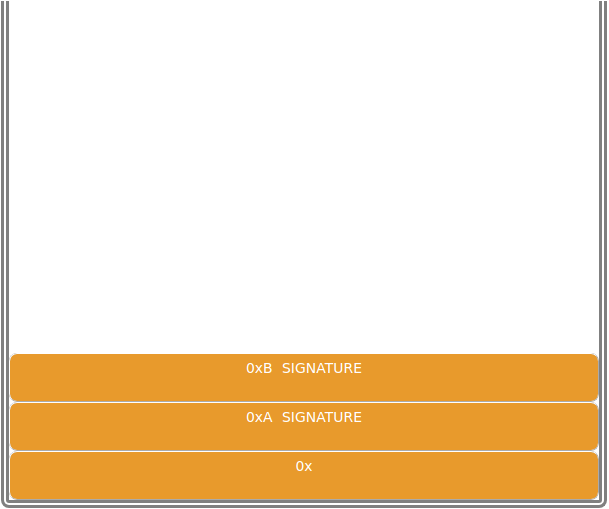
\includegraphics[scale=0.35]{images/script/multisig/1.png}
\captionof{figure}{Stato dello stack dopo l’inserimento dello scriptSig nello stack.\label{fig:stackmultsing01}}
\vspace{10pt}
\par}

L’operatore OP\_2 verifica che nello stack ci siano 2 elementi, successivamente vengono inserite le tre chiavi pubbliche, ottenendo così uno stato come in Figura \ref{fig:stackmultsing02}.

{\centering
\vspace{15pt}
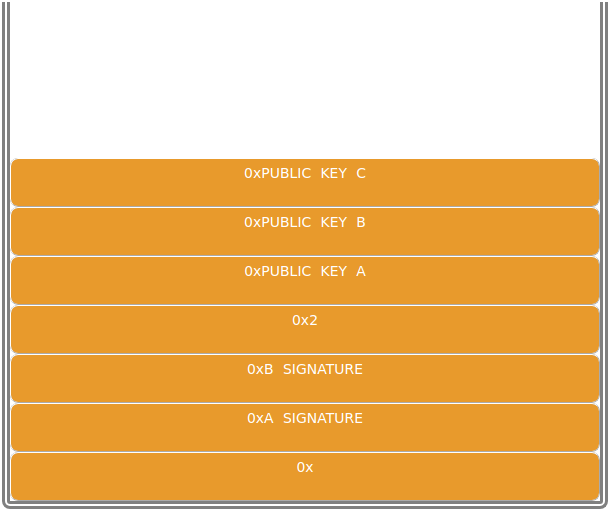
\includegraphics[scale=0.35]{images/script/multisig/2.png}
\captionof{figure}{Stato dello stack dopo la verifica con OP\_2 e l’inserimento nello stack delle chiavi pubbliche.\label{fig:stackmultsing02}}
\vspace{10pt}
\par}

Infine le firme vengono verificate con le chiavi pubbliche mediante l’operatore OP\_CHECK\-MULTI\-SIG in maniera iterativa, cioè la prima firma viene confrontata con tutte le chiavi pubbliche e l’azione si ripete per tutte le firme inserite, come in Figura \ref{fig:stackmultsing03}.

{\centering
\vspace{15pt}
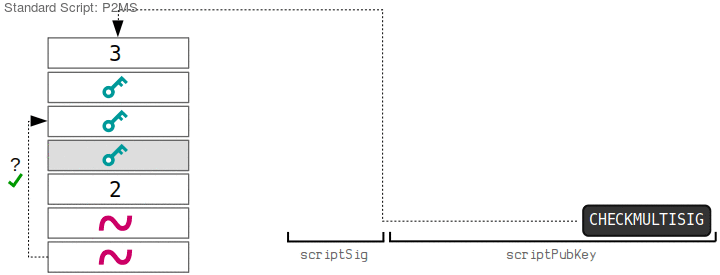
\includegraphics[scale=0.35]{images/script/multisig/3.png}
\captionof{figure}{Esecuzione dell’operatore OP\_CHECKMULTISIG per la verifica delle chiavi \cite{learnmeabitcoin:p2ms}.\label{fig:stackmultsing03}}
\vspace{10pt}
\par}

\subsection{P2SH}
Lo script {\it pay-to-script-hash \/} venne introdotto nel 2012, per semplificare l’uso degli script in transazioni complesse: infatti molto spesso accade di avere script molto grandi, come uno script P2MS 14:15, il che comporta un aumento della complessità dello script di sblocco; la motivazione dell’introduzione dello script P2SH è stata la semplificazione di quest’ultimo, come se fosse un normale pagamento ad un indirizzo Bitcoin.
Questa nuova tipologia semplifica notevolmente lo script di blocco, perché sarà popolato solo dal suo hash, a discapito però dell’aggiunta di una copia dello script di blocco all’interno dello script di sblocco. Si consideri, ad esempio il seguente script P2SH:

\lstinputlisting[label=code:p2shnokey, caption={Script P2SH completo.}]{code/script/p2sh-without-key.btcs}

In questo esempio lo script P2SH (Codice \ref{code:p2shnokey}) completo viene composto dal seguente script di sblocco:
\begin{lstlisting}[language=bitcoinscript, label={code:p2shunlock}, caption={Script P2SH di sblocco.}]
OP_0 <A Signature> <B Signature> OP_2 <Public key A> <Public key B>
<Public key C> OP_3 OP_CHECKMULTISIG
\end{lstlisting}

Esso conterrà anche lo script di blocco, conosciuto, in questo caso, come script di riscatto ({\it redeemScript\/}). Quindi nello script di sblocco si possono distinguere:
\begin{itemize}
  \item {\bf <signature>\/}: Composto da <A Signature> <B Signature>.
  \item {\bf <redeemScript>\/}: Composto da OP\_2 <Public key A> <Public key B> <Public key C> OP\_3 OP\_CHECKMULTISIG.
\end{itemize}

Diversamente, lo script di blocco si semplifica come nell’esempio seguente:
\begin{lstlisting}[language=bitcoinscript, label={code:p2shlock}, caption={Script P2SH di blocco.}]
OP_HASH160 <ScriptSig Hash> OP_EQUAL
\end{lstlisting}

L’esecuzione del Codice \ref{code:p2shnokey} si suddivide in due passaggi:

\begin{enumerate}
  \item Viene valutato lo script di sblocco come descritto nella Sezione \ref{sec:p2msbitcoin}.
  \item Viene verificato l'hash ricavato dallo script di riscatto con l’hash inserito all’interno dello script di blocco.
\end{enumerate}

Il passo 1 dell’esecuzione consiste nella valutazione dello script di sblocco come un normale script P2MS, lasciando invariato lo stato di esecuzione dello stack.
Il passaggio 2, invece, viene eseguito solo se l’esecuzione precedente restituisce TRUE; nel caso di  script P2MS validi l’esecuzione prosegue con una copia dello stack all’interno di un nuovo stack popolato solo dal redeemScript.

Lo stato del nuovo stack viene popolato con i dati relativi allo script di riscatto come mostrato in Figura \ref{fig:stackp2sh01}.

{\centering
\vspace{15pt}
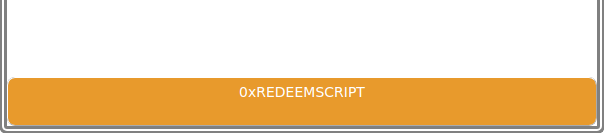
\includegraphics[scale=0.35]{images/script/p2sh/1.png}
\captionof{figure}{Stato dello stack dopo l’esecuzione dello ScriptSig come script P2MS.\label{fig:stackp2sh01}}
\vspace{10pt}
\par}

Viene valutato l’operatore OP\_HASH160, che esegue l’hash del redeemScript e porta lo  stack nello stato riportato in Figura \ref{fig:stackp2sh02}.

{\centering
\vspace{15pt}
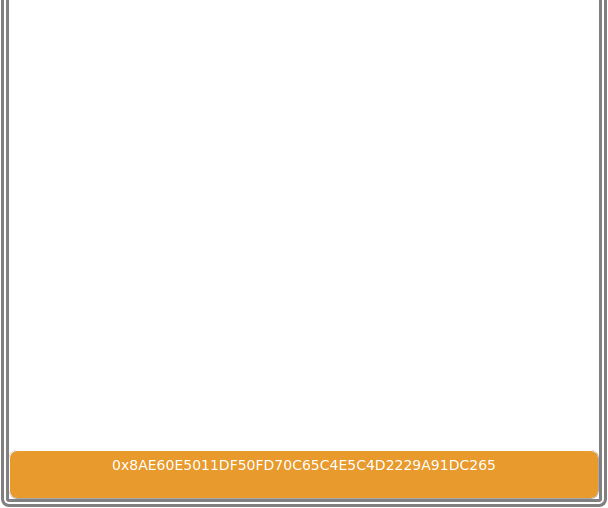
\includegraphics[scale=0.35]{images/script/p2sh/2.png}
\captionof{figure}{Stato dello stack dopo l’esecuzione dell’operatore OP\_HASH160.\label{fig:stackp2sh02}}
\vspace{10pt}
\par}

Come ultimo passaggio viene inserito l’hash atteso contenuto nello script di sblocco, ottenendo lo stato dello stack mostrato in Figura \ref{fig:stackp2sh03}.

{\centering
\vspace{15pt}
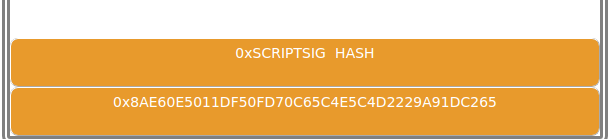
\includegraphics[scale=0.35]{images/script/p2sh/3.png}
\captionof{figure}{Stato dello stack dopo l’inserimento dell’hash atteso.\label{fig:stackp2sh03}}
\vspace{10pt}
\par}

Infine, eseguendo l’operatore OP\_EQUAL viene verificata l’uguaglianza degli hash; l’esito di tale confronto definisce il futuro della transazione.

Nell'implementazione del P2SH è stata aggiunta un’altra importante caratteristica cioè la possibilità di codificare un hash di script come un indirizzo Bitcoin attraverso l’utilizzo della codifica Base58; l’indirizzo ricavato è conosciuto anche come indirizzo P2SH, con l’unica differenza che quest'ultimo inizierà con il numero 3 per convenzione.

Un esempio di indirizzo Bitcoin P2SH:

\begin{lstlisting}[language=bitcoinscript, caption={Indirizzo Bitcoin P2SH.}]
3EBe7iCt2vhC9gqw9UdeaudjYkbfpq3b8c
\end{lstlisting}

Un'indirizzo primitivo Bitcoin:

\begin{lstlisting}[language=bitcoinscript, caption={Indirizzo Bitcoin primitivo.}]
1A1zP1eP5QGefi2DMPTfTL5SLmv7DivfNa
\end{lstlisting}

Attraverso l’indirizzo Bitcoin calcolato dallo script, si può riscrivere il Codice \ref{code:p2shlock} come segue:
\begin{lstlisting}[language=bitcoinscript, label={code:p2shlockwithkey}, caption={Script P2SH di blocco con Indirizzo Bitcoin P2SH.}]
OP_HASH160 <P2SH key> OP_EQUAL
\end{lstlisting}

Quindi lo script completo diventa:

\lstinputlisting[label=code:p2shkey, caption={Script P2SH completo con indirizzo Bitcoin P2SH.}]{code/script/p2sh-with-key.btcs}

L’esecuzione del Codice \ref{code:p2shkey}, che contiene un indirizzo Bitcoin P2SH al posto del hash dello script, non cambia, perché la chiave ricavata dallo script viene decodificata nel suo hash risultante, così da lasciare la sua esecuzione invariata.
Bitcoin utilizza la convenzione dell'id wallet solo per una semplificazione per l'occhio umano, ma non necessita di queste informazioni per compiere le sue ordinarie operazioni; inoltre gli script P2SH e quindi gli script P2MS (in particolare script P2MS 2:2) vengono utilizzati estensivamente per la creazione e la gestione di canali all’interno della tecnologia {\it Lightning network\/}, che aumentano drasticamente la velocità delle transazioni con Bitcoin, utilizzando un protocollo {\it off-chain\/}.

\subsection{Transazioni null data (OP\_RETURN)}
La blockchain di Bitcoin e, più in generale, le tecnologie blockchain hanno potenziali usi ben oltre i pagamenti. Molti sviluppatori hanno tentato di utilizzare Bitcoin script, per sfruttare la sicurezza e la resilienza del sistema, per applicazioni quali servizi notarili digitali, certificati azionari e {\it smart contract\/}.

I primi tentativi di utilizzare il linguaggio di script di Bitcoin per questi scopi hanno comportato la creazione di output di transazioni, che registravano dati sulla blockchain; nella versione 0.9 di Bitcoin core del 2014, è stato aggiunto un nuovo tipo di operatore chiamato OP\_RETURN che marca la transazione come non correlata ad un movimento di bitcoin, ma ad un'archiviazione di dati. Questo operatore ha permesso ai miner di identificare la transazione e decidere se validarla o meno, considerando il problema che, archiviando una transazione con uno script non valido, oltre a creare un UTXO non spendibile, lo spazio richiesto della blockchain di bitcoin sarebbe aumentato, aumentando quindi anche le commissioni richieste dal miner.
Per aggirare questo problema, il team di sviluppo decise di limitare la porzione di dati a 80 byte.

\begin{lstlisting}[language=bitcoinscript, label={code:nulldata}, caption={Uso dell'operatore OP\_RETURN.}]
OP_RETURN <data>
\end{lstlisting}

Lo script precedente non fa altro che marcare il campo <data> come dati grezzi che non riguardano una transazione; infatti la semantica dell’operatore OP\_RETURN marca la transazione come invalida, quindi i dati non vengono valutati.

\section{Mining}
\label{sec:miningbitcoin}

Il processo di Mining si avvale dell’algoritmo di Proof of Work, per generare nuovi bitcoin e proteggere la rete da attacchi di malintenzionati, come ad esempio la pubblicazione di un blocco non valido o la modifica di una transazione all’interno di un blocco.\newline
Bitcoin esegue la validazione delle transazioni in media ogni 10 minuti ed esse vengono considerate valide solo quando il blocco che le contiene viene accodato alla catena ufficiale; ogni transazione può includere all’interno un valore di bitcoin che equivale ad una tassa indirizzata al miner per ricompensa del lavoro svolto, il quale può scegliere di dare precedenza a transazioni con una commissione maggiore di un quantitativo di bitcoin a loro scelta.\newline
Bitcoin stabilisce un processo di creazione di nuova moneta decrescente e limitato: infatti impone un limite superiore massimo di \(2.1 * 10^{15} \) bitcoin; il valore creato dai miner si dimezza ogni 210.000 blocchi, in media ogni 4 anni.
La creazione di bitcoin iniziò con un ammontare pari a 50 bitcoin per blocco nel gennaio 2009 e si dimezzò a 25 bitcoin nel novembre 2012, stimando così l’emissione completa di tutti i bitcoin disponibili nel 2140; al termine dell’emissione, il guadagno di ogni miner sarà esclusivamente il valore della commissione.
L’utilizzo dell protocollo Proof of Work, che è per sua natura {\it CPU-bound\/}, nel corso degli anni, con l’aumentare della competitività nel settore del mining di bitcoin, portò ad un aumento esponenziale della potenza di hashing, subendo così un cambiamento radicale della tecnologia utilizzata: si è passati da comuni CPU a componenti appositi per il calcolo della funzione hash del tipo FPGA (\emph{mining and field programmable gate array}).\footnote{Nel 2014, l'energia consumata dalla rete Bitcoin era pari al consumo di elettricità dell'Irlanda (O'Dwyer e Malone, 2014)}
L’aumento della potenza di hashing (Figura \ref{fig:hashrate}) portò anche ad un aumento della difficoltà di estrazione di un blocco conosciuta come difficoltà metrica (Figura \ref{fig:metrix}).

{\centering
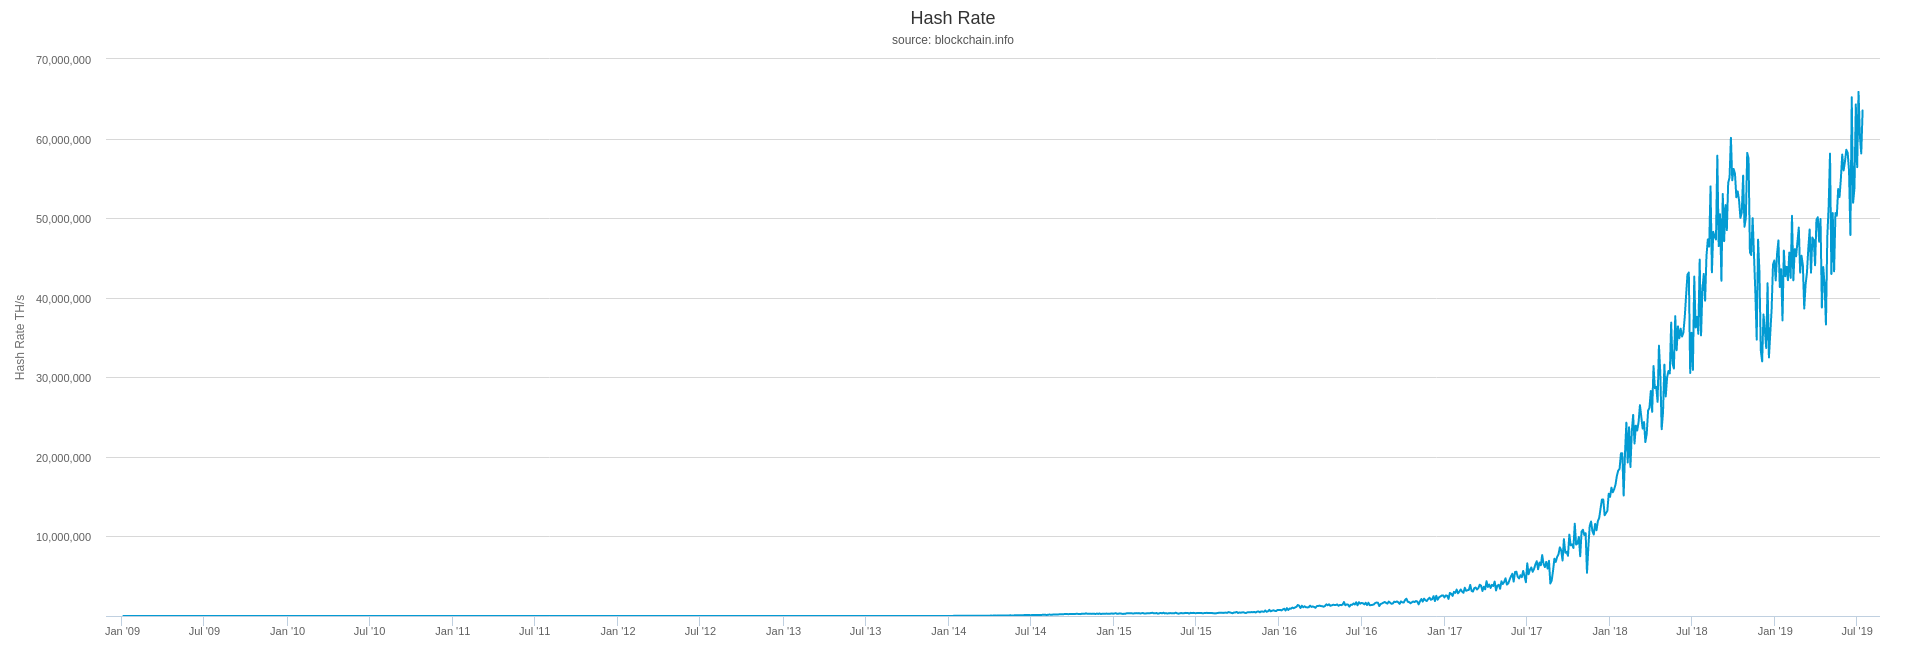
\includegraphics[scale=0.2]{images/hash-rate.png}
\captionof{figure}{Grafico della crescita della potenza di hashing in data 28/09/2019. Fonte: blockchain.com.\label{fig:hashrate}}
\par}

{\centering
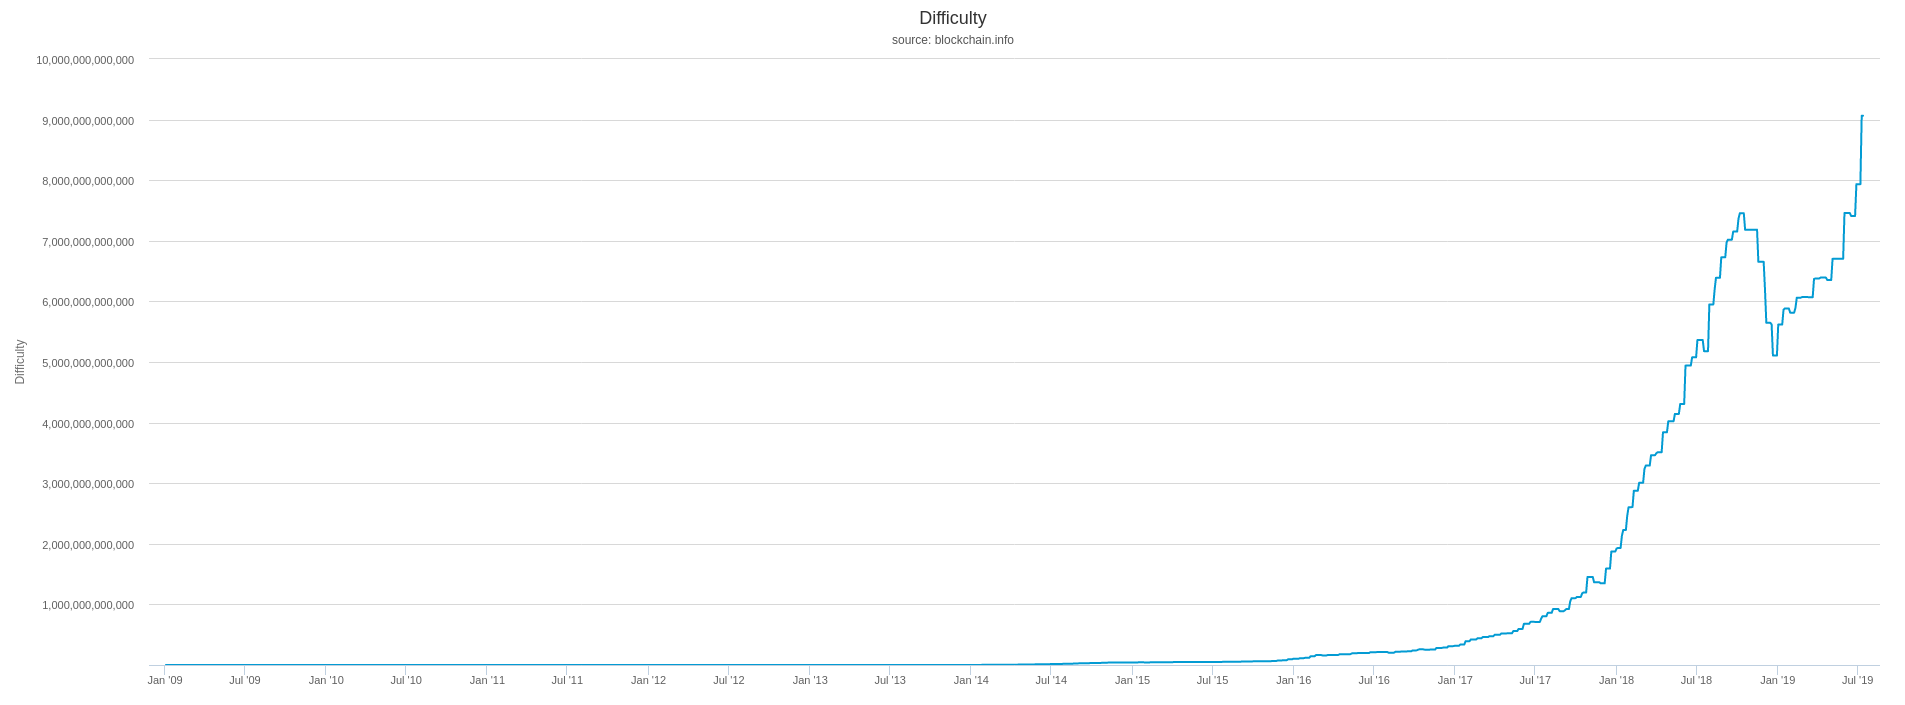
\includegraphics[scale=0.2]{images/difficulty.png}
\captionof{figure}{Grafico della crescita della difficoltà metrica in data 28/09/2019. Fonte: blockchain.com.\label{fig:metrix}}
\par}

\chapter{Bitcoin core}
\label{chap:bitcoin core}

\section{Introduzione}\label{sec:introduzionebitcoincore}

Bitcoin core è il successore della versione rilasciata da Satoshi Nakamoto ora conosciuta come “satoshi client”; attualmente è il client di riferimento del protocollo Bitcoin.
Bitcoin core è un progetto open-source scritto in C++, il cui codice sorgente risiede attualmente su Github sotto licenza MIT e viene sviluppato da una comunità aperta di volontari; esso costituisce una riscrittura quasi completa della versione 0.1.0 del client rilasciato da Satoshi Nakamoto.

\section{Blocchi}
\label{sec:blocchibitcoincore}

Così come le transazioni, il blocco viene definito attraverso una struttura dati: una volta creato e pubblicato un blocco, viene serializzato all’interno di un flat file, mantenendo i riferimenti necessari per eseguire la deserializzazione all’interno del database LevelDB di Google; le informazioni necessarie del blocco vengono contenute all’interno una struttura chiamata BlockHeader e la dimensione della struttura da deserializzare è pari a 80 byte, come rappresentato in Tabella \ref{tab:blockheaderbitcoinc}

\begin{table}
       \centering\small
           \begin{tabular}{|c|c|}
               \hline
                 \multicolumn{2}{|c|}{\textbf{BlockHeader}} \\
                 %\cmidrule(lr){1-2}
                 \hline
                 \multicolumn{1}{|c|}{Type} & \multicolumn{1}{c|}{Name} \\
               \hline \hline
               $int32\_t$ & nVersion   \\
               \hline
               $uint256$ & hashPrevBlock \\
                \hline
               $uint256$ & hashMerkleRoot \\
                \hline
               $uint32\_t$ & nTime \\
                \hline
               $uint32\_t$ & nBits \\
                \hline
               $uint32\_t$ & nNonce \\
               \hline
       \end{tabular}
       \caption{Struttura di un block header in Bitcoin core.\label{tab:blockheaderbitcoinc}}
   \end{table}


\begin{itemize}
  \item {\bf nVersion\/}: Identifica le regole seguite dal blocco; fino ad ora si possono identificare 4 versioni, tutte introdotte attraverso dei soft-fork.
  \item {\bf hashPrevBlock e hashMerkleRoot\/}: Appartengono ad un tipo di dato non primitivo del C++, ma ad un tipo definito da Bitcoin core. Rappresentano una struttura dati da 32 byte in cui vengono memorizzati l’hash del blocco precedente (in {\tt{hashPrevBlock}}) e la radice del Merkle Tree (in {\tt{hashMerkleRoot}}); queste ultime garantiscono che il blocco non possa in nessun modo essere modificato, senza alterare l’intestazione del blocco.
  \item {\bf nTime\/}: Valore che rappresenta un’epoca Unix e indica il momento in cui il miner ha iniziato ad eseguire la Proof of Work per convalidare il blocco.
  \item {\bf nBits\/}: Un intero a 8 byte, che rappresenta il target di difficoltà dell’algoritmo di PoW del blocco.
  \item {\bf nNonce\/}: Valore intero a 8 byte usato per contenere il valore generato dall’algoritmo di PoW.
\end{itemize}

Il blocco, oltre a contenere l’intestazione, contiene ulteriori informazioni riguardo la sua dimensione e la rete di appartenenza: infatti il client Bitcoin può essere eseguito anche in modalità testnet, in cui vengono testate le nuove versioni del software prima del rilascio ufficiale.
La struttura finale del blocco, nella version attuale, può essere rappresentata nel modo indicato in Tabella \ref{tab:blockbitcoinc}

\begin{table}
       \centering\small
           \begin{tabular}{|c|c|}
               \hline
                 \multicolumn{2}{|c|}{\textbf{Block}} \\
                 %\cmidrule(lr){1-2}
                 \hline
                 \multicolumn{1}{|c|}{Type} & \multicolumn{1}{c|}{Name} \\
               \hline \hline
               $int32\_t$ & magicNumber   \\
               \hline
               $int32\_t$ & blockSize \\
               \hline
               BlockHeader & blockHeader \\
               \hline
               CompactSize & numberTx \\
               \hline
               vector<RawTransaction> & transactions \\
               \hline
       \end{tabular}
       \caption{Struttura di un blocco in Bitcoin core.\label{tab:blockbitcoinc}}
   \end{table}

\begin{itemize}
  \setlength\itemsep{1em}
  \item {\bf magicNumber\/}: Rappresenta una signature per la struttura dati e non è qualcosa di specifico per Bitcoin; il numero magico viene usato, infatti, nell’informatica per i file e i protocolli, per semplificare notevolmente il riconoscimento del file o della struttura dati: ad esempio il numero magico per un file png è 89504E470D0A1A0A, mentre il numero magico di bitcoin per la rete principale è rappresentato da 0xD9B4BEF9.
  \item {\bf numberTx\/}: Il valore rappresenta il numero di transazioni contenute all'interno del blocco e viene serializzato usando un metodo simile alla tecnica di memorizzazione dei record a lunghezza variabile all’interno di un database relazionale; in Bitcoin core viene rappresentato attraverso un tipo di dato che porta il nome di VarInt (intero variabile) e questo valore occupa da 1 a 9 byte di spazio.
  Il client utilizza VarInt all’interno di LevelDB, ma utilizza il tipo di dato CompactSize rilasciato nella versione 0.1.0 di Satoshi per la serializzazione all’interno del file.
\end{itemize}

\section{Transazioni}
\label{sec:transazionibitcoincore}
Come descritto nel Capitolo di \ref{sec:transazioniBitcoin}, esse rappresentano l’elemento fulcro del sistema; nel corso degli anni, gli sviluppatori di Bitcoin core hanno dovuto confrontarsi con problemi nell’implementazione originale delle transazioni: uno di essi è conosciuto come problema di malleabilità.
La malleabilità di una transizione consisteva nella possibilità di alterare l’identificativo della transizione (txId) durante il processo di verifica senza invalidarla. La motivazione dell’alterazione era dovuta alla possibilità di modificare le firme nello script di sblocco (scriptSig) senza cambiare il loro significato; quindi per il modo in cui viene calcolato l’hash della transizione, questa alterazione comportava inevitabilmente l’alterazione dell’hash, portando all’interno del protocollo le seguenti problematiche:
\begin{itemize}
  \item Il mittente non può più riconoscere la sua transazione dopo che essa è stata modificata.
  \item Le transazioni modificate sono effettivamente riconosciute come doppie spese, perché il mittente, non riuscendo più a riconoscere la sua transazione di input creata in precedenza, si ritroverà i bitcoin invariati e potrà spenderli una seconda volta.
  Questo problema non grava sul mittente, ma sull’intero sistema Bitcoin: ad esempio le transazioni che non vengono riconosciute dal mittente saranno sepolte all’interno della blockchain perché mai nessuno sarà in grado di spenderle.
\end{itemize}

Nel 2016 la community arrivò ad una soluzione tramite un soft-fork, che introdusse notevoli cambiamenti strutturali, risolvendo tutti i problemi relativi alla malleabilità di una transazione. Questo aggiornamento venne chiamato \say{Segregated Witness} e suddivise le transazioni in diverse parti, che possono essere gestite separatamente, sostituì le firme digitali con un segnaposto all’interno delle transazioni spostando le vere firme in una struttura dati differente. Questa soluzione non esclude però la possibilità che una transazione non sia malleabile, ma esclude una modifica dell’hash durante la verifica, poiché i dati utilizzati per il calcolo sono contenuti all’interno di uno spazio protetto; da qui nasce il nome Segregated Witness.

La struttura riportata in Figura \ref{tab:rawtxbitcoinc} rappresenta la struttura delle transazioni:

\begin{table}
       \centering\small
           \begin{tabular}{|c|c|}
               \hline
                 \multicolumn{2}{|c|}{\textbf{RawTransaction}} \\
                 %\cmidrule(lr){1-2}
                 \hline
                 \multicolumn{1}{|c|}{Type} & \multicolumn{1}{c|}{Name} \\
               \hline \hline
               $int32\_t$ & version   \\
               \hline
               $uint8\_t$ & marker \\
               \hline
               $uint8\_t$ & flag \\
               \hline
               CompactSize & numberTxIn \\
               \hline
               vector<TransactionInput> & transactionsInput \\
               \hline
               CompactSize & numberTxOut \\
               \hline
               vector<TransactionOutput> & transactionsOutput \\
               \hline
               vector<TransactionWitness> & transactionsWitness \\
               \hline
       \end{tabular}
       \caption{Struttura della transazione dopo l’aggiornamento al Segregated witness.\label{tab:rawtxbitcoinc}}
   \end{table}

\begin{itemize}
  \item {\bf marker e flag\/}: Sono valori interi a 1 byte che fungono da identificativo per una transazione conforme al formato Segregated Witness (SegWit); per i wallet non conformi al SegWit la transazione risulterà non valida, perché identifica una transazione con 0 input e 1 output.
  \item {\bf transactionsWitness\/}: Questa lista non è preceduta da una dimensione perché la singola transazione witness ha senso solo se esiste un input correlato, quindi la dimensione di questa lista è uguale alla dimensione della lista delle transazioni di input.
\end{itemize}

Le transazioni di input sono definite tramite una struttura rappresentata dalla Tabella \ref{tab:inputtxbitcoinc}.

\begin{table}
       \centering\small
           \begin{tabular}{|c|c|}
               \hline
                 \multicolumn{2}{|c|}{\textbf{TransactionInput}} \\
                % \cmidrule(lr){1-2}
                \hline \hline
                 \multicolumn{1}{|c|}{Type} & \multicolumn{1}{c|}{Name} \\
               \hline
               Outpoint & outpoint   \\
               \hline
               CScript & scriptSig \\
               \hline
               $uint32\_t$ & nSequence \\
               \hline
       \end{tabular}
       \caption{La struttura della transazione input all’interno di Bitcoin core.\label{tab:inputtxbitcoinc}}
   \end{table}

\begin{itemize}
  \item {\bf nSequence\/}:  Il valore viene utilizzato per esprimere il timelock relativo a livello di transazione (argomento trattato nel Capitolo \ref{sec:bitcoinScriptBitcoinCore}).
  \item {\bf scriptSig\/}: Rappresenta la condizione di sblocco espressa dalla transazione sotto forma di script.
\end{itemize}

Il tipo di dato Outpoint utilizzato nella transazione di input contiene le informazioni necessarie per identificare la transazione di output contenuta in una transazione precedente. La Tabella \ref{tab:outpointbitcoinc} ne descrive la struttura.


\begin{table}
       \centering\small
           \begin{tabular}{|c|c|}
               \hline
                 \multicolumn{2}{|c|}{\textbf{Outpoint}} \\
                % \cmidrule(lr){1-2}
                \hline \hline
                 \multicolumn{1}{|c|}{Type} & \multicolumn{1}{c|}{Name} \\
               \hline
               $uint256$ & hash   \\
               \hline
               $uint32\_t$ & index \\
              \hline
       \end{tabular}
       \caption{Struttura del tipo di dato Outpoint di Bitcoin core.\label{tab:outpointbitcoinc}}
   \end{table}

\begin{itemize}
  \item {\bf hash\/}:  Rappresenta l’hash delle transazione precedente che contiene l’UTXO sbloccato dalla transazione di input che contiene outpoint.
  \item {\bf index\/}: Il valore indica l’indice della lista in cui è memorizzato l’UTXO nella transazione precedente.
\end{itemize}

La struttura della transazione di output contiene esclusivamente le informazione dello script di blocco e il valore di bitcoin (in satoshi); in Tabella \ref{tab:transactionOutput} viene illustrata la struttura dati corrispondente.

\begin{table}[H]
       \centering\small
           \begin{tabular}{|c|c|}
               \hline
                 \multicolumn{2}{|c|}{\textbf{TransactionOutput}} \\
                % \cmidrule(lr){1-2}
                \hline \hline
                 \multicolumn{1}{|c|}{Type} & \multicolumn{1}{c|}{Name} \\
               \hline
               $int64\_t$ & nValue   \\
               \hline
               CScript & scriptPubKey \\
               \hline
       \end{tabular}
       \caption{La struttura della transazione di output di Bitcoin core.\label{tab:transactionOutput}}
   \end{table}

\begin{itemize}
  \item {\bf nValue\/}: Rappresenta il valore di bitcoin (in satoshi) contenuti nella transazione.
  \item {\bf scriptPubKey\/}: Rappresenta la condizione di blocco espressa dalla transazione sotto forma di script.
\end{itemize}

La transazione Witness rappresenta la serializzazione di tutti i dati del testimone; in Tabella \ref{tab:witnesstxbitcoinc} viene illustrata la  struttura dati corrispondente.

\begin{table}[H]
       \centering\small
           \begin{tabular}{|c|c|}
               \hline
                 \multicolumn{2}{|c|}{\textbf{TransactionWitness}} \\
                 %\cmidrule(lr){1-2}
                 \hline
                 \multicolumn{1}{|c|}{Type} & \multicolumn{1}{c|}{Name} \\
               \hline \hline
               CompactSize & stackSize   \\
               \hline
               CScript & stack \\
               \hline
       \end{tabular}
       \caption{La struttura della serializzazione dei dati del testimone; in Bitcoin core questa struttura è chiamata CScriptWitness.\label{tab:witnesstxbitcoinc}}
   \end{table}

\begin{itemize}
  \item {\bf stackSize\/}: Il valore rappresenta il numero di script contenuti all’interno della transazione.
  \item {\bf stack\/}: Il valore contiene la lista di script per la singola transazione di input.
\end{itemize}
\leavevmode
\newline
Il tipo di dato CScript è un tipo di dato contenente le informazioni necessarie per lo script; la Tabella \ref{tab:scriptbitcoinc} ne descrive la struttura.


\begin{table}
       \centering\small
           \begin{tabular}{|c|c|}
               \hline
                 \multicolumn{2}{|c|}{\textbf{CScript}} \\
                 %\cmidrule(lr){1-2}
                 \hline
                 \multicolumn{1}{|c|}{Type} & \multicolumn{1}{c|}{Name} \\
               \hline \hline
               CompactSize & scriptSize   \\
               \hline
               vector<unsigned char> & script \\
               \hline
       \end{tabular}
       \caption{Struttura del tipi di dato CScript di Bitcoin core.\label{tab:scriptbitcoinc}}
   \end{table}

\begin{itemize}
  \item {\bf scriptSize\/}: Rappresenta la lunghezza in byte dello script, espressa tramite il tipo di dato CompactSize.
  \item {\bf script\/}: Rappresenta il vettore di byte dello script.
\end{itemize}
\leavevmode
%\newpage
\section{Bitcoin script}
\label{sec:bitcoinScriptBitcoinCore}

L’aggiornamento Segregated Witness comporta un notevole cambiamento anche sulla modalità di spesa degli UTXO; infatti tutti i tipi di transazione visti finora fanno riferimento allo script di sblocco, contenuto all’interno della transazione di input.
Con il nuovo aggiornamento lo script di sblocco viene spostato all’interno di una struttura al di fuori delle transazioni di input, chiamata \say{Transazione Witness} e mostrata in Tabella \ref{tab:rawtxbitcoinc}.
I dati relativi alle transazioni witness non contengono le informazioni di una reale transazione, bensì costituiscono uno spazio riservato per esprimere la condizione di sblocco.
Per sbloccare un UTXO con il Segregated Witness bisogna far riferimento allo script contenuto all’interno delle transazioni witness, come illustrato in Tabella \ref{tab:witnesstxbitcoinc} (che chiameremo script witness). Questa modifica nella spesa degli UTXO ha costretto Bitcoin script ad un soft fork: ogni script d’ora in poi conterrà un numero di versione all’inizio che permette l’identificazione del tipo di transazione; lo script inizierà con un numero di versione uguale a zero per identificare uno script Witness, rendendo la transazione interpretabile anche da wallet non abilitati al Segregated Witness. Attraverso questa soluzione la transazione risulta essere spendibile da chiunque.
Gli script P2PKH e P2SH con il testimone segregato si evolvono in P2WPKH e P2WSH

\subsection{P2WPKH}

Lo script {\it pay-to-witness-public-key-hash \/} si semplifica notevolmente rispetto allo script P2PKH: infatti lo script witness include la versione di verifica e l’hash della chiave pubblica come nello script  P2PKH,  ma in P2WPKH è chiamato “programma di controllo”, composto da 20 byte.

Un esempio generalizzato:
\begin{lstlisting}[language=bitcoinscript, label={code:generalexamplep2wpkh}, caption={Esempio generale della struttura di uno script P2WPKH.}]
<versione di controllo> <programma di controllo>
\end{lstlisting}

Un esempio reale:
\begin{lstlisting}[language=bitcoinscript, label={code:xamplep2wpkh}, caption={Esempio reale di uno script P2WPKH.}]
0 ab68025513c3dbd2f7b92a94e0581f5d50f654e7
\end{lstlisting}

\subsection{P2WSH}

Lo script \emph{pay-to-witness-script-hash}, come lo script P2WPKH, semplifica notevolmente il predecessore e lo sostituisce interamente; un esempio di script P2WSH può essere il seguente:
\begin{lstlisting}[language=bitcoinscript, label={code:examplep2wsh}, caption={Esempio di uno script P2WSH.}]
0 a9b7b38d972cabc7961dbfbcb841ad4508d133c47ba87457b4a0e8aae86dbb89
\end{lstlisting}
Esso è molto simile allo script P2WPKH, ma con l’unica differenza della dimensione del programma di controllo impostata a 32 byte; la dimensione del programma di controllo è l’unico modo per differenziare le due tipologie di script.
La coesistenza delle transazioni tradizionali e delle transazioni con testimone segregato introduce  un problema nella comunicazione tra wallet con versioni differenti, il quale è risolto dalla possibilità di costruire un indirizzo P2SH a partire da uno script witness; inoltre, come per gli script P2SH, è possibile codificare lo script witness in un indirizzo bitcoin utilizzando una codifica Base32 con checksum, rispetto alla codifica Base58 per gli indirizzi Bitcoin tradizionali; quest’ultimo sarà simile ai seguenti indirizzi.

Per la rete Mainet:
\begin{lstlisting}[language=bitcoinscript, label={code:examplep2wsh}, caption={Address base32 della rete mainet.}]
bc1qs0c2eqayqq7afzgy38u48ytwgkkvy8yae7uu6r
\end{lstlisting}
Per la rete Testnet:
\begin{lstlisting}[language=bitcoinscript, label={code:examplep2wsh}, caption={Address base32 della rete testnet.}]
tb1qknj2fafudjfaa9nesf7rypc0hu38p04yp5ks6g
\end{lstlisting}
Questi nuovi indirizzi vengono utilizzati estensivamente dalle tecnologie Lightning network; inoltre, essi introducono notevoli benefici per le funzioni del Bitcoin.

\subsection{Transazioni non standard}
Definire solo sette tipi di script tramite Bitcoin script potrebbe risultare restrittivo; infatti negli anni il linguaggio ha subito notevoli evoluzioni grazie alle quali si possono ottenere script complessi che eseguono operazioni non banali. Queste evoluzioni hanno sopratutto reso possibile lo sviluppo di tecnologie che lavorano a stretto contatto con la tecnologia Bitcoin e che puntano a migliorare le parti del protocollo che rendono Bitcoin inadatto per alcune applicazioni del mondo reale. Ad esempio, la velocità delle transazione risulta essere un punto debole di Bitcoin a causa dell’algoritmo di PoW; questo limite viene aggirato con la proposta di un layer addizionale, conosciuto come Lightning Network, il quale usa una caratteristica di Bitcoin script conosciuta come timelock relativo (introdotto nel Paragrafo \ref{sec:relativetimelock}) con cui si può utilizzare Bitcoin offchain.

In Figura \ref{fig:velocitytx} viene illustrato il confronto delle transazioni per secondo (tps) tra Bitcoin e la tecnologia Lightning Network.

{\centering
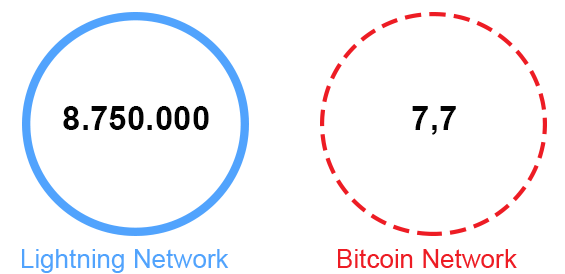
\includegraphics[scale=1.2]{images/Lightning-Network-study.png}
\captionof{figure}{Confronto tra le tecnologie Lightning network e Bitcoin: transazioni per secondo (tps)  \cite{satalight:lightningstudy}.\label{fig:velocitytx}}
\par}

\subsubsection{Timelock}

I timelock vengono introdotti nel 2016 e sono usati per esprimere restrizioni sulla modalità di spesa di UTXO al fine di consentire lo sblocco di questi ultimi solo dopo un certo evento. Questa definizione non è nuova nella tecnologia Bitcoin perché con il campo {\tt{nLockTime}} della transazione è possibile esprimere una restrizione sulla modalità di spesa di una transazione (argomento trattato nel Capitolo \ref{sec:transazioniBitcoin}); questo tipo di restrizione soffre di un problema illustrato nel seguente esempio (tratto dal libro \cite{bitcoinbook}).

\begin{example}

Supponiamo che Alice firmi una transazione spedendo uno dei suoi UTXO all'indirizzo di Bob impostando la transazione con un nLocktime proiettato nel futuro di 3 mesi.
Con questa transazione Alice e Bob sanno che:
\begin{itemize}
  \item Bob non può trasmettere la transazione per riscattare i fondi fino a quando non sono trascorsi 3 mesi.
  \item Bob può trasmettere la transazione dopo 3 mesi.
\end{itemize}
Però:
\begin{itemize}
  \item Alice può creare un'altra transazione, spendendo due volte gli stessi input senza un locktime. Pertanto, Alice può spendere lo stesso UTXO prima che siano trascorsi i 3 mesi.
  \item Bob non ha alcuna garanzia che Alice non lo farà.
\end{itemize}
\end{example}

Il concetto di timelock introduce un nuovo operatore in Bitcoin Script che prende il nome di OP\_CHECKLOCKTIMEVERIFY (CLTV); questo operatore risolve il problema illustrato nell’esempio precedente poiché blocca la  transazione a livello di script (utilizzando lo script di sblocco), ma l’operatore CLTV non punta a sostituire completamente il lavoro svolto dalla proprietà nLocktime; invece esso lavora in associazione con quest’ultima il cui valore deve essere maggiore o uguale al valore inserito nello script per rendere la transazione valida; se questa condizione viene a mancare, il sistema rifiuterà la transazione.

Sia nLockTime che CLTV sono tecniche di locking assolute in quanto specificano un quanto di tempo assoluto; con esse, quindi, non è possibile esprimere lassi di tempo relativi come, ad esempio, esprimere un lasso di tempo valido a partire dalla conferma della transazione (problema risolto dal timelock relativo, affrontato nella Sezione \ref{sec:relativetimelock}).
Un esempio di script di blocco complesso estrapolato dal \cite{bitcoinbip:bip68}:

\lstinputlisting[language=bitcoinscript, label=code:complexscript, caption=Script di Blocco che esprime una multipla condizione di spesa utilizzando OP\_CHECKLOCKTIMEVERIFY.]{code/script/examplebip68.btcs}

L’UTXO creato con il precedente script di blocco può essere sbloccato in due modi:
\begin{itemize}
  \item In qualsiasi momento  da A e B con il seguente script:
  \begin{lstlisting}[language=bitcoinscript]
   0 <A signature> <B signature> 0
  \end{lstlisting}
  \item Dopo tre mesi da A o B e C con il seguente script:
  \begin{lstlisting}[language=bitcoinscript]
   0 <A or B signature> <C signature> 1
  \end{lstlisting}
\end{itemize}

Lo script di blocco precedente esprime una condizione utilizzando l’operatore CLTV che specifica un quanto di tempo pari a tre mesi. \'E tuttavia possibile utilizzare due notazioni diverse: infatti, si può esprimere il quantitativo di tempo tramite la dichiarazione del numero di blocchi successivi oppure con un timestamp Unix. Un esempio estrapolato dal libro \cite{bitcoinbook} potrebbe essere:
\begin{itemize}
  \item Altezza attuale + 12.960 (blocchi).
  \item Timestamp corrente + 7.760.000 (secondi).
\end{itemize}

Gli script di sblocco terminano entrambi con dei suffissi, cioè 0 e 1. Questi valori servono per la corretta esecuzione della clausola if-then-else, espressa in maniera differente da una condizione if-then-else di un linguaggio moderno tipo il C++. Infatti la clausola viene definita in maniera generale in Bitcoin script come nell’esempio seguente, utilizzando il numero 0 per esprimere FALSE e 1 per TRUE.

\lstinputlisting[language=bitcoinscript, label=code:exampleifthenelse, caption=Clausola if-then-else in Bitcoin script.]{code/script/exampleIfThenElse.txt}

Bitcoin core supporta anche timelock relativi, i quali sono utili per stabilire vincoli temporali rispetto al tempo di conferma di una transazione sulla blockchain, così da permettere di esprimere un lasso di tempo relativo che dipende (in questo caso) dall’istante in cui la transazione viene confermata.
Come i timelock assoluti, i timelock relativi vengono espressi sia a livello di script che a livello di transazione; per fare ciò viene utilizzato il campo {\tt{nSequence}} all’interno della transazione di input.
Si possono distinguere attualmente due tipi di timelock relativi:

\begin{itemize}
  \item Timelock relativo bastato su consenso con nSequence.
  \item Timelock relativo basato su OP\_CHECKLOCKTIMEVERIFY(CLTV).
\end{itemize}

\subsubsection{Timelock relativo bastato su consenso con nSequence}
\label{sec:relativetimelock}
I timelock relativi possono essere impostati su ogni input di una transazione; l’introduzione in corso d’opera di questa nuova funzionalità senza produrre un hard-fork è stata resa possibile dall’esistenza del campo nSequence contenuto nella transazione di input, originariamente destinato ad una funzione (mai correttamente implementata) che consentiva la modifica della transazione durante la fase di creazione e propagazione di quest’ultima, cioè:

\begin{itemize}
  \item nSequence != 0xFFFFFFFF: La transazione poteva subire modifiche (transazione non finalizzata), quindi essa veniva mantenuta in un'area di memoria in cui tutte le transazioni pubblicate ed in attesa di essere verificate risiedono, conosciuta anche sotto il nome di {\it mempool\/}. Fin quando la transazione conteneva un valore diverso da 0xFFFFFFFF, essa non veniva presa in considerazione dai miner.
  \item nSequence = 0xFFFFFFFF: La transazione veniva considerata come “finalizzata” e quindi presa in considerazione dati miner.
\end{itemize}

Questo tipo di timelock comporta alcune modifiche alle regole di consenso, le quali in base al bit più significativo interpretano il tipo di timelock applicato (regole di consenso elencate nel \cite{bitcoinbip:bip68}).

\subsubsection{Timelock relativo basato su OP\_CHECKSEQUENCEVERIFY}

Come nel timelock assoluto, anche per il timelock relativo è stato introdotto un nuovo operatore in Bitcoin script.  Tale operatore prende il nome
OP\_CHECK\-SEQUENCE\-VERIFY (CSV) e lavora in associazione con il campo nSequence: esso verifica la distanza dal tempo in cui è stata accettata UTXO  fino al momento di valutazione dell'operatore CSV. Vediamo un esempio estrapolato dalla demo di {\it miniscript \/} illustrato nel Codice \ref{code:complexscriptnominiscritp}:

\lstinputlisting[language=bitcoinscript, label=code:complexscriptnominiscritp, caption=Uno script complesso che utilizza l’operatore OP\_CHECK\-SEQUENCE\-VERIFY.]{code/script/exampleComplexNoMiniscript.btcs}

L’esempio illustra come bloccare un input con uno script che esprime una condizione 3:3 e che solo dopo 90 giorni può essere sbloccato con una combinazione 2:3.
L’evoluzione di Bitcoin script, oltre ad aumentare i campi di applicazione di Bitcoin, aumenta drasticamente anche la difficoltà di scrittura degli script complessi che possono ora essere definiti come {\it Smart contract\/}; infatti la scrittura di Smart contract e la gestione del ciclo di vita di esso risulta essere complesso.
Per risolvere questi problema nell'agosto del 2019 è stato rilasciato il codice sorgente di un linguaggio per rappresentare Bitcoin script in modo strutturato, chiamato \emph{miniscript}.

\subsubsection{Miniscript}

Miniscript è un linguaggio implementato da Pieter Wuille, cofondatore di Blockstream e attuale sviluppatore Bitcoin core, con l'obiettivo di semplificare la scrittura di smart contract.
Miniscript è implementato in C++ ed è stato sviluppato per rappresentare un sottinsieme di Bitcoin script in modo strutturato. Ad esempio il Codice \ref{code:complexscriptnominiscritp} può essere riscritto tramite il Codice \ref{code:complexscriptminiscritp} utilizzando miniscript:

\begin{lstlisting}[language=miniscript, label={code:complexscriptminiscritp}, caption={Un esempio di utilizzo di miniscript.}]
thresh(3, pk(key_1), pk(key_2), pk(key_3), older(12960))
\end{lstlisting}

In questo esempio:
\begin{itemize}
  \item thresh(x, y, …, k): esprime un'equazione del tipo x + y + … + n = k.
  \item pk(key): effettua il controllo sulla chiave presa in input.
  \item older(k): esprime un'espressione di base per miniscript la quale effettua il controllo con il valore preso in input; nel Codice \ref{code:complexscriptminiscritp} il valore deve essere maggiore di 12960 blocchi.
\end{itemize}

\chapter{Problema}\label{chap:problema}

\section{Introduzione} \label{sec:problemaIntroduzione}

Bitcoin è a tutti gli effetti una criptovaluta pseudo-anonima. Fin dalla sua introduzione, questa  caratteristica  ha suscitato particolare interesse all’interno del \emph{Dark Web}; ciò ha reso i bitcoin, a partire dal 2011,  lo strumento di pagamento elettronico principale  per attività correlate al mercato nero di droghe, farmaci e armi, nonché uno dei principali strumenti per il riciclaggio di denaro.\\
Il concetto di distributed ledger, associato all’utilizzo estensivo di Bitcoin per attività illecite, ha dato vita a numerosi studi di analisi forense per tracciare il flusso dei bitcoin. Queste analisi vengono di solito   effettuate a partire da rapresentazioni a grafo della blockchain di Bitcoin.\\
I grafi più comunemente utilizzati sono il \emph{grafo delle transazioni} e il \emph{grafo degli address}.

\section{Grafo delle transazioni} \label{sec:grafoDelleTransazioniProblema}

Il grafo delle transazioni è un grafo diretto i cui nodi rappresentano transazioni e i cui archi denotano il consumo di transazioni da parte di altre transazioni. Come illustrato nel Capitolo \ref{chap:bitcoin}, questo grafo può essere costruito sfruttando i backlink contenuti all’interno delle transazioni di input.

\begin{example}

Consideriamo nuovamente l’Esempio \ref{example:aliceBobFirst}, nel quale Alice vuole trasferire 0.00700767 bitcoin a Bob. Esaminando la nuova  transazione prodotta da Alice e indirizzata a Bob con l’id \say{ddd587d\-54b693\-a9bc9bda\-2218c6f5e17\-979f6ac53755\-c5c1f668f3fa\-728e472d}, possiamo osservare che all’interno della transazione di input era contenuto un id di transazione appartenente ad un precendete UTXO in possesso di Alice (\say{a57c2a4\-27dfa\-591b1243\-343c8413\-c249faac\-3e5df2fe\-4fa1fc93dca\-3d904f3c7}). Conseguentemente, il frammento di grafo corrispondente a questo scambio di bitcoin, mostrato in Figura \ref{fig:graphtxproblem}, contiene due nodi, il primo dei quali corrisponde all'UTXO di Alice, mentre il secondo alla transazione di Alice verso Bob.

\begin{figure}
\centering
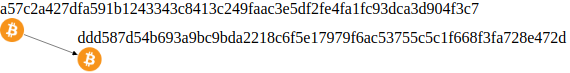
\includegraphics[scale=0.35]{images/exampleWithGraph/aliceBoxTx.png}
\caption{Frammento del grafo delle transazioni relativo alla  transazione tra Alice e Bob descritta nell’Esempio \ref{example:aliceBobFirst}.\label{fig:graphtxproblem}}
\end{figure}

\end{example}

\section{Grafo degli address} \label{sec:grafoDegliAddressProblema}

Il grafo degli address è un grafo diretto i cui nodi sono address e i cui archi rappresentano flussi di bitcoin da un address ad un altro, indotti direttamente o indirettamente da transazioni Bitcoin.

La creazione di questa tipologia di grafi è molto meno intuitiva, poiché, come visto nel Capitolo \ref{chap:bitcoin}, le transazioni non contengono alcun riferimento esplicito a wallet o persone, sfruttando, invece, chiavi private e corrispondenti chiavi pubbliche. Gli address generati attraverso la chiave pubblica sono contenuti all’interno dello script di blocco in modo da rendere la transazione sbloccabile solo dal proprietario dell’address. \\
Come descritto nella Sezione \ref{sec:bitcoinScriptBitcoin}, gli address possono essere originati anche da uno script tipo P2SH, P2WPKH e P2WSH; ciò rende la creazione del grafo degli address molto insidiosa, perché gli address ricavati dagli script (se utilizzati correttamente) sono univoci e quindi rappresenterebbero un’identità diversa all’interno del grafo, anche se molti di questi potrebbero appartenere in realtà allo stesso wallet.

\begin{example}
Consideriamo nuovamente l’Esempio \ref{example:aliceBobFirst}. In tale esempio  Alice genera una nuova transazione consumando un suo UTXO con un valore maggiore o uguale alla quantità  di bitcoin che desidera trasferire; nell'esempio viene utilizzato un UTXO con un quantitativo maggiore, il che comporta così la generazione di una exchange transaction per riaccreditare la somma eccedente attraverso un nuovo UTXO.

Modellare questo semplice trasferimento può portare a due probelamtiche.

\begin{itemize}
  \item L’exchange transaction potrebbe contenere un address differente: in questo specifico caso la transazione contiene un address ricavato da uno script Witness (che potrebbe essere ricavato dalla medesima chiave pubblica o da chiavi pubbliche distinte contenute all’interno del wallet).

  \item L'exchange transaction potrebbe contenere uno script P2PKH e quindi un indirizzo primitivo, ma quest’ultimo potrebbe essere differente dall’address di origine. Questo lascerebbe pensare che i bitcoin  siano diretti verso un nuovo proprietario, mentre nella maggior parte dei casi è solo una tecnica per aumentare la privacy utilizzata dagli wallet.
Infatti, molti  wallet comunemente utilizzati contengono un set di chiavi private che permette loro di generare un address diverso ad ogni nuova operazione.
\end{itemize}

\end{example}

La creazione del grafo degli address comporta quindi una serie di problematiche riguardanti gli address, che possono rivelarsi molto significative.

\paragraph*{Indirizzi originati da script}  Il destinatario potrebbe usare indirizzi originati da script (come un address P2SH) rendendo così difficile associare l’appartenenza allo stesso wallet di più address; in alternativa,  l’address potrebbe camuffare uno script P2MS N:M con destinatari distinti. \\
  In Figura \ref{fig:alicebobgraphaddress} viene rappresentato il grafo di address coinvolti nell’Esempio \ref{example:aliceBobFirst}, dove l’address \say{33mMAc6nGyENdKMQTr5SrKoEkwNTeZQUx9} rappresenta una particolare tipologia di indirizzo utilizzato da Bob; infatti l’address viene ricavato da uno script P2WSH che a sua volta camuffa uno script P2MS. \\
  Bob ha infatti utilizzato uno script P2MS con due address differenti al suo interno, appartenenti allo stesso wallet. \\
  Gli address che iniziano per \say{bc1q} appartengono al medesimo wallet di Alice; i nodi corrispondenti sono collegati attraverso un arco corrispondente ad una exchange transaction.

\begin{figure}
\centering
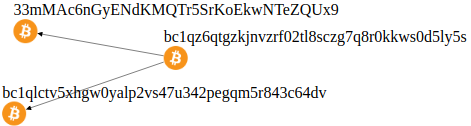
\includegraphics[scale=0.43]{images/exampleWithGraph/exchange-transaction-alice-bob.png}
  \caption{Frammento del grafo di address corrispondente alla transazione illustrata nell’Esempio \ref{example:aliceBobFirst}.\label{fig:alicebobgraphaddress}}
\end{figure}

\paragraph*{Address ricavati da chiavi pubbliche diverse} La generazione delle exchange transaction contiene, nella maggior parte dei casi, un address ricavato da una chiave pubblica diversa, appartenente allo stesso wallet, come illustrato nel seguente esempio.

\begin{example} \label{example:newalicebobaddress}
   Si consideri un nuovo scenario dove Alice spedisce dei bitcoin a Bob ed entrambi i partecipanti utilizzano address primitivi:  Alice invia all’indirizzo di Bob 0.00336527 bitcoin, generando una nuova transazione con il seguente id \say{8b22a9\-d19ee58ee1b\-5283632f70\-fbeceaf13\-948dbc3d\-48ea22c02\-1a1d82\-e1f06} verso l’address di Bob \say{1CP\-D7Dqgu\-ruujwvfa\-egKsV6ew\-iFvSZTiB3}.
    Il wallet di Alice utilizza un suo UTXO per per effettuare la spedizione di bitcoin con un valore maggiore del necessario, quindi il wallet è costretto a generare una exchange transaction per dividere UTXO. \\
    L’UTXO di Alice con un valore di bitcoin pari a 0.00682055 bitcoin si frammenta in due nuove transazioni:

    \begin{itemize}
      \item La transazione verso Bob del valore di 0.00336527 bitcoin.
      \item L’exchange transaction verso il wallet di Alice del valore di 0.00341851 bitcoin.
    \end{itemize}

La Figura \ref{fig:newalicebobaddress} rappresenta il grafo risultante degli address coinvolti.

\begin{figure}
\centering
    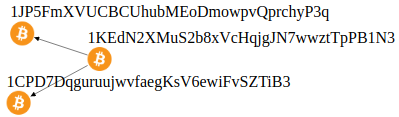
\includegraphics[scale=0.43]{images/exampleWithGraph/example-p2pkh-exchange-transaction.png}
    \caption{Frammento  del grafo degli address coinvolti nella transazione dell’esempio \ref{example:newalicebobaddress}.\label{fig:newalicebobaddress}}
\end{figure}

    In Figura \ref{fig:newalicebobaddress} si possono osservare tre address distinti originati da chiavi pubbliche distinte, dove però i proprietari sono solo Alice e Bob:
    \begin{itemize}
      \item Gli address di Alice sono:
      \begin{enumerate}
      \item \say{1KE\-dN2XMu\-S2b8xVc\-HqjgJN\-7wwztT\-pPB1N3}, che rappresenta l’address di orgine;

      \item \say{1JP5F\-mXVUCB\-CUhubME\-oDmowpv\-Qprchy\-P3q} che rappresenta l’address a cui viene indirizzata l’exchange transaction. Entrambi gli address appartengono al wallet di Alice, ma sono originati da chiavi pubbliche diverse.
      \end{enumerate}
      \item L’address di Bob inviato ad Alice per eseguire la spedizione di Bitcoin: \say{1CPD7Dq\-guruujwvf\-aegKsV6ew\-iFvSZTiB3}.
    \end{itemize}
  \end{example}

Nelle prime versioni di Bitcoin, non tutti i wallet contenevano un set di chiavi private e questo comportava la creazione di exchange transaction verso il medesimo address, come mostrato nell'esempio \ref{ex:sameaddr}.

\begin{example}\label{ex:sameaddr}

  Prendiamo in esame la transazione con il seguente id \say{15bf\-8b35c\-9210efe7e448\-c5fc6b69b47b3a8\-cac9c148c7cc\-57c65f266\-384d9b8} in cui possiamo osservare la presenza dell’address \say{1EinmJDn\-33yFPGafKu\-Cw2guUqPSMaNKo5v} sia in output che in input.
  La Figura \ref{fig:exchangeaddressrecicle} rappresenta la transazione ricercata attraverso un esploratore blockchain.

\begin{figure}
\centering
  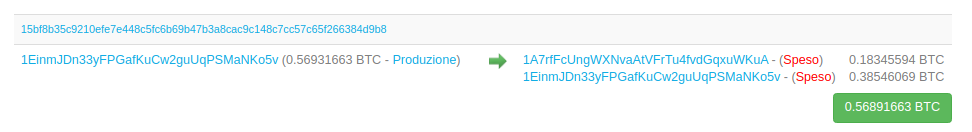
\includegraphics[scale=0.35]{images/exampleWithGraph/exchange-tx-with-same-address.png}
  \caption{Una exchange transaction verso lo stesso indirizzo di origine\cite{blockstream:esplora}.\label{fig:exchangeaddressrecicle}}
\end{figure}

  In questo caso il flusso di bitcoin è chiaro e il corrispondente grafo degli address è mostrato  nella Figura \ref{fig:graphAddresssameaddresschange}.

\begin{figure}
\centering
  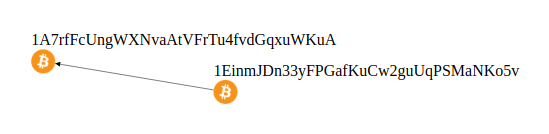
\includegraphics[scale=0.48]{images/exampleWithGraph/exchange-tx-with-same-address-graph.png}
  \caption{Il grafo degli address coinvolti nella transazione con id 15bf8\-b35c9210\-efe7e448c5fc\-6b69b47b3a\-8cac9c14\-8c7cc57c6\-5f26638\-4d9b8.\label{fig:graphAddresssameaddresschange}}
\end{figure}
\end{example}

La costruzione del grafo degli address, oltre ad essere insidiosa per i problemi relativi alla frammentazione degli address, costringe ad accedere alle transazioni di output contenute all’interno delle transazioni, il cui riferimento risiede nelle transazioni di input della nuova transazione, per prelevare l’address di origine.
La Figura \ref{fig:processgetorigin} illustra il procedimento per ottenere l’address di origine dell’Esempio \ref{example:aliceBobFirst}.

{\vspace{15pt}
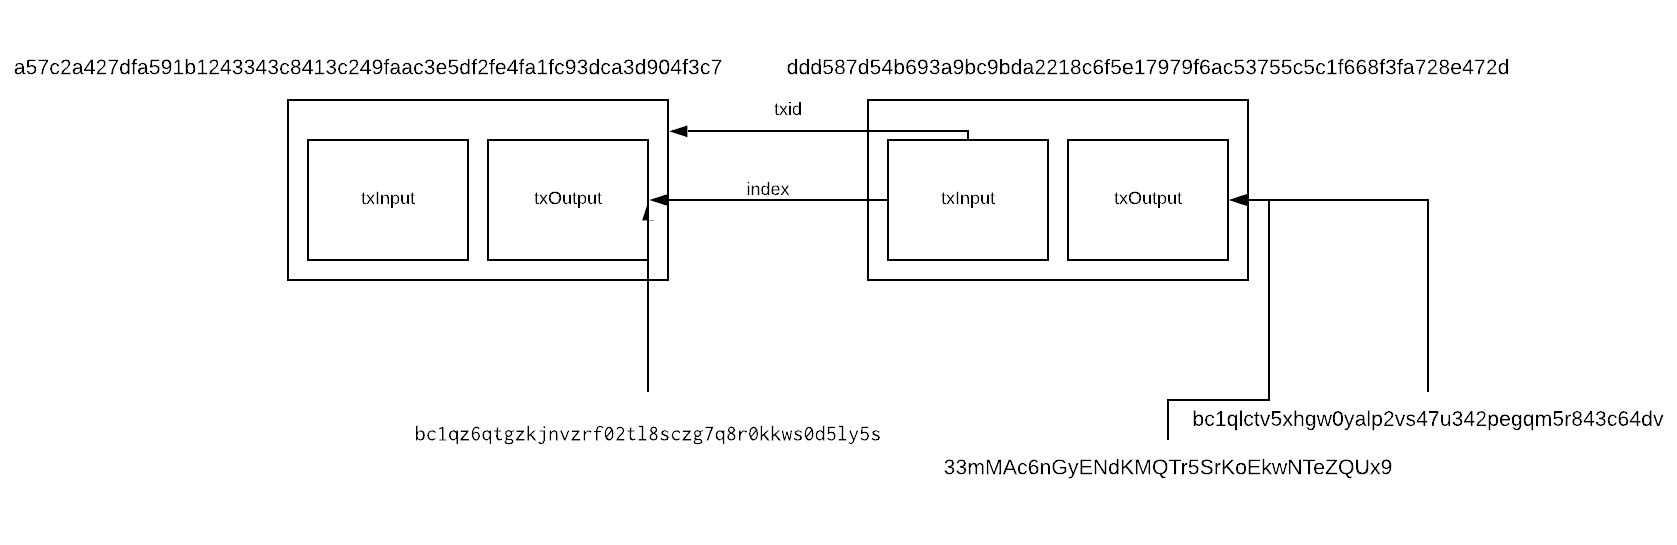
\includegraphics[scale=0.25]{images/howFindTheAddressTo.png}
\captionof{figure}{Rappresentazione del procedimento per determinare l’address di origine.\label{fig:processgetorigin}}
\vspace{10pt}
\par}

\chapter{Stato dell'Arte}\label{chap:riferimentiStrotici}

%\section{Introduzione} \label{sec:riferimentiStorici}
%Cosa posso inserire?

\section{BlockSci} \label{sec:riferimentiStorici}

BlockSci \cite{blocksci:article} è un sistema open source, scritto in C++, per l'analisi di blockchain basate sull'organizzazione dati di Bitcoin. Sviluppato dall'Università di Princeton, BlockSci estrae i dati dalla blockchain di BitCoin attraverso l'utilizzo del framework RPC di BitCoin e di un parser per l'analisi delle informazioni serializzate dal nodo Bitcoin; i dati estratti vengono salvati in flat-file e interrogati attraverso SQLite.
BlockSci, inoltre, offre un sofisticato sistema per l'analisi dei dati estratti con cui si ha la possibilità di implementare e applicare algoritmi di analisi sulla rete Bitcoin.

In questa sezione ci concentreremo  solo sul modulo relativo al parser e sull'organizzazione delle informazioni estratte. Il parser di BlockSci legge le informazioni della blockchain sequenzialmente e, durante la lettura, applica  una serie di ottimizzazioni per il corretto funzionamento del modulo di analisi.
Il risultato della scansione sequenziale dei blocchi è un grafo delle transazioni minimale; il grafo è memorizzato in una singola tabella sequenziale, le cui entry hanno il formato mostrato in Tabella \ref{tab:blockSciSerialization}.

\begin{table}
       \centering\small
           \begin{tabular}{|c|c|}
               \hline
                 \multicolumn{2}{|c|}{\textbf{Transaction}} \\
                 %\cmidrule(lr){1-2}
                 \hline
                 \multicolumn{1}{|c|}{Size} & \multicolumn{1}{c|}{Description} \\
               \hline \hline
               32 bit & Size   \\
               \hline
               32 bit & LockTime \\
               \hline
               16 bit & Input count \\
               \hline
               16 bit & Output count \\
               \hline
               128 bits each & Outputs \\
               \hline
               128 bits each & Inputs \\
               \hline
       \end{tabular}
       \caption{Struttura delle transazioni in BlockSci per la costruzione del grafo delle transazioni \cite{blocksci:article}.\label{tab:blockSciSerialization}}
   \end{table}

In  \cite{blocksci:article} Kalodner et al. descrivono i risultati di alcuni test relativi all'efficienza del parser; in tali test, il parser ha impiegato all'incirca 11 ore per effettuare l'estrazione dei dati dalla blockchain di Bitcoin\footnote{Tali risultati fanno riferimento alla dimensione della blockchain assunta nell'agosto del 2017: 478,559 blocchi e 140 GB di spazio totale.}; aumentando la dimensione della memeoria allocata a BlockSci si possono ottenere prestazioni migliori.

\section{BiVA} \label{sec:biva}

BiVA (Bitcoin Network Visualization \& Analysis) è un software sviluppato dall'Università di Singapore che utilizza Neo4J \cite{neo4j} per la costruzione di un grafo di address attraverso l'estrapolazione dei dati tramite il framework RPC di Bitcoin-core; esso, inoltre, implementa un algoritmo di analisi su grafo per la ricerca degli address più utilizzati all'interno della blockchain di Bitcoin.\\
In \cite{DBLP:conf/icdm/OggierPD18} Oggier et al. descrivono prevalentemente l'algoritmo di analisi utilizzato e non riportano dettagli sull'implementazione né risultati sperimentali relativi all'estrazione dei dati; tuttavia, poiché il framework RPC non è progettato  per l'estrazione completa dei dati dalla blockchain, le tempistiche dovrebbero essere abbastanza elevate utilizzando un software \emph{single thread}.\\
Una porzione di grafo prodotto attraverso BiVA è rappresentata in Figura \ref{fig:bivaGraph}.

\begin{figure}
\centering
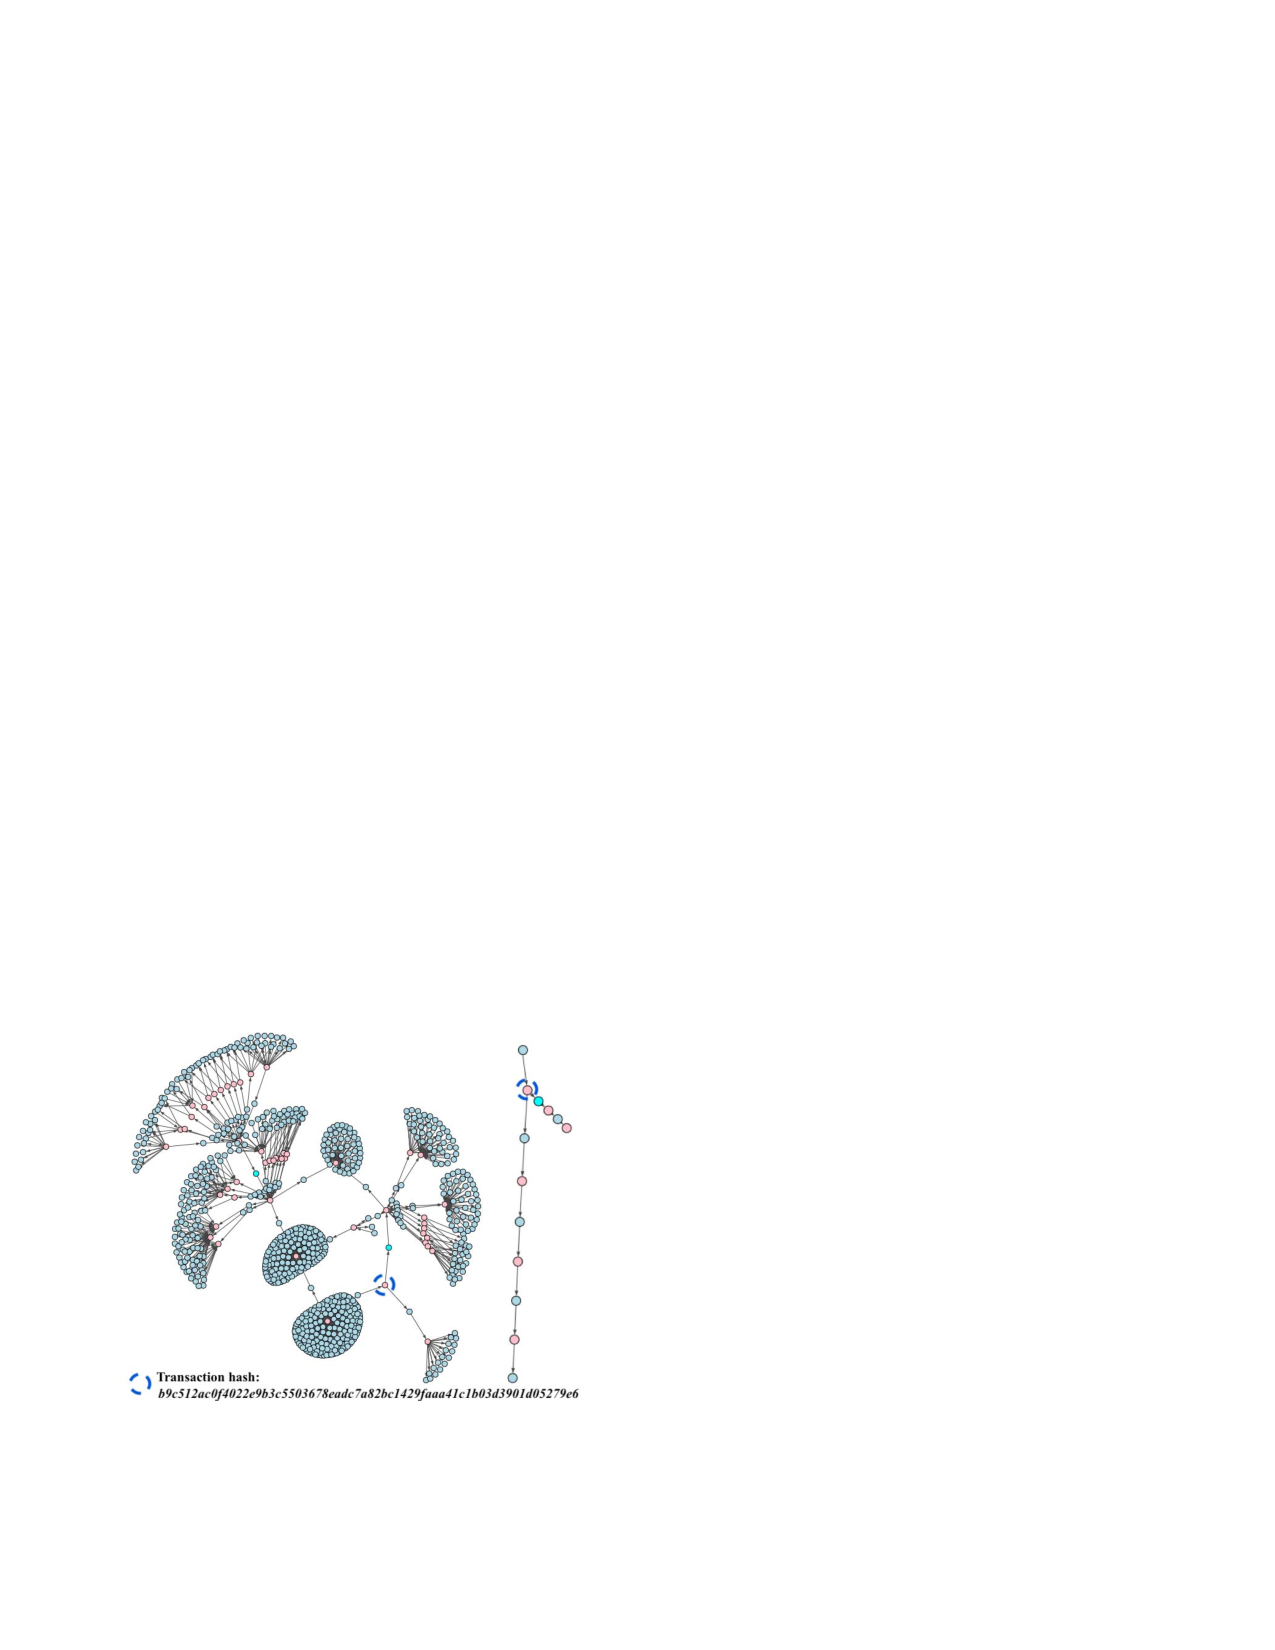
\includegraphics[scale=1.0]{images/bivaGraph.pdf}
\caption{Frammento del grafo degli address creato attraverso BiVA \cite{DBLP:conf/icdm/OggierPD18}.\label{fig:bivaGraph}}
\end{figure}


\section{Bitcoin Transaction Visualization} \label{sec:bitcoinTransactionVis}

Uno studio condotto dall'Universita di Saskatchewan e pubblicato nel articolo \cite{BitcoinBlockchainTransactionsVisualization:article} descrive la creazione di un grafo di transazioni localizzato attraverso l'utilizzo delle API di \url{https://blockchain.com}.\\
L'utilizzo di queste API ha permesso di localizzare le transazioni attraverso la sua posizione geografica grazie all'IP messo a disposione della servizio per ogni transazione (quando questo ip è esposto).\\
La demo per la dimostrazione di questo studio viene sviluppata attraverso tecnologie web con un uso estensivo di JQuery, La Figura \ref{fig:bitcoinTransactionVis} ne rappresenta un esempio.

\begin{figure}[H]
\centering
\includegraphics[scale=0.1]{images/vs_article.pdf}
\caption{Frammento del grafo di transazioni prodotto attraverso la demo pubblicata nell'articolo \cite{BitcoinBlockchainTransactionsVisualization:article}.\label{fig:bitcoinTransactionVis}}
\end{figure}

\chapter{Tecnologie Utilizzate}\label{chap:tecnologieUtilizzate}

\section{Bitcoin-Cryptography-Library} \label{sec:cryptographyBitcoinLib}

La libreria Bitcoin-Cryptography-Library \cite{Bitcoin-Cryptography-Library:github} ha permesso di importare la crittografia di base utilizzata in Bitcoin. Tale  libreria è stata sviluppata in C++11 e in Java dallo sviluppatore Nayuki; la libreria risiede su Github sotto licenza MIT ed è progettata principalmente per microcontrollori ad 8 bit (e.g., Arduino, Atmel megaAVR/ATmega, ecc) con il supporto anche per dispositivi con architetture x86, x86-64 e 32-bit ARM.

\section{RapidJSON} \label{sec:rapidjsonLib}

La libreria RapidJSON \cite{rapidjson:github} ha permesso la decodifica in formato serializzato delle informazioni lette dal parser consentendo di creare una versione JSON della blockchain; è scritta in C++ dal team di sviluppo Tencent ed è rilasciata su Github sotto licenza BSD.
Con l’utilizzo della libreria siamo riusciti ad introdurre all’interno del parser una deserializzazione quasi \emph{real-time} di ogni blocco.


\section{Bitcoin-api-cpp} \label{sec:bitcoinApiLib}

La libreria bitcoin-api-cpp \cite{bitcoin-api-cpp:github} implementa un wrapper per il framework RPC di Bitcoin-core; tale libreria risiede su Github sotto licenza MIT ed è stata  implementata in C++ dallo sviluppatore Krzysztof Okupski.
Con l'utilizzo di questa liberia siamo riusciti ad'interfacciarci con il nodo Bitcoin per deserializzare le informazioni relative allo script di blocco.

\section{JSON-RPC 1.0} \label{sec:jsonrpchttp}

Bitcoin-core offre un framework RPC (Remote Procedure Call) basato sul protocollo HTTP per consentire l'utilizzo dei servizi offerti dal nodo Bitcoin, quali, ad esempio,  esaminare lo stato della blockchain oppure effettuare la crezione di transazioni in formato esadecimale.

Abbiamo utilizzato questo servizio offerto da Bitcoin-core per l'estrazione dell'address dallo script di blocco; esso, inoltre ci ha consentito di ricavare i dati della transazionie precedente contenuta all'interno della transazione di input attualmente esaminata senza l'implementazione di una cache, a scapito, tuttavia, dell'efficienza della soluzione proposta.

\section{Zlib} \label{sec:zlib}

La libreria Zlib \cite{zlib:github} è una famosa libreria di compressione open source, sviluppata da Jean-loup Gailly e Mark Adler in C; essa è divenuta  uno standard RFC nel maggio 1996 ed è stata inserita all'interno del Java Development Kit a partire dalla versione 1.1.
La libreria viene utilizzata per ridurre lo spazio richiesto dalle informazioni prodotte riguardanti i grafi.

\section{Bitcoin core library} \label{sec:bitcoinCoreLib}

Sono state utilizzate alcune parti del codice sorgente di Bitcoin core per diminuire il quantitativo di test da produrre e sopratutto diminuire il numero di errori possibili durante il parsing dei dati.\\
Le librerie estratte sono:
\begin{itemize}
  \item La libreria \say{serialize.h} con le relative dipendenze, con cui è stato possibile serializzare/deserializzare ogni singolo tipo di dato nel formato corretto, ad esempio: le informazioni vengono deserializzate in \emph{little andian} e solo alcuni tipi di dato, come gli hash, vengono deserializzati in \emph{big endian}.
  \item La libreria \say{endian.h} con le relative dipendenze, con cui è stato possibile gestire rappresentazione dei dati in formato little endian e big endian.
  \item La libreria \say{uint256.h} con le relative dipendenze, con cui è stato implementato il tipo di dato per rappresentare gli hash.
\end{itemize}
Tutte le librerie utilizzate ed estratte da Bitcoin core sono rilasciate sotto licenza MIT.

\chapter{Soluzione Proposta}\label{chap:soluzioneproposta}

\section{Introduzione} \label{sec:solIntroduction}

L'estrazione dei dati dalla blockchain di Bitcoin ha richiesto un analisi preliminare della tecnologia ed in particolare sul modo in cui vengono serializzati i dati dal client; questa prima analisi ha permesso di osservare la rapida crescita dello spazio richiesto della blockchain, rappresentata dalla Figura \ref{fig:dimensionBlockchain}.

{\vspace{15pt}
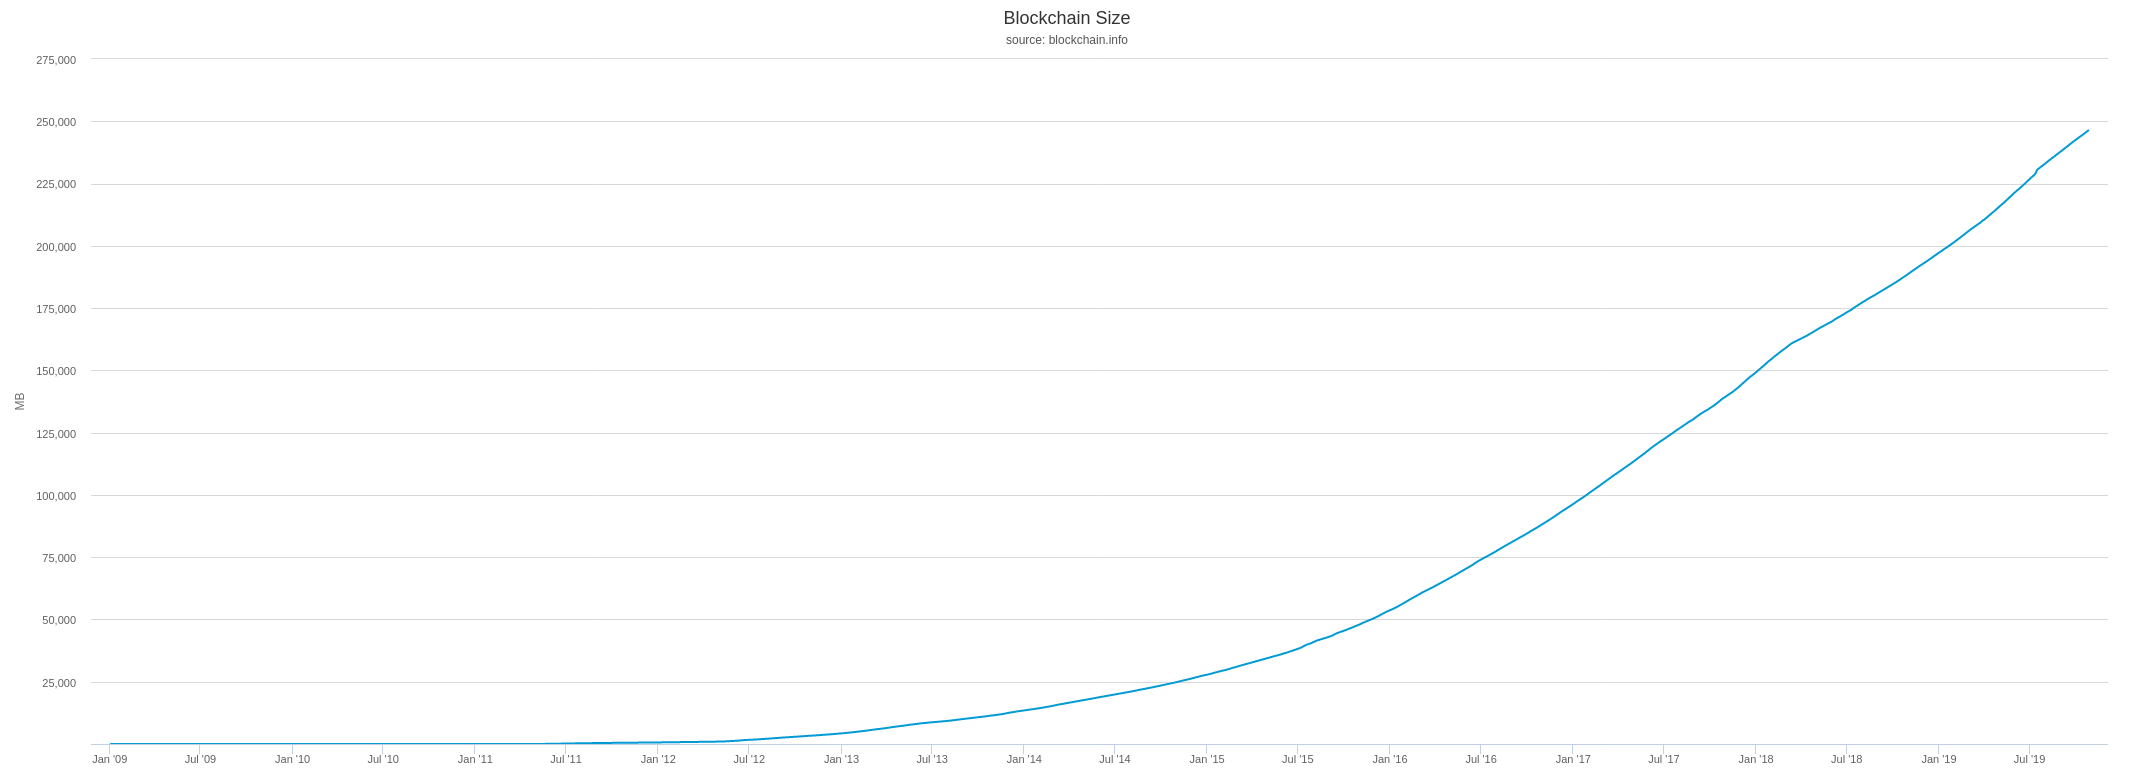
\includegraphics[scale=0.18]{images/blockchain-size.png}
\captionof{figure}{Crescita della dimenzione della blockchain di Bitcoin nel tempo.\label{fig:dimensionBlockchain}}
\vspace{10pt}
\par}

La rapida crescita della blockchain porta alle seguenti problematiche:

\begin{itemize}
  \item L'estrazione dei dati dalla blockchain di Bitcoin richiede un software scalabile per permettere in qualsiasi condizione di utilizzo l'estrazione dei dati.
  \item L'organizzazione dei dati estratti della blockchain deve essere versatile per consentire analisi differenti, in modo tale da non richiedere una seconda scansione a seconda del tipo di analisi da effettuare.
\end{itemize}

\section{SpyCBlock} \label{sec:spycblock}

SpyCBlock rappresenta la soluzione proposta per l'estrazione di dati dalla blockchain di Bitcoin in modo scalabile. Attraverso SpyCBlock viene effettua la creazione dei due principali grafi per l'analisi forense; SpyCBlock, inoltre, produce in formato JSON (JavaScript Object Notation) una deserializzazione completa della blockchain, arricchita con informazioni addizionali; infatti, come descritto nel Capitolo \ref{chap:bitcoin}, i blocchi e le transazioni contengono solo gli identificativi dei loro predecessori, il che costringe il parser in fase di deserializzazione a ricostruire l'hash della transazione e del rispettivo blocco preso in analisi; questo è stato reso possibile dalla libreria \say{Bitcoin-Cryptography-Library} descritta nel Capitolo \ref{sec:cryptographyBitcoinLib}.\\
SpyCBlock rappresenta un prototipo di un software di analisi accademico, sviluppato interamente in C++14 e risiede su Github sotto licenza Apache License 2.0. Esso è l'implementazione di un parser delle informazioni serializzate dal nodo Bitcoin e utilizza le librerie di Bitcoin-core, descritte nella Sezione \ref{sec:bitcoinCoreLib}.\\
Il software è stato implementato utilizzando una metodologia agile; infatti lo sviluppo di SpyCBlock e lo studio della tecnologia Bitcoin sono avvenute in parallelo. Questo ha permesso di convalidare tutte le nozioni studiate sulla tecnologia, basando l'intero ciclo di sviluppo sulla produzione di test di unità (9 batterie di test, per un totale di 46 test di unità).\\
I dati decodificati del singolo blocco vengono verificati all'interno dei test di unità utilizzando dati prototti attraverso l'utilizzo di altri parser, come Blocktools \cite{parser:blocktools}, e attraverso i dati esposti dagli explorer, come Explora \cite{blockstream:esplora} e Blockchain explorer\cite{blockchain:explorer}.\\
Inoltre il parser è costituito da un sottomodulo per consentire la costruzione del grafo di address, utilizzando il nodo Bitcoin-core per effettuare la decodifica degli script.

\section{SpyCBlockRPC} \label{sec:spycblockrpc}

SpyCBlockRPC è un sottomodulo di SpyCBlock descritto nella Sezione \ref{sec:spycblock}; esso viene sviluppato in C++11 e risiede su Github sotto licenza Apache License 2.0.\\
SpyCBlockRPC rappresenta l'implementazione di un wrapper della libreria bitcoin-api-cpp descritta nella Sezione \ref{sec:bitcoinApiLib} che consente di effettuare interi casi d'uso costituiti da più comandi RPC di Bitcoin-core.
L'utilizzo di questo sottomodulo permette al parser di rimanere disaccoppiato dalla libreria bitcoin-cpp-api e dal framework RPC; inoltre il sottomodulo fornisce un'interfaccia comune per la serializzazione di qualsiasi tipo di grafo che si voglia costruire usando le informazioni della blockchain.\\
SpyCBlock utilizza l'interfaccia comune offerta da SpyCBlockRPC per implementare la serializzazione del grafo di transazioni ed inoltre utilizza l'implementazione offerta dal sottomodulo SpyCBlockRPC per serializzare il grafo degli address.

\section{Serializzazione della blockchain in formato JSON} \label{sec:spycblock}

Prima di effettuare la creazione dei grafi, descritti nelle sezioni successive, abbiamo dovuto affrontare varie problematiche che si sono presentate durante la fase di decodifica delle informazioni. Infatti, l'aggiornamento al Segregated Witness (descritto nella Sezione \ref{sec:transazionibitcoincore}) ha introdotto alcune modifiche anche nel modo in cui viene serializzata una transazione; questo costringe il parser a utilizzare, a seconda del tipo di transazione, metodi diversi di deserializzazione.
L'aggiornamento al Segregated Witness ha introdutto tre nuove informazioni all'interno delle transazioni, che sono:
\begin{itemize}
  \item La proprietà flag.
  \item La proprietà Marker.
  \item Se le due propietà precedenti sono rispettivamente 0 e 1, allora all'interno della transazione esisterà una lista di Script Witness, descritti nella Sezione \ref{sec:transazionibitcoincore}, che vengono denominati \say{TransactionWitness}.
\end{itemize}

Il Frammento di codice descritto nell'Appendice \ref{sec:decodeTransactionCode} rappresenta il codice con cui è possibile deserializzare una transazione dopo l'aggiornamento al Segregated Witness (viene usato Python per brevità).\\
I problemi relativi alla deserializzazione dei dati, combinati con la grande quantità di dati da deserializzare\footnote{In data {\today} la dimensione della blockchain di Bitcoin è pari a 270 Gb.}, hanno richiesto la progettazione di un metodo di testing automatico sull'intera blockchain oppure su un parte specifica.
Questo ha richiesto di convertire le informazioni deserializzate dal parser in un formato universale per eseguire l'elaborazione di queste informazioni con qualsiasi linguaggio.\\
Il formato file utilizzato per la codifica delle informazioni è il formato JSON (JavaScript Object Notation) e la libreria RapidJSON descritta nella Sezione \ref{sec:rapidjsonLib} ha reso possibile la serializzazione delle informazioni lette dal parser in maniera streaming: ogni blocco decodificato viene serializzato in JSON immediatamente con la conseguenza di un utilizzo di memoria RAM irrisorio.\\
L'adozione del formato JSON per l'organizzazione dei dati ha portato i seguenti benefici:
\begin{itemize}
  \item I dati serializzati in JSON possono essere testati in maniera automatizzata attraverso l'uso di API esterne oppure attraverso il framework RPC di Bitcoin-core descritto nella Sezione \ref{sec:jsonrpchttp}.
  \item I dati serializzati in JSON possono essere testati a vari livelli di precisone. A titolo di esempio, un eventuale errore di deserializzazione in un determinato punto della blockchain può essere individuato facilmente e osservato attraverso il suo corrispettivo in formato JSON.
  Questo evita l'uso del debugger per errori introdotti in fase di sviluppo dal programmatore, perché essi sono facilmente individuabili se i dati sono convertiti in un formato comprensibile per l'uomo.
  \item La rappresentazione JSON dell'intera blockchain offre anche la possibilità di eseguire ulteriori tipi di analisi all'interno della blockchain di Bitcoin; ad esempio attraverso l'utilizzo di una sempice applicazione di analisi descritta nella Sezione \ref{sec:solDemo}, è possibile sfruttare i dati in formato JSON per un analisi sui tipi di script utilizzati all'interno della blockchain.
  In Figura \ref{fig:chartOPRETURN} viene riportato un grafico che rappresenta l'utilizzo estensivo dell'operatore OP\_RETURN (descritto nella Sezione \ref{sub:sectionNUllaDataScript}) e quindi l'utilizzo della blockchain di Bitcoin per l'archiviazione di dati.
\end{itemize}

{\centering
\vspace{15pt}
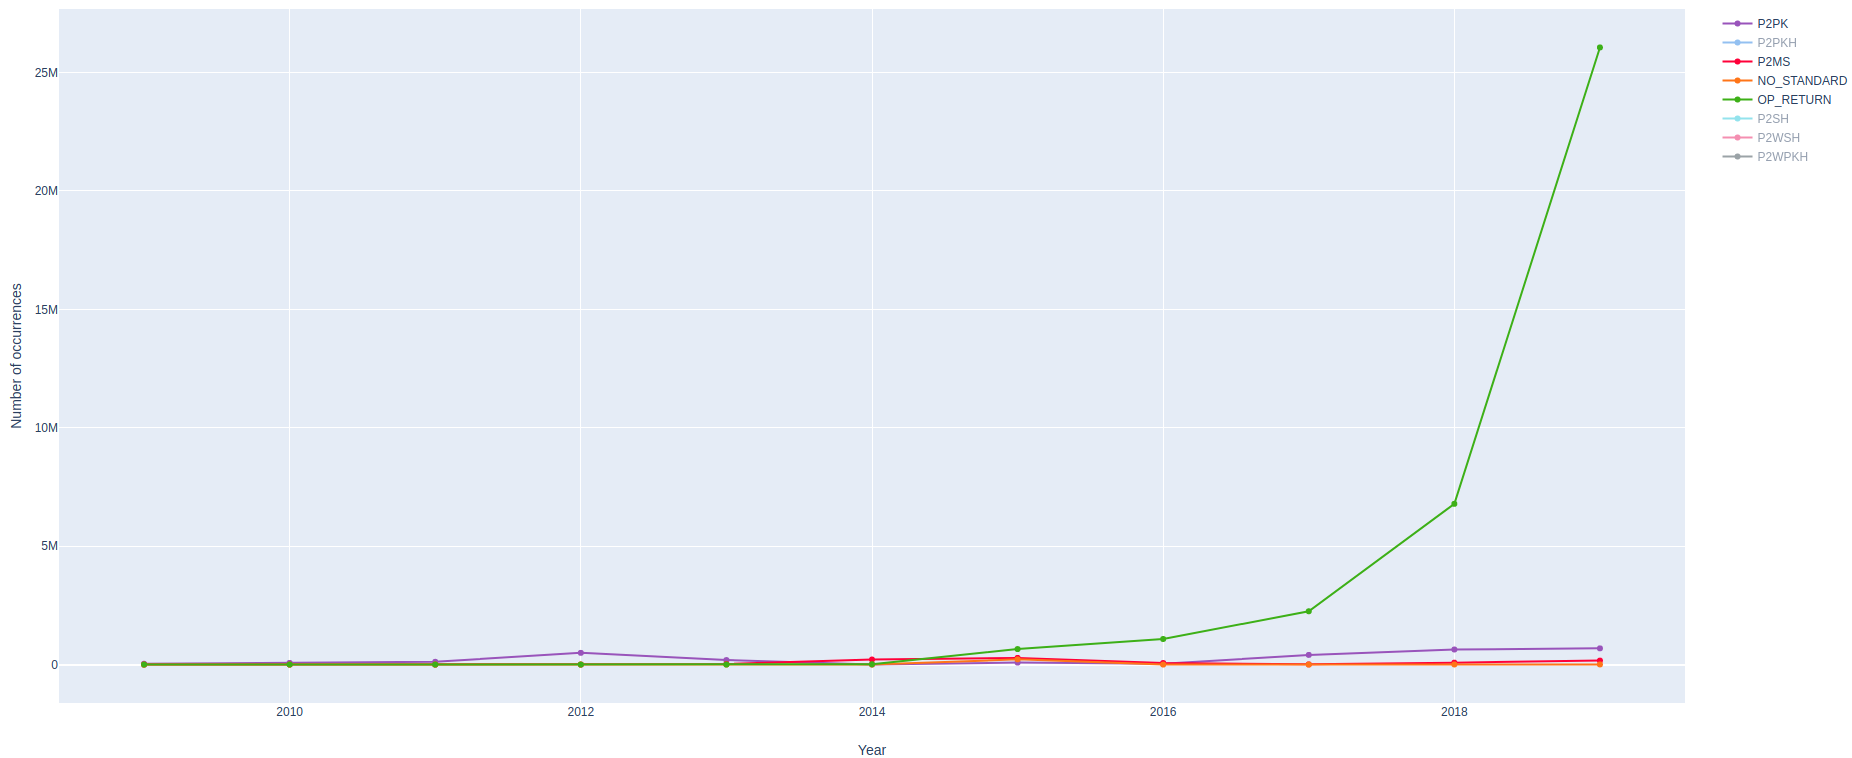
\includegraphics[scale=0.5]{images/OP_RETUTN_chart.png}
\captionof{figure}{Frammento di grafico estrapolato dall'applicazione della Sezione \ref{sec:AnalyticsPyBlock} dove viene rappresentato l'utilizzo del operatore OP\_RETURN all'interno degli script di blocco.\label{fig:chartOPRETURN}}
\vspace{10pt}
\par}


\section{Grafo delle transazioni} \label{sec:solGraphTX}

Dopo un accurata convalida dei dati deserializzati dal parser, abbiamo eseguito una nuova iterazione all'interno del ciclo di sviluppo del software, aggiungendo all'interno del parser la possibilità di serializzare i dati letti come nodi e archi di un grafo orientato.\\
Ogni transazione, infatti, genera un arco $(u, v)$ in cui il nodo di origine $u$ rappresenta l'hash della transazione attualmente analizzata e il nodo di arrivo $v$ rappresenta l'hash della transazione precedente, contenuta all'interno del tipo di dato \say{Outpoint} nella transazione di input (illustrato nella Sezione \ref{sec:transazionibitcoincore}).\\
Come descritto nella Sezione \ref{sec:grafoDelleTransazioniProblema}, la creazione del grafo delle transazioni risulta abbastanza intuitiva, ma la struttura dati della blockchain di Bitcoin costringe il parser al calcolo dell'hash della transazione attualmente analizzata perché esso non viene incluso; per fare questo il parser riconverte in memoria i dati nel formato di serializzazione originario.
In seguito alla riconversione con l'utilizzo della libreria Bitcoin-Cryptography-Library descritta nella Sezione \ref{sec:cryptographyBitcoinLib}, viene eseguito il doppio SHA256 dei bit riguardanti le informazioni in formato esadecimale, in cui ogni tipo della struttura viene prima convertito nel formato little-endian.\\

\begin{example}

Prendiamo in considerazione la transazione coinbase del blocco di genesi\footnote{Il blocco di genesi è anche conosciuto come blocco 0 oppure blocco \emph{never mined}, i cui dati sono stati codificati da Satoshi Nakamoto all'interno del codice sorgente di Bitcoin-core. Introdurre dei nuovi dati all'interno del blocco di genesi implica la creazione di una nuova blockchain.} rappresentata nella Figura \ref{fig:txGenesisBlock}.

{\centering
\vspace{15pt}
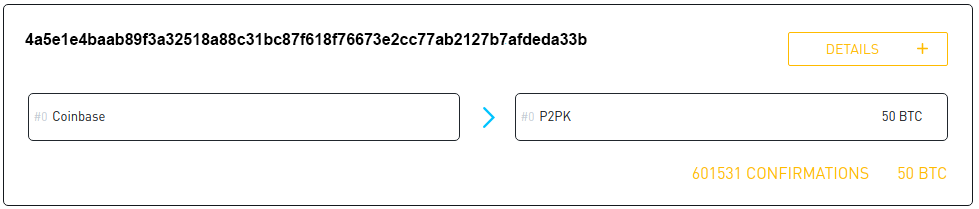
\includegraphics[scale=0.35]{images/coinbase_tx_genesis_block.png}
\captionof{figure}{Rappresentazione attraverso un'explorer \cite{blockstream:esplora} della transazione coinbase contenuta all'interno del blocco di genesi.\label{fig:txGenesisBlock}}
\vspace{10pt}
\par}

Analizzando i dati estratti dal parser possiamo notare che gli explorer non mostrano molte delle informazioni contenute all'interno delle transazioni; utilizzando invece il frammento di serializzazione JSON descritto nell'Appendice \ref{sec:genesiBlockTxJSON} in cui viene raffigurata la prima transazione nella blockchain di Bitcoin, possiamo notare tutte le informazioni realmente contenute nella struttara di una transazione.
Per effettuare il calcolo dell'hash della transazione il parser riconverte ogni tipo di dato nel formato little-endian e infine converte il valore nel corrispettivo esadecimale. La porzione di Codice \ref{code:typehexTxCpp} riporta il valore convertito con il processo descritto in predecenza.

\lstinputlisting[language=C++, label=code:typehexTxCpp, caption=Frammento di codice che rappresenta il valore esadecimale di ogni dipo di dato della transazione.]{code/coinBaseTxGenesisBlockHex.cpp}

Infine il codice in Appendice \ref{code:processBuilHashTx} riporta un test di unità del progetto SpyCBlock in cui si effettua il processo di creazione dell'hash completo.

Dopo aver ottenuto l'identificativo della transazione, il parser procede nella serializzazione della transazione come un arco $(u, v)$, aggiungendo delle informazioni addizionali all'arco, quali  l'altezza del blocco calcolato durante il parsing; quest'ultima corrisponde alla sua posizione nella catena della blockchain.
Inserendo il valore calcolato come informazione dell'arco si evita di inserire l'hash del blocco in cui risiede la transazione; questo implica un notevole risparmio di spazio delle informazioni serializzate. Inoltre, vengono inseriti anche i valori corrispondendi al numero di bitcoin spediti e il valore nLockTime.\\
La serializzazione delle informazioni avviene in streaming, cioè ogni blocco letto viene immediatamente convertito nel file contenente tutte le informazioni delle transazioni, ottenendo un formato come quello rappresentato dal Codice \ref{code:archExampleTxGrapg}.\\

\lstinputlisting[label=code:archExampleTxGrapg, caption=Informazioni della transazione in Figura \ref{fig:txGenesisBlock} decodificata nel'arco corrispondente.]{code/exampleArch.txt}

\end{example}

Attraverso la serializzazione delle transazioni con il formato appena descritto è stato possibile realizzare un applicativo web, chiamato SpyJSBlocks e descritto nella Sezione \ref{sec:SpyJSBlocks}, per la visualizzazione del grafo utilizzando la libreria JavaScript descritta nella Sezione \ref{sec:ngraph}. Nella Figura \ref{fig:visgraphTx} è rappresentata una porzione di grafo delle transazioni; da tale rappresentazione si può notare  l'enorme quantità di transazioni conentute in una piccola parte di blockchain (50 Mb di 270 Gb) che rende difficile il rendering di esse.
Attraverso alcuni zoom effettuati si può notare l'esistenza di piccole comunità di nodi che scambiano bitcoin; in particolare possiamo notare dallo zoom \say{B} alcuni nodi che fanno parte di transazioni M:1.

\begin{figure}
\centering
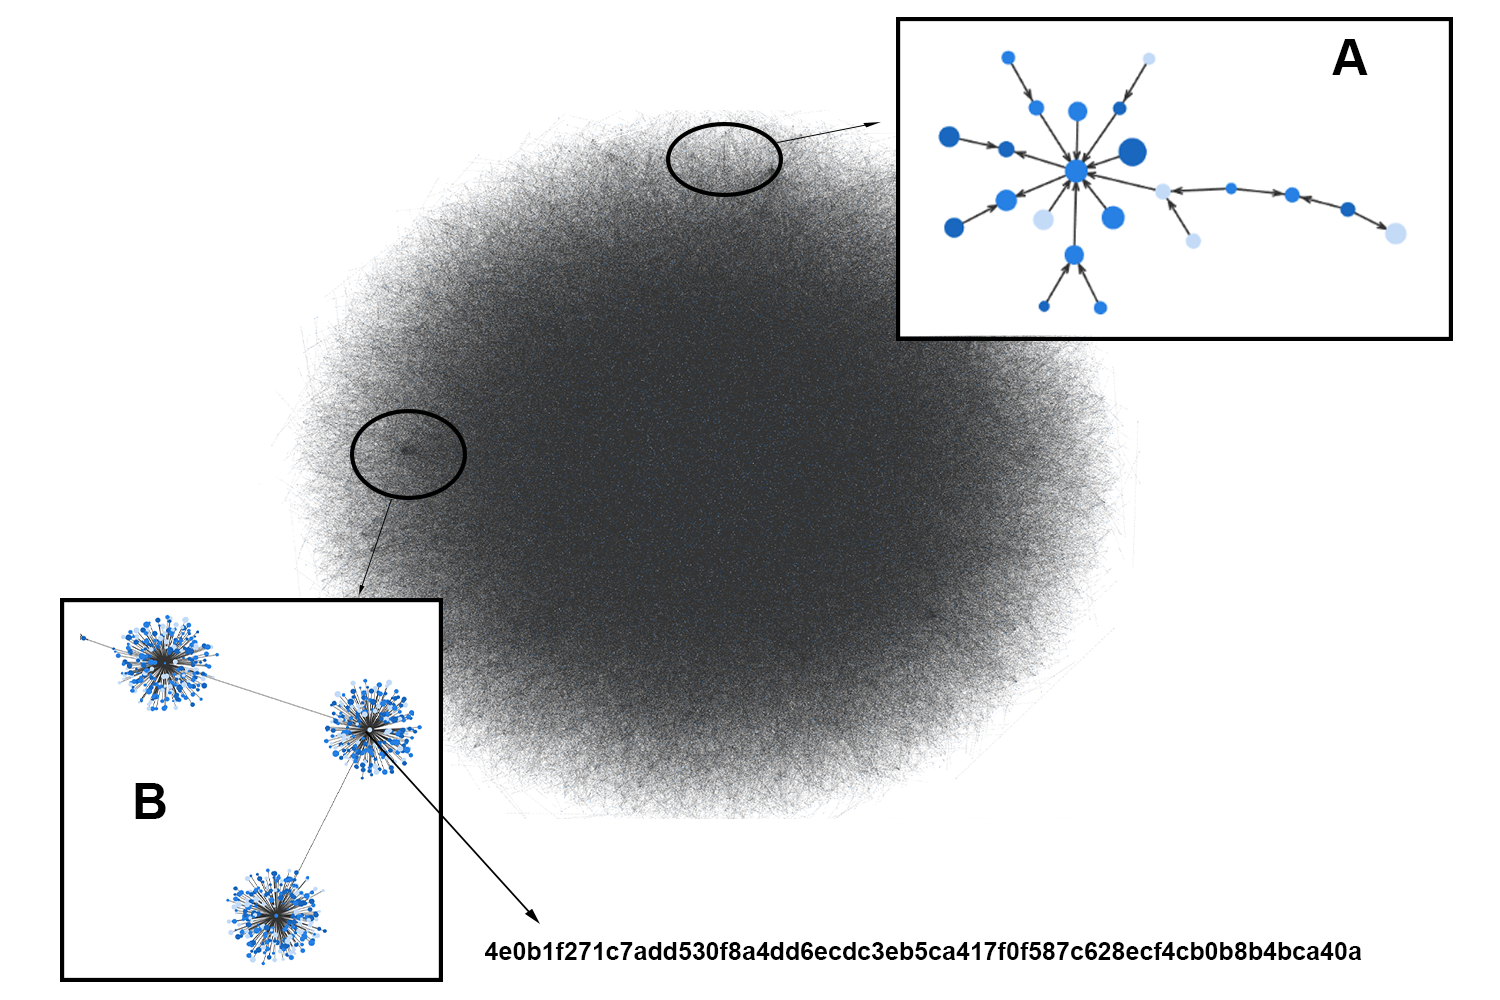
\includegraphics[scale=1.2]{images/demo/graph_tx_demo_presentation.png}
\caption{Porzione di grafo delle transazioni visualizzata attraverso SpyJSBlocks.}
\label{fig:visgraphTx}
\end{figure}

\begin{example}
Consideriamo lo zoom \say{B} della Figura \ref{fig:visgraphTx}. Possiamo notare 3 comunità di nodi, in cui solo uno di esso spedice bitcoin ad un altra comunità.\\
  Prendendo in considerazione il nodo con  identificativo di transazione \say{4e0b1f\-271c7add\-530f8a4dd6e\-cdc3eb5ca41\-7f0f587c6\-28ecf4cb0\-b8b4b\-ca40a}, si può notare attraverso l'uso di uno explorer che la transazione contiene 236 transazioni di input e 1 transazione di output, questo potrebbe indicare che il wallet abbia raggruppato tutte le transazioni su un unico address.
\end{example}

La blockchain di bitcoin serializza i blocchi all'interno di file chiamati \say{blk00000.dat} dove \say{00000} rappresenta l'indice dei file; Bitcoin-core stabilisce degli standard di dimensione per i file, pari a 100 Mb per ogni file.\\
SpyCBlock effettua la serializazione 1 a 1, cioè per ogni file \say{blk0000.dat} produce un file con le informazioni in un specifico formato ad esempio \say{blk00000.json}; questo dà la possibilità di far evolvere facilmente il parser verso un' implementazione parallela e/o distribuita.

\section{Grafo degli address} \label{sec:solGraphAddress}

Dopo avere implmentato la  costruzione del grafo delle transazioni, ci siamo concentrati sulla costruzione del grafo degli address. Come descritto nella Sezione \ref{sec:grafoDegliAddressProblema}, la costruzione di tale grafo introduce alcune problematiche che obbligano a rivedere il modo in cui si ricavano i dati durante il parsing delle informazioni.\\
Gli address sono infatti contenuti all'interno dello script di blocco di una transazione, come illustrato nelle Sezioni \ref{sec:bitcoinScriptBitcoin} e \ref{sec:bitcoinScriptBitcoinCore}, mentre lo script di sblocco contiene solo le informazioni riguardanti le condizioni per cui un UTXO può essere sbloccato, non possedendo nessun riferimento dell'indirizzo di origine.
Per accedere allo script di blocco della precedente transazione, il cui identificativo (hash) risiede all'interno della transazione di input, appartenente alla transazione attualmente analizzata, bisogna memorizzare la cronologia delle transazioni decodificate e ricostruire un meccanismo per la gestione degl'UTXO, simile al meccanismo usato da Bitcoin-core: fornire un metodo di memorizzazione, che consente di prelevare una transazione precedentemente analizzata con costo $O(1)$ oppure con un costo logaritmico $O(N log(N))$.\\
Al momento della stesura del documento, il parser non possiede nessun meccanismo di analisi degli script; essi con il passare del tempo sono diventati molto complessi e, come illustrato nella Sezione \ref{sec:noStrandardScript}, sono stati   introdotti metalinguaggi (come miniscript) per facilitare la scrittura di script \say{no standard}. Questo comporta la necessità di studiare in modo approfondito gli script per ottenere da essi maggiori informazioni.

 \begin{example}\label{ex:probleGraphAddress}

Consideriamo l'address \say{3CD1\-QW6fjg\-TwKq3Pj\-97nty28W\-ZAVkz\-iNom}, coinvolto in numerose truffe e illustrato all'interno dell'articolo \cite{DBLP:conf/icdm/OggierPD18}; tale address è originato da uno script (perché esso utilizza la convenzione del numero 3 come prima cifra) e potrebbe a sua volta contenere più address primitivi al suo interno e quindi rappresentare uno script P2MS oppure potrebbe rappresentare un address ricavato da uno script \say{no standard}. Un esempio di \say{script no standard} è illustrato attraverso il Codice \ref{code:complexscript}.\\
   Gli address originati da script, costringono ad un'analisi più approfondita per ottenere maggiori informazioni sulla loro vera identità; come illustrato nella Sezione \ref{sec:p2shBitcoin}, lo script P2SH è stato il primo esempio di script ad introdurre la possibilità di generare un address non primitivo, seguito dagli script P2WSH, P2WPKH e gli script \say{no standard}.\\
   Come possiamo osservare dalla Sezione \ref{sec:p2shBitcoin}, il processo di verifica di uno script P2SH costringe ad inserire all'interno dello script di sblocco anche lo script P2MS conosciuto come script di riscatto; questa informazione comporta l'analisi dello script di sblocco oltre che dallo script di blocco.\\
   Considerando la transazione con identificativo
   $$\say{82\-a69\-be69e\-00937\-91ab7\-d3803\-69ec\-ffba4f\-1fe08\-27a862\-5ede9\-d89e9\-4776b\-c21}$$

   \noindent bloccata attraverso lo script da cui è originato l'address \say{3CD1\-QW6fjg\-TwKq3Pj\-97nty28W\-ZAVkz\-iNom}, possiamo osservare che la transazione viene \say{consumata} da una nuova transazione con il seguente identificativo:
   $$\say{457\-b5bde2\-35dcf08\-de41597\-68c4f7\-abcb96\-97e1\-760a\-13e6\-caa15a\-7a2d8\-c909\-78}$$

   \noindent Quest'ultima all'interno dello script di sblocco contiene le informazioni necessarie per lo sblocco della transazione bloccata dall'address \say{3CD1\-QW6fjg\-TwKq3Pj\-97nty28W\-ZAVkz\-iNom}.\\
   Attraverso il Codice \ref{code:scriptPubKeyScam} possiamo osservare lo script di blocco da cui è originato l'address \say{3CD1\-QW6fjg\-TwKq3Pj\-97nty28W\-ZAVkz\-iNom}, dove possiamo osservare la condizione di sblocco di uno script P2SH in cui il valore \say{735d4de855597997b21588cc78ca2db696be1c5d} rappresenta l'HASH160 dello script P2MS.
   \begin{lstlisting}[language=bitcoinscript, label={code:scriptPubKeyScam}, caption={Script da cui è originato l'address preso in esempio.}]
      OP_HASH160 735d4de855597997b21588cc78ca2db696be1c5d OP_EQUAL
   \end{lstlisting}
   La condizione necessaria per sbloccare la transazione bloccata con lo script precedente è contenuta all'interno della transazione con identificativo
   $$\say{457\-b5bde2\-35dcf08\-de41597\-68c4f7\-abcb96\-97e1\-760a\-13e6\-caa15a\-7a2d8\-c909\-78}$$
   \noindent Il Codice \ref{code:scritpSigScam} riporta l'intero script di sblocco.

     \begin{lstlisting}[language=bitcoinscript, label={code:scritpSigScam}, caption={Script con cui è possibile eseguire con successo lo script illustrato attraverso il Codice \ref{code:scriptPubKeyScam}.}]
      OP_0 304402203638fc4c33f325d1c62c8feb4979d91300723f4766686e89de7380b269eec
        c7602206d65886d69ccedc33de8f2840f27295b53dd9f9fd637b970664385b47c128da901
        3045022100e8910b2162c08ec560d5737d09d361c07f90bfe58ee4e66a4fbebe246ea2b32c
        02207fb1fc6296213b11ecb2eef3a375c8509776f75880ad5372417b55215fcdf74f01
      OP_PUSHDATA1 522103385adff37fd3d0a620ebc4e9866e81dda8ba8616e5ebcae899c7f51899267
        ae721034c08511718f947d1a3e152195c5e2756588e3e0c2c7730927eb6647af494210721033d
        a9f8938a5b947a723df21b73fbd3985b719249324d2c705acfb97d63a5df9e53ae
     \end{lstlisting}

     Dal precedente script possiamo estrarre lo script di riscatto contenuto dopo l'operatore OP\_PUSHDATA1; il Codice \ref{code:p2msScam} illustra lo script nel formato decodificato.
     \begin{lstlisting}[language=bitcoinscript, label={code:p2msScam}, caption={Readme Script contenuto all'interno dello script di sblocco \ref{code:scritpSigScam}.}]
      OP_2 03385adff37fd3d0a620ebc4e9866e81dda8ba8616e5ebcae899c7f51899267ae7 034c08511718f947d1a3e152195c5e2756588e3e0c2c7730927eb6647af4942107 033da9f8938a5b947a723df21b73fbd3985b719249324d2c705acfb97d63a5df9e OP_3 OP_CHECKMULTISIG
    \end{lstlisting}
    Dal Codice \ref{code:p2msScam} si possono notare 3 chiavi pubbliche differenti:
    \begin{itemize}
      \item \say{0338\-5adff37\-fd3d0a62\-0ebc4e98\-66e81dd\-a8ba8616\-e5ebcae89\-9c7f518\-9926\-7ae7};
      \item \say{034c\-0851\-1718f947\-d1a3e152\-195c5e2756\-588e3e0c2c\-7730927\-eb6647a\-f494\-2107};
      \item \say{033\-da9f8\-938a5b9\-47a723df\-21b73fbd3\-985b719249\-324d2c70\-5acfb97d\-63a5\-df9e}.
    \end{itemize}
    Le precedenti chiavi pubbliche rappresentano identità differenti appartenenti allo stesso wallet oppure a wallet differenti, utilizzando il codice descritto nell'Appendice \ref{sec:buildAddressFromPubKey}, possiamo ricavare un address primitivo dalle precedenti chiavi pubbliche, ottenendo i seguenti address:
    \begin{itemize}
      \item \say{14r7XjPtqVijLRhY9BkGAtDqVDp4txsK1X};
      \item \say{1GryVw5pfa8a1Sc69PXywGLRDZJWc1C6wT};
      \item \say{1G9VBMkqDzPmYxnFMkNxWGmfuQz1CHSYP6}.
    \end{itemize}

    Questo esempio mostra la necessità di analizzare attentamente gli address non primitivi, con i rispettivi script, perché potrebbero contenere informazioni rilevanti per la costruzione del grafo di address, in quanto quest'ultimo deve poter rappresentare il reale flusso di bitcoin tra gli address.\\
    Riesaminando l'esempio appena descritto, dove l'address \say{3CD1\-QW6fjg\-TwKq3Pj\-97nty28W\-ZAVkz\-iNom} viene catalogato come address di \emph{scam}, dopo aver condotto un'attenta analisi sullo script da cui è originato l'address si può concludere che lo script nasconde 3 chiavi pubbliche al suo interno.\\
    Non effettuando quest'ultima analisi, ogni singolo address potrebbe operare singolarmente all'interno della blockchain di Bitcoin passando inosservato agli algoritmi di analisi.
 \end{example}

 Attraverso l'Esempio \ref{ex:probleGraphAddress}, possiamo notare come sia possibile costruire due tipi di grafi di address utilizzando le informazioni estratte dalla blockchain di Bitcoin:
 \begin{itemize}
   \item Il grafo naturale di address, che utilizza solo le informazioni contenute all'interno delgli script di blocco. A titolo d'esempio, il frammento di grafo descritto dalla transazione illustrata nell'esempio \ref{ex:probleGraphAddress} con  identificativo \say{82\-a69\-be69e\-00937\-91ab7\-d3803\-69ec\-ffba4f\-1fe08\-27a862\-5ede9\-d89e9\-4776b\-c21} viene rappresentato dalla Figura \ref{fig:addGrapjNatural}.
   \begin{figure}[H]
   \centering
   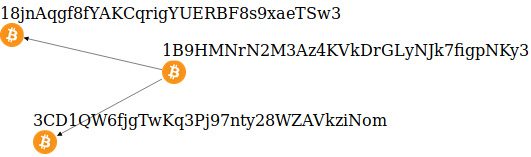
\includegraphics[scale=0.35]{images/exampleWithGraph/naturalAddressGrahScamTx.png}
   \caption{Frammento del grafo naturale degli address descritto dalla transazione con identificativo 82\-a69\-be69e\-00937\-91ab7\-d3803\-69ec\-ffba4f\-1fe08\-27a862\-5ede9\-d89e9\-4776b\-c21.\label{fig:addGrapjNatural}}
   \end{figure}

   Il grafo naturale di address risulta essere troppo superficiale, perché le chiavi pubbliche che fanno parte dello script da cui è ottenuto l'address \say{3CD1\-QW6fjg\-TwKq3Pj\-97nty28W\-ZAVkz\-iNom} potrebbero essere riutilizzate singolarmente all'interno della blockchain di Bitcoin passando inosservate agli algoritmi di analisi;
   \item Il grafo degli address ottenuto con un'analisi degli indirizzi originati da script. A titolo d'esempio, il frammento di grafo illustrato nella Figura \ref{fig:addGrapjNatural} in cui viene condotta un'analisi dello script da cui viene originato l'address \say{3CD1\-QW6fjg\-TwKq3Pj\-97nty28W\-ZAVkz\-iNom} viene illustrato nella Figura \ref{fig:addGraphAnalisis}
   \begin{figure}[H]
   \centering
   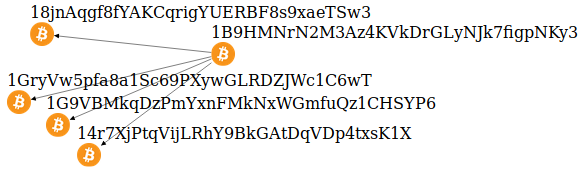
\includegraphics[scale=0.35]{images/exampleWithGraph/decode-address-graph-scam.png}
   \caption{Frammento del grafo degli address ottenuto attraverso un analisi dell'address 3CD1\-QW6fjg\-TwKq3Pj\-97nty28W\-ZAVkz\-iNom.\label{fig:addGraphAnalisis}}
   \end{figure}
   Il grafo di address appena descritto risolve la problematica riguardante le chiavi pubbliche, contenute all'interno dello script, con la conseguenza della perdita del riferimento riguardante l'address originato dallo script, il che aumenta notevolemente il grado di complessità del grafo.\\
   Una possibile soluzione, potrebbe essere quella di utilizzare una rappresentazione attraverso il grafo naturale rappresentato dalla Figura \ref{fig:addGrapjNatural}, con l'aggiunta delle chiavi pubbliche ricavate dallo script come proprietà del nodo, ottenendo la rappresentazione illustrata in Figura \ref{fig:addGrapjNaturalPlus}
   \begin{figure}[H]
   \centering
   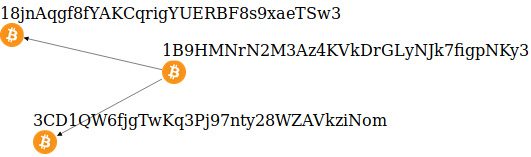
\includegraphics[scale=0.35]{images/exampleWithGraph/naturalAddressGrahScamTx.png}
   \caption{Frammento del grafo naturale degli address arricchito delle informazioni delle chiavi pubbliche all'interno del nodo.\label{fig:addGrapjNaturalPlus}}
   \end{figure}
 \end{itemize}

 In seguito allo studio di fattibilità sulla creazione del grafo, ci siamo limitati alla costruzione di un grafo semplificato, anche perché oltre alle problematiche descritte abbiamo dovuto affrontare anche le problematiche sulla serializzazione delle transazioni M:N (molti a molti): ogni transazione può contenere, infatti, M transazioni di input e N transazioni di output.\\
 Questa caratteristica riguardante il numero di transazioni può essere risolta utilizzando una rappresentazione a multigrafo degli address.
 In questo documento, proponiamo una soluzione in cui si forza l'utilizzo di un comune grafo, in cui ogni transazione M:N viene serializzata in maniera iterativa: la prima transazione di input viene serializzata con tutte le transazioni di output e così a seguire, per le restanti transazioni di input, ignorando per il momento il problema delle chiavi pubbliche contenute all'interno degli script da cui si originano address.
 Un frammento del grafo rappresentante una transazione M:N è illustrato dalla Figura \ref{fig:iterativeAddTx}

\begin{figure}
\centering
 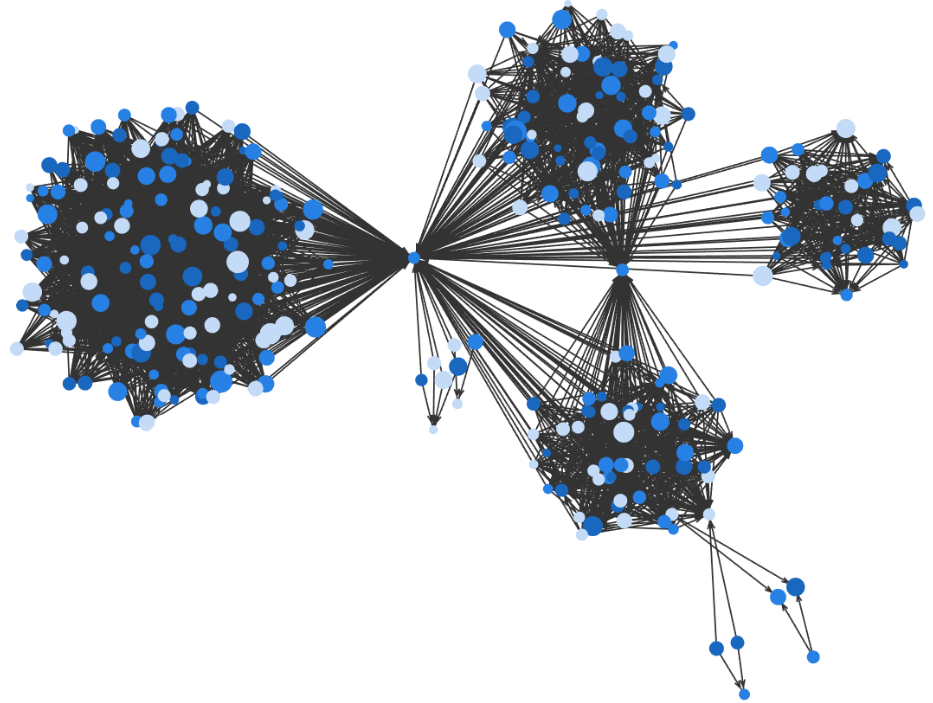
\includegraphics[scale=0.35]{images/demo/iterationTx.png}
 \caption{Frammento del grafo degli address, in cui viene rappresentata una serializzazione iterativa di una transazione M:N.}
 \label{fig:iterativeAddTx}
\end{figure}

 La costruzione del grafo attraverso SpyCBlock avviene grazie all'introduzione del sottomodulo SpyCBlockRPC descritto nella Sezione \ref{sec:spycblockrpc}, il quale si occupa di accedere alle informazioni della transazione precedente tramite l'utilizzo del framework RPC di Bitcoin-core descritto nella Sezione \ref{sec:jsonrpchttp}.
 Il parser inoltre utilizza il framework RPC per decodificare lo script di blocco, da cui si ottiene l'address oppure gli address contenuti al suo interno.\\
 Il framework RPC di Bitcoin-core non essendo adatto all'estrazione completa delle informazioni dalla blockchain di Bitcoin limita le prestazioni del parser durante l'analisi delle informazioni.\\
 Questo problema potrebbe essere risolto estendendo l'implementazione di SpyCBlockRPC ad un implementazione \emph{multi thread} oppure implementando un decompilatore per gli script di Bitcoin; quest'ultima soluzione implica anche l'implementazione di un metodo di memorizzazione per mantenere una cronologia delle transazioni decodificate dal parser.

 Una porzione di grafo degli address viene rappresentata dalla Figura \ref{fig:addressGraph}

\begin{figure}
\centering
 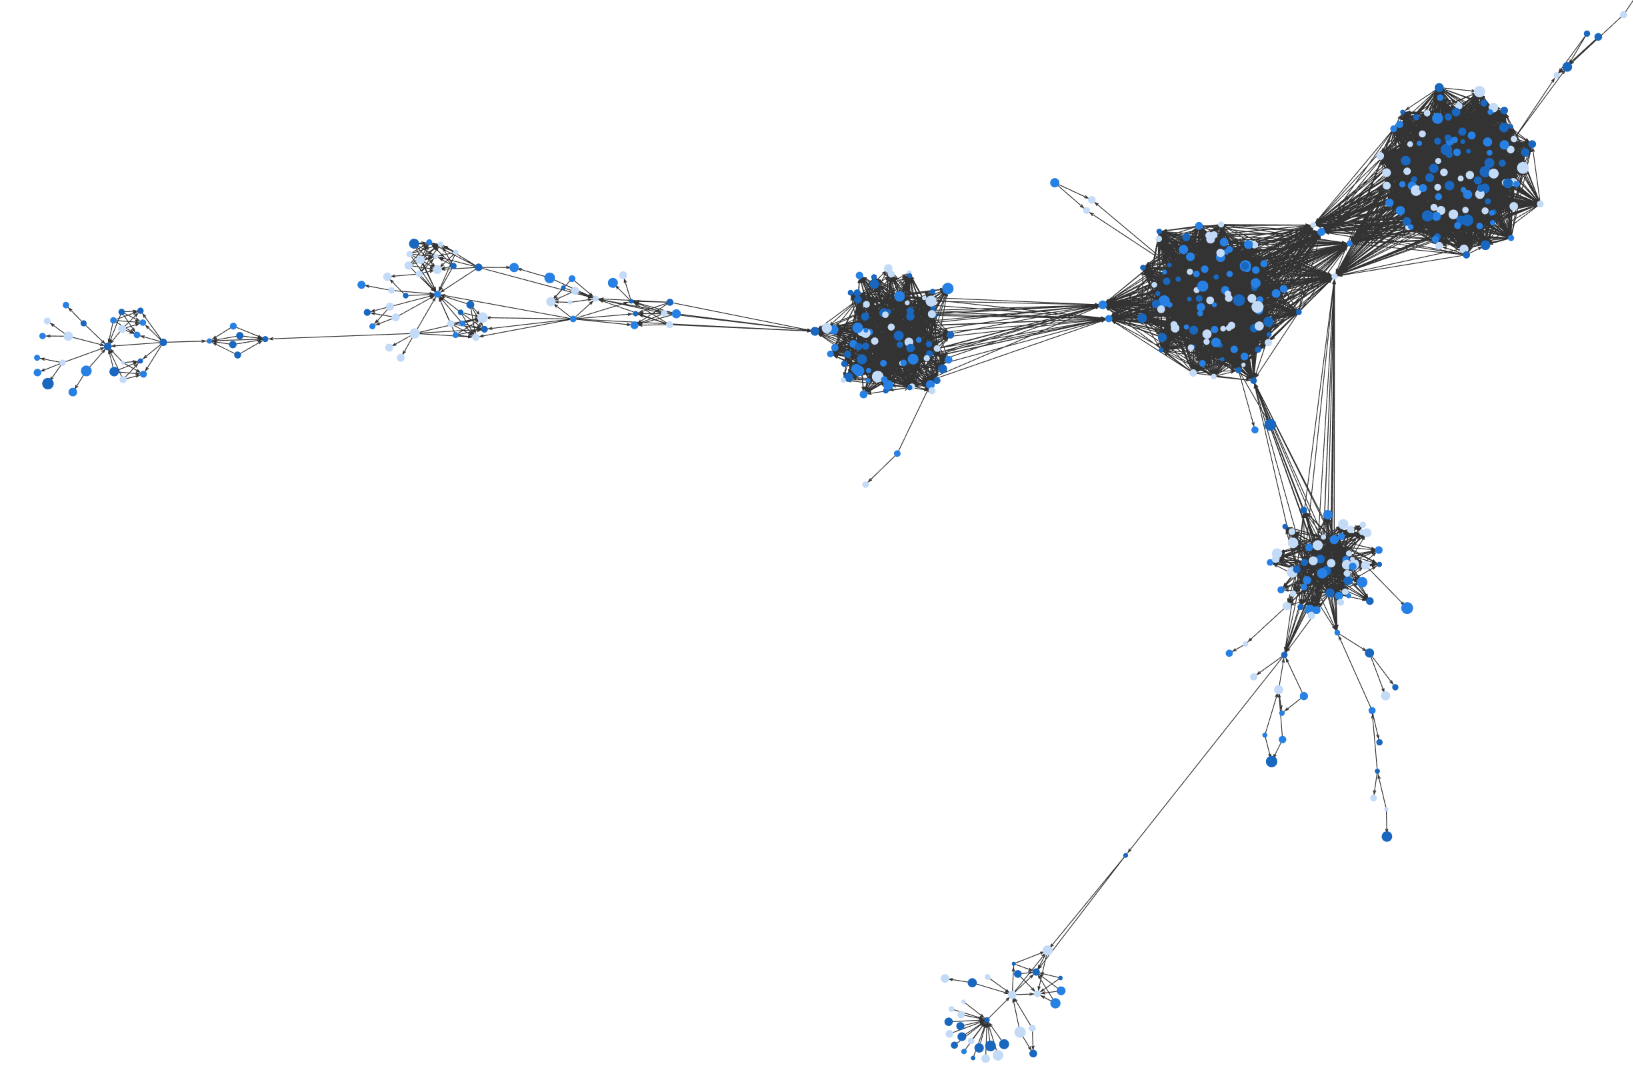
\includegraphics[scale=0.25]{images/demo/address_graph.png}
 \caption{Frammento del grafo degli address estrapolato dalla demo descritta nella Sezione \ref{sec:SpyJSBlocks}.}\label{fig:addressGraph}
\end{figure}

\section{Risultati Sperimentali} \label{sec:valutazionesperimentale}

La soluzione proposta si è limitata all'estrazione dei dai dalla blockchain di Bitcoin in maniera scalabile con una successiva riconversione dei dati tale da consentire la costruzione di un grafo di transazioni, oltre alla serializzazione completa in JSON della blockchain.\\
Il parser proposto come soluzione oltre a serializzare il grafo di transazioni implementa anche una soluzione sperimentale per la creazione del grafo di address attraverso l'ausilio del framework RPC di Bitcoin descritto nella Sezione \ref{}.\\
La valutazione sperimentale condotta si limita ad analizzare le tempistiche di analisi solo per la serializzazione in JSON della blockchain e per la serializzazione del grafo di transazioni, ignorando le tempistiche di serializzazione del grafo di address perchè risultano essere molto elevate a causa della dipendenza diretta con il framework RPC.\\
L'analisi viene condotta eseguendo il parser su un laptop con una CPU DESCRIVI LA CPU, 


\section{DEMO} \label{sec:solDemo}

\subsection{AnalyticsPyBlock} \label{sec:AnalyticsPyBlock}

Per dimostrare un possibile utilizzo della blockchain di Bitcoin serializzata in JSON è stata sviluppato un semplice strumento di analisi denominato AnalyticsPyBlock, il quale permette anche di sviluppare analisi personalizzate.\\
AnalyticsPyBlock al momento della stesura del documento supporta solo un tipo di analisi, riguardante la tipologia di script utilizzati nel tempo nella rete Bitcoin; il software di analisi viene sviluppato in Python3 e risiede su Github sotto licenza Apache License 2.0.\\
La Figura \ref{fig:analisisScript} illustra il risultato dell'analisi sulle tipologie di script.

\begin{figure*}
	\centering
	\subfigure[][Grafico che rappresenta gli script più utilizzati all'interno la blockchain di Bitcoin.]{\label{fig:globalAnalisis}
		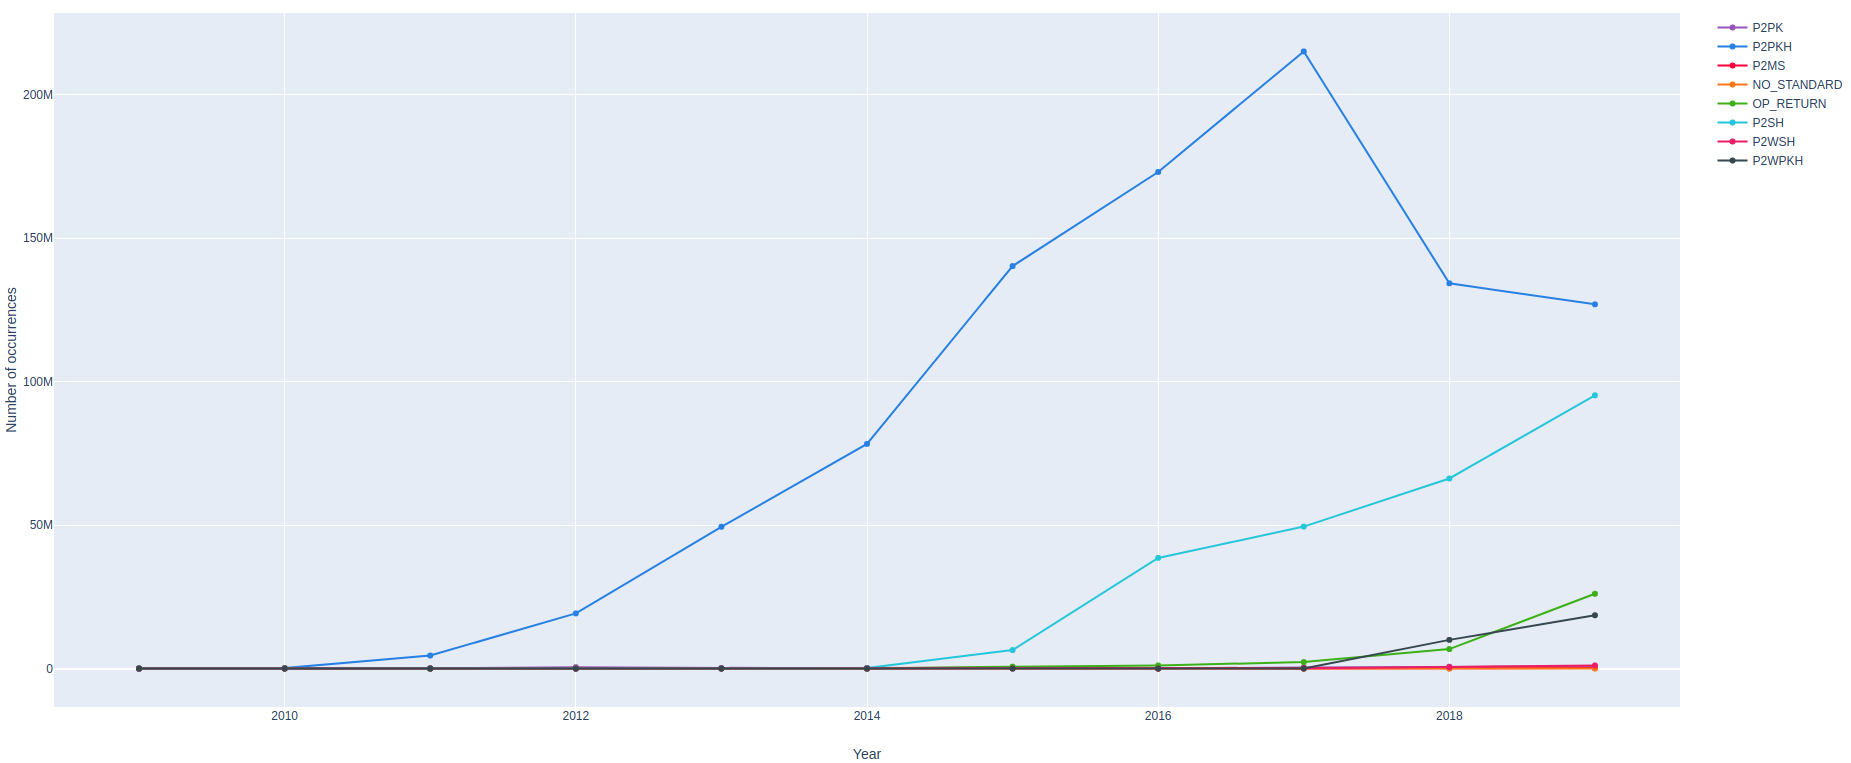
\includegraphics[width=.8\linewidth]{images/demo/analytics/result-global.png}}
	\subfigure[][Grafico che rappresenta l'utilizzo dello script OP\_RETURN per archiviare dati.]{\label{fig:optReturnScript}
		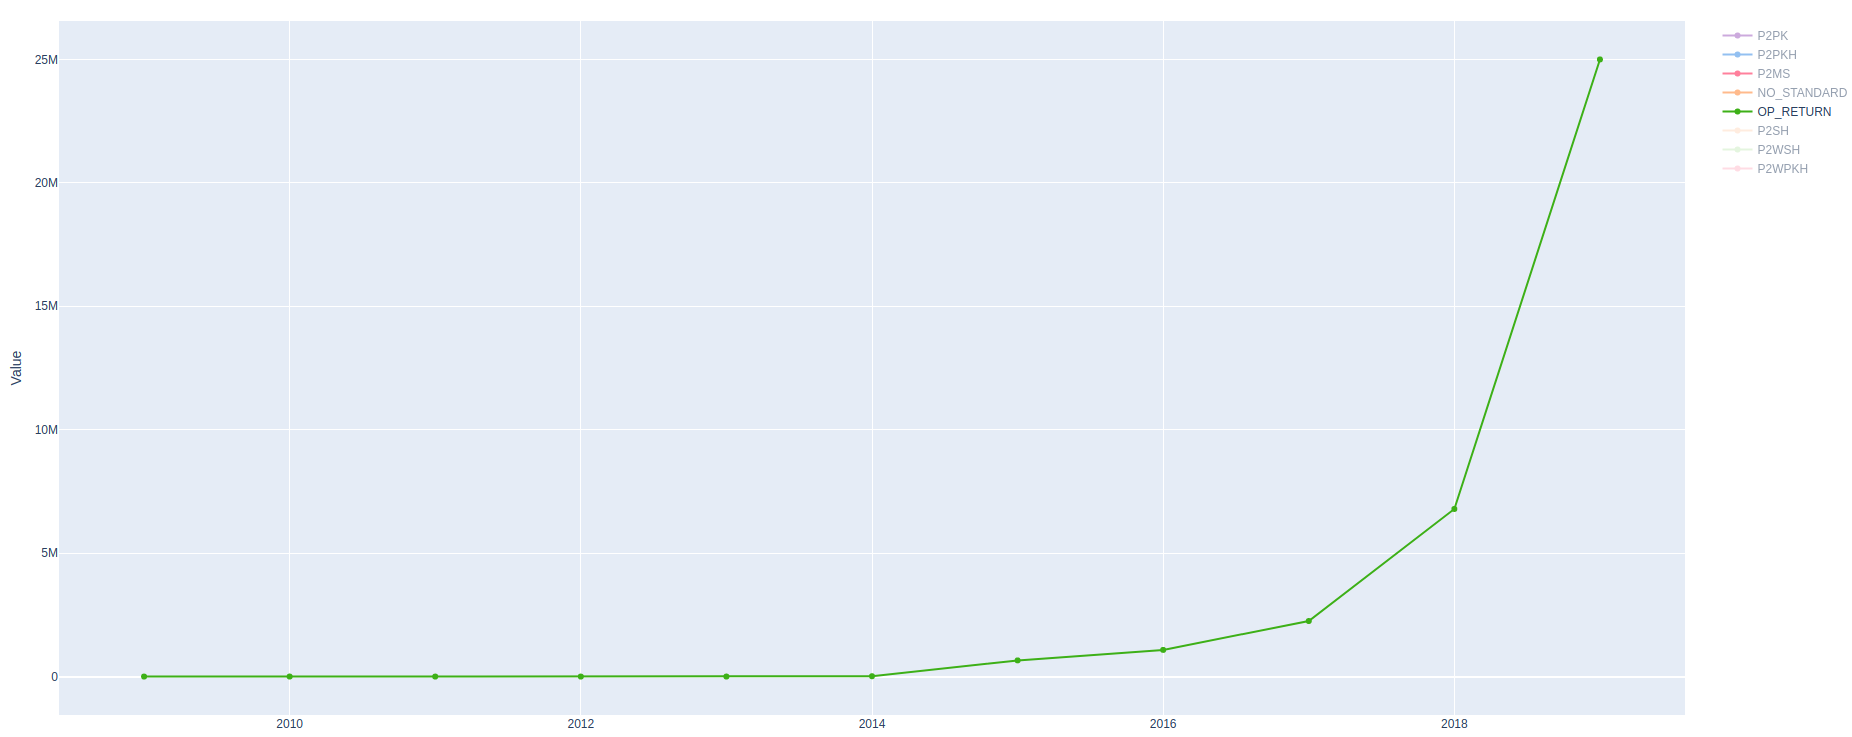
\includegraphics[width=.8\linewidth]{images/demo/analytics/opt_return.png}}
	\caption{Grafici estrapolati dalla demo descritta nel segunte capitolo.}
	\label{fig:analisisScript}
\end{figure*}

%    \begin{figure}
%    \begin{subfigure}{\textwidth}
%      \centering
%      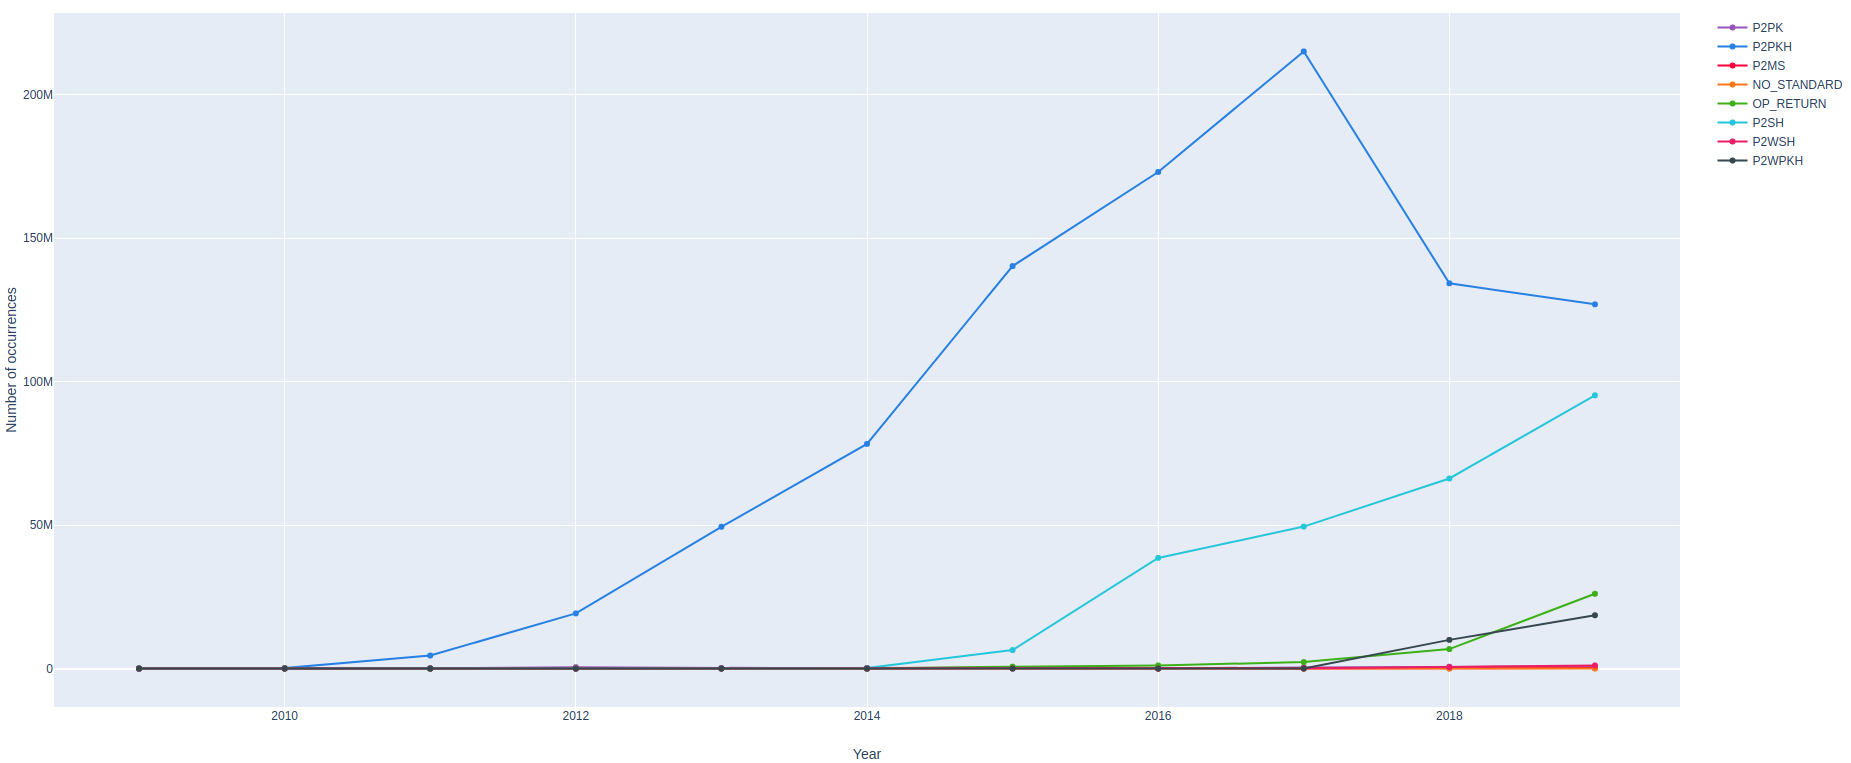
\includegraphics[width=.8\linewidth]{images/demo/analytics/result-global.png}
%      \caption{1a. Grafico che rappresenta gli script più utilizzati all'interno la blockchain di Bitcoin.}
%      \label{fig:globalAnalisis}
%    \end{subfigure}%
%    \begin{subfigure}{\textwidth}
%      \centering
%      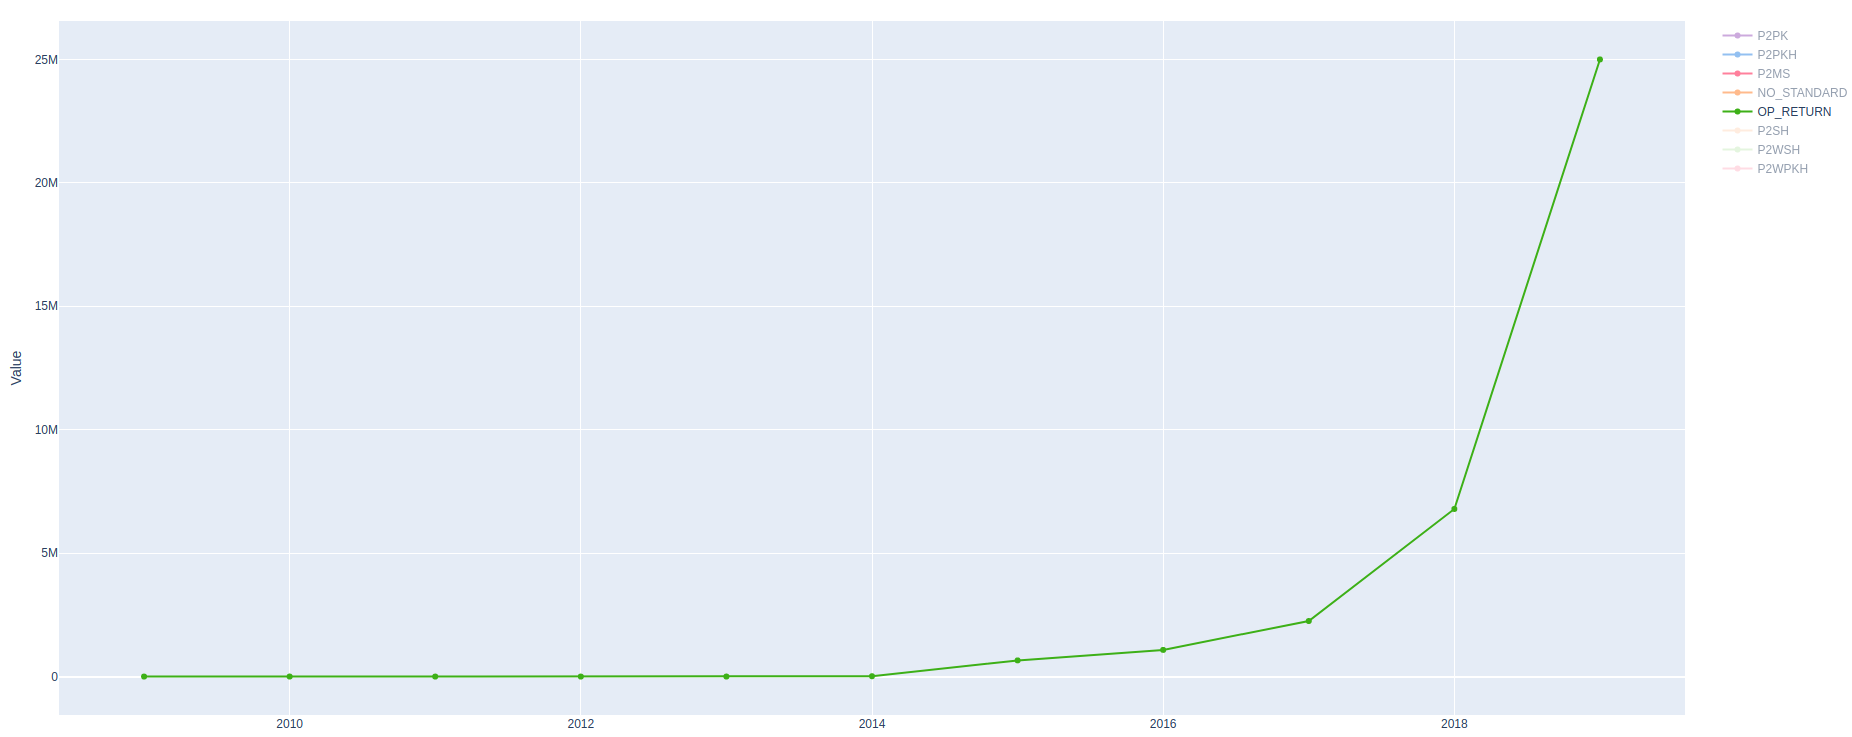
\includegraphics[width=.8\linewidth]{images/demo/analytics/opt_return.png}
%      \caption{1b.  Grafico che rappresenta l'utilizzo dello script OP\_RETURN per archiviare dati.}
%      \label{fig:optReturnScript}
%    \end{subfigure}
%    \caption{Grafici estrapolati dalla demo descritta nel segunte capitolo.}
%    \label{fig:analisisScript}
%    \end{figure}

La Figura \ref{fig:globalAnalisis} mostra gli script maggiormente utilizzati, che risultano essere P2PKH e  P2SH; inoltre la Figura \ref{fig:optReturnScript} mostra l'utilizzo della blockchain di Bitcoin per l'archiviazione di dati. Questa informazione è molto utile ai fini della costruzione del grafo perchè attraverso una futura operazione di \emph{data cleaning} si possono eliminare tutte le informazioni che riguardano l'archiviazione di dati attraverso l'operatore OP\_RETURN.\\
La strumento impiega meno di 12 ore per analizzare i file JSON serializzati da SpyCBlock; anche tale tool potrebbe essere migrato ad un'implementazione multiprocessore con cui si può migliorare la velocità di analisi.

\subsection{SpyJSBlocks} \label{sec:SpyJSBlocks}

Per visualizzare i grafi serializzati da SpyCBlock abbiamo sviluppato un applicazione web che fa uso delle librerie appartenenti alla famiglia ngraph descritte nella Sezione \ref{sec:ngraph}, con cui siamo riusciti ad ottenere una visualizzazione di una piccola parte dei grafi serializzati da SpyCBlock.\\
Attraverso la possibilità di visualizzare i grafi, siamo riusciti ad eseguire tutte le analisi discusse in questo documento; inoltre con l'utilizzo del modulo ngraph.louvian abbiamo condotto un'analisi minimale sul grafo degli address scomponendo quest'ultimo in comunità, anche se l'applicazione di tale algoritmo soffre delle problematiche descritte nella Sezione \ref{sec:solGraphAddress}.\\
L'applicativo web viene sviluppata utilizzando JavaScript senza l'ausilio di framework; una possibile evoluzione di questo applicativo potrebbe essere la migrazione ad un framework come React \cite{vis:react}.\\
Lo strumento software possiede due diverse implementazioni per via delle diverse problematiche riguardanti le librerie ngraph descritte nella Sezione \ref{sec:ngraph}; l'applicativo risiedono su Github sotto licenza Creative Commons 4.0 e vengono deniminati SpyJSBlock \cite{vis:SpyJSBlock} e SpyJSBlock-NGraph \cite{vis:SpyJSBlock-Ngraph}.
Le principali differenze tra gli strumenti software sono:
\begin{itemize}
  \item SpyJSBlock è una prima implementazione dell'applicativo web che fa uso della libreria VivagraphJS descritta nella sezione \ref{sec:ngraph}, per via della difficoltà nel personalizzare il rendering tramite WebGl non viene eseguita nessuna personalizzazione eccetto l'aggiunta della possibilità di esplorare il nodo del grafo attraverso eventi di click che offrono la possibilità di ricercare l'id della transazione oppure l'address attraverso un'explorer come Explora \cite{blockstream:esplora}.\\
  Non utilizzando nessuna particolare personalizzazione il rendering risulta essere molto veloce, riuscendo a visualizzare una porzione di grafo molto più grande, ma risulta essere difficoltoso cambiare la modalità di rendering oppure applicare algoritmi di analisi sul grafo.\\
  Un frammento di grafo visualizzato attraverso SpyJSBlock viene illustrato attraverso la Figure \ref{fig:vivagraphSpyJSBlock}.

  \begin{figure}
  \centering
   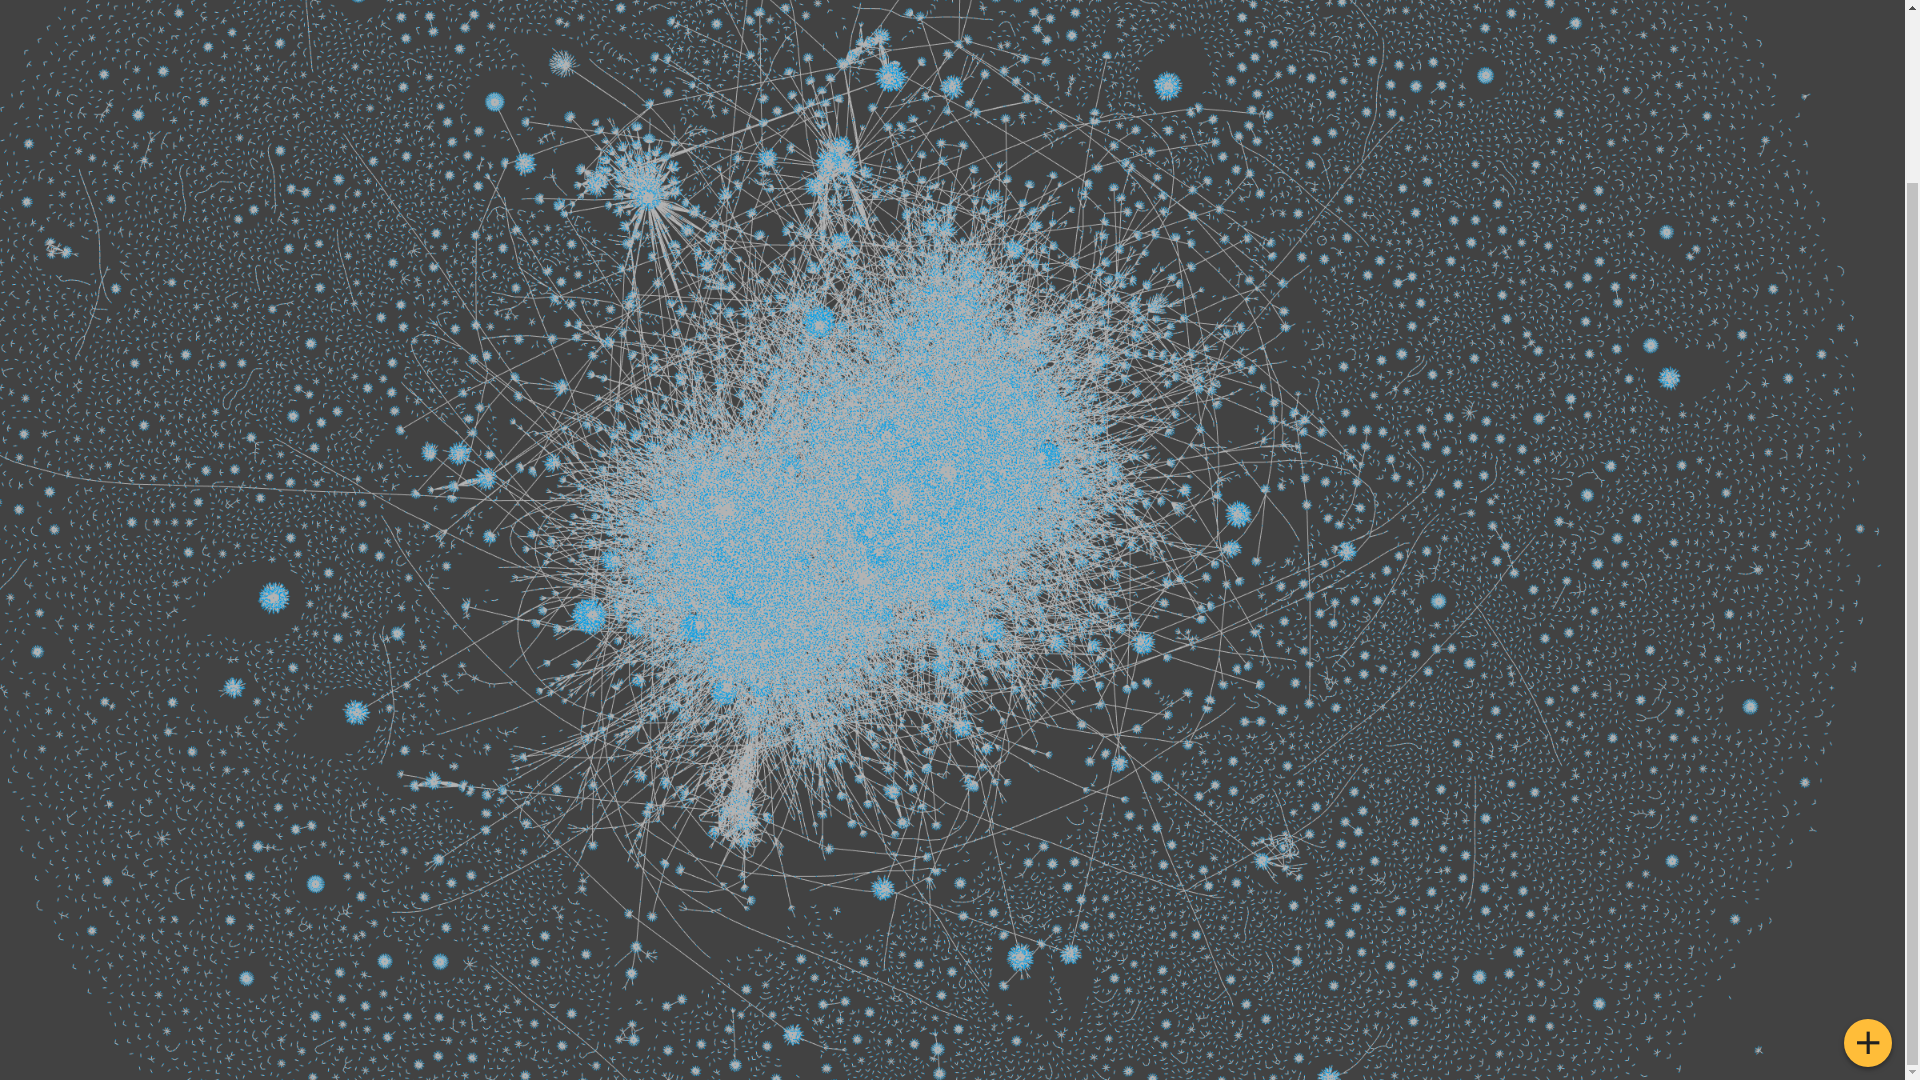
\includegraphics[scale=0.2]{images/demo/vivagraph.png}
   \caption{Frammento del grafo visualizzato attraverso l'applicativo SpyJSBlock.}\label{fig:vivagraphSpyJSBlock}
  \end{figure}

  Per personalizzare il rendering ed avere più controllo sulla visualizzazione del grafo abbiamo sviluppato un'alternativa utilizzando le librerie della famiglia ngraph.
  \item SpyJSBlock-NGraph è un raffinamento dello strumento SpyJSBlock, dove vengono utilizzati i moduli della famiglia ngraph per il rendering dei grafi, con cui si riesce ad ottenere un miglioramento nella qualità del rendering a discapido però delle performance: avendo la possibilità di renderizzare una porzione più piccola del grafo.
  Viene utilizzato il modulo ngraph.pixel per il rendering in 3D del grafo delle transazioni, in cui viene implementata anche la possibilità di ricercare l'id della transazione attraverso l'explorer Explora, La Figura \ref{} illustra un frammento del grafo delle transazioni.
  Per il rendering del grafo degli address invece viene utilizzato il modulo ngraph.pixi con cui si riesce ad ottenere una visualizzazione 2D di un grafo diretto, La Figura \ref{fig:pixiaddress} ne illustra un esempio.
  Inoltre sulla tipologia del grafo di address viene applicato un algoritmo di ricerca delle comunità attraverso il modulo ngraph.louvain descritto nella Sezione \ref{sec:ngraph}.\\
  Dopo l'applazione dell algoritmo, le comunità di nodi vengono dipinde con colori diversi, semplificando l'individuazione di quest'utlime all'interno del grafo.\
  La Figura \ref{fig:pixilouvianaddress} illustra una composizione in comunità del grafo di address.

  \begin{figure}
  \centering
   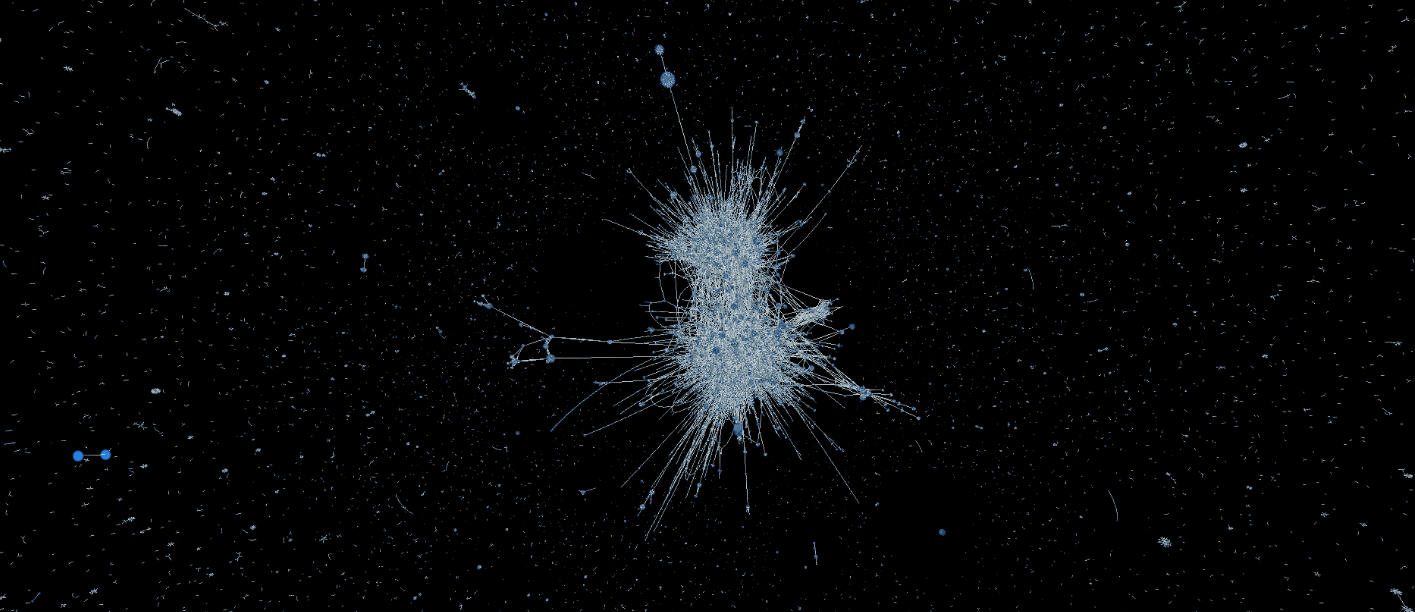
\includegraphics[scale=0.25]{images/demo/3D_tx.png}
   \caption{Frammento del grafo visualizzato attraverso l'applicativo SpyJSBlock.}\label{fig:vivagraphSpyJSBlock}
  \end{figure}

  \begin{figure*}
  	\centering
  	\subfigure[][Grafo di address visualizzato attraverso il modulo ngraph.pixi\cite{vis:ngraph.pixi}.]{\label{fig:pixiaddress}
  		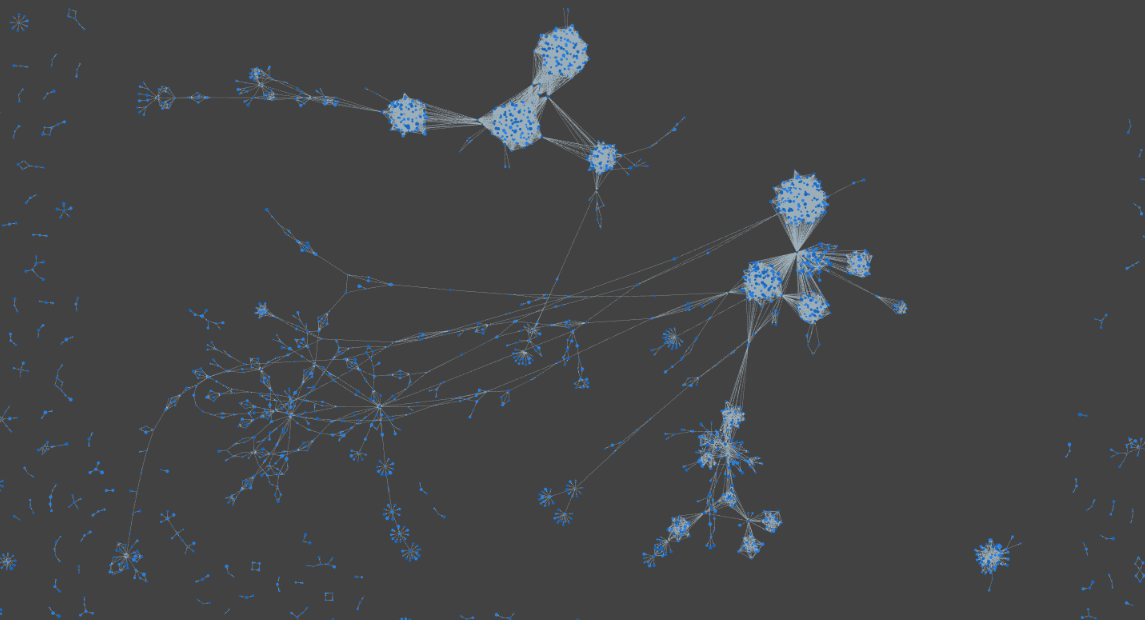
\includegraphics[width=.8\linewidth]{images/demo/ngraphpixi.png}}
  	\subfigure[][Grafo di address scomposto in comunità attraverso l'utilizzo del modulo ngraph.louvian\cite{ngraph.louvain}]{\label{fig:pixilouvianaddress}
  		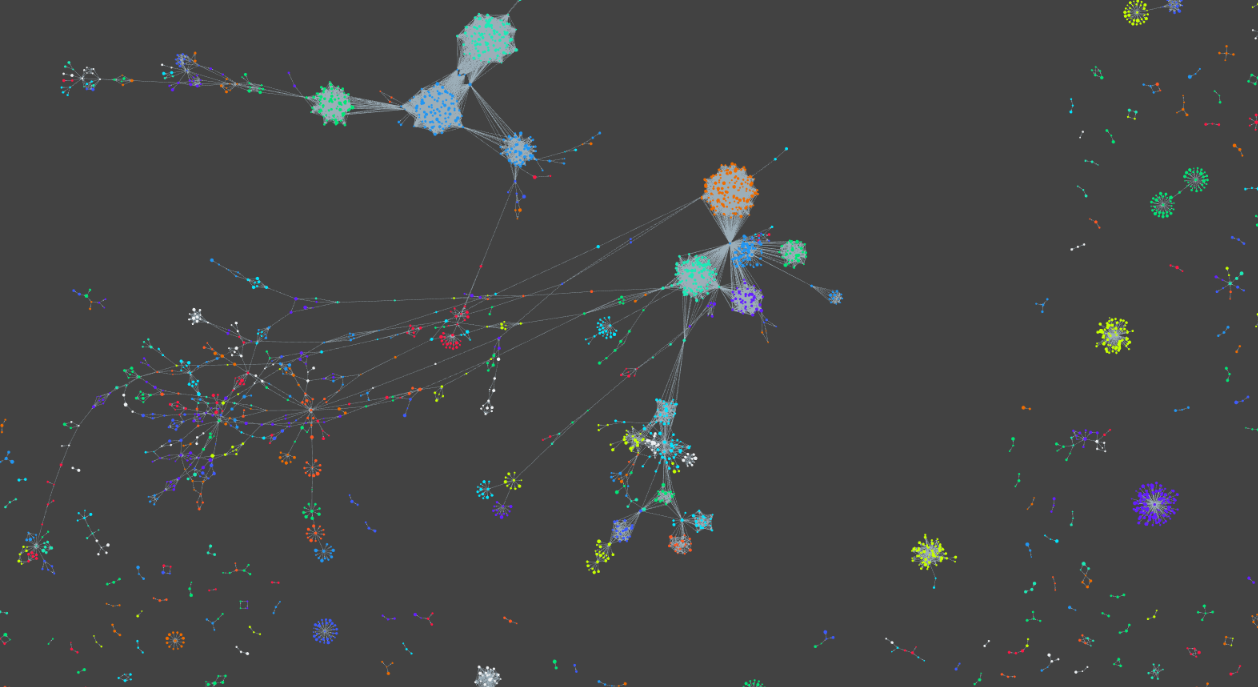
\includegraphics[width=.8\linewidth]{images/demo/ngraphlouvian.png}}
  	\caption{Frammenti di visualizzazione dei grafi estrapolati dalla demo descritta nel segunte capitolo.}
  	\label{fig:ngraphvis}
  \end{figure*}

\end{itemize}

\chapter{Conclusioni}\label{chap:conclusioni}

Il lavoro condotto in questa tesi ha evidenziato  la possibilità di analizzare la blockchain di Bitcoin in modo scalabile. Inoltre, questo studio ha approfondito l'analisi del linguaggio Bitcoin Script e il modo in cui una transazione Bitcoin può essere spesa, facendo emergere la necessità di approfondire ultreiormente l'indagine in questo ambito, poiché le informazioni contenute all'interno degli script possono aggiungere informazioni interessanti per la costruzione del grafo degli address.

I risultati ottenuti attraverso lo sviluppo del parser sono andati ben oltre le nostre aspettative, perché, dopo l'analisi dei numerosi esempi presi in considerazione, come BlockSci, non pensavamo di riuscire a ricavare un prototipo di un software scalabile che potesse venire eseguito su macchine comuni con tempi di calcolo ragionevoli.

Guardando alle possibili estensioni del lavoro svolto, si può pensare di modificare l'implementazione del parser in modo tale da sfruttare il parallelismo, il che  migliorerebbe notevolmente le prestazioni di deserializzazione.\\
Inoltre, attraverso l'utilizzo del prototipo SpyCBlock sono emerse una serie di problematiche riguardante la costruzione del grafo degli address, per via della complessità riguardante gli script di sblocco e blocco di una transazione.

La complessità degli script lascia spazio ad una possibile implementazione di un sottomodulo per l'analisi approfondita di essi, con la necessità però di progettare un metodo per la memorizzazione delle transazioni analizzate. Con l'apporto di queste due modifiche si potrebbe lavorare solo con i file serializzati dal nodo Bitcoin-core senza l'utilizzo del framework RPC, aumentanto così la velocità di analisi per la costruzione del grafo di address.\\
La serializzazione JSON dell'intera blockchain effettuata da SpyCBlock introduce infine la  possibilità di analizzare, attraverso strumenti di analisi di Big Data, la struttura della blockchain di Bitcoin.

%%%%%%%%%%%%%%%%%%%%%%%%%%%%%%%%%%%%%%%%%%%%%%%%%%%%%%%%%%%%%%%

% RINGRAZIAMENTI - PERSONALIZZARE
\ringraziamenti
Grazie a Grazia, Graziella e la sorella.

\appendix
% INCLUSIONE APPENDICI - - PERSONALIZZARE - TENERE COERENTE CON LISTA IN ALTO
\chapter{Appendice}
\label{app:a}


%%%%%%%%%%%%%%%%%%%%%%%%%%%%%%%%%%%%%%%%%%%%%%%%%%%%%%%%%%%%%%%

% INDICI - ELIMINARE GLI INDICI NON NECESSARI

% INDICE DELLE FIGURE
\listoffigures

% INDICE DELLE TABELLE
\listoftables

% INDICE DEI CODICI
\listofcodes

%%%%%%%%%%%%%%%%%%%%%%%%%%%%%%%%%%%%%%%%%%%%%%%%%%%%%%%%%%%%%%%

% BIBLIOGRAFIA
\phantomsection
\addcontentsline{toc}{chapter}{\refname}
\nocite{*}
\printbibliography

\end{document}
